\documentclass[12pt,twoside]{article}

\textwidth 17cm \textheight 25cm \evensidemargin 0cm
\oddsidemargin 0cm \topmargin -2.5cm
\parindent 0pt
%\parskip \bigskipamount

\usepackage{graphicx}
\usepackage[dutch]{babel}
\usepackage{amssymb,amsthm,amsmath}
\usepackage[utf8]{inputenc}
\usepackage{nopageno}
\usepackage{pdfpages}
\usepackage{enumerate}
\usepackage{caption}
\usepackage{wrapfig}
\usepackage{pgf,tikz}
\usepackage{color}
\usetikzlibrary{arrows}
\usetikzlibrary{patterns}
\usepackage{fancyhdr}
\pagestyle{fancy}
\usepackage[version=3]{mhchem}
\usepackage{multicol}
\usepackage{fix-cm}
\usepackage{setspace}
\usepackage{mhchem}
\usepackage{xhfill}
\usepackage{parskip}
\usepackage{cancel}
\usepackage{mdframed}
\usepackage{url}

\newcommand{\todo}[1]{{\color{red} TODO: #1}}

\newcommand{\degree}{\ensuremath{^\circ}}
\newcommand\rad{\qopname\relax o{\mathrm{rad}}}

\newcommand\ggd{\qopname\relax o{\mathrm{ggd}}}

\def\LRA{\Leftrightarrow}%\mkern40mu}

\newcommand{\zrmbox}{\framebox{\phantom{EXE}}\phantom{X}}
\newcommand{\zrm}[1]{\framebox{#1}}

% environment oefening:
% houdt een teller bij die de oefeningen nummert, probeert ook de oefening op één pagina te houden
\newcounter{noefening}
\setcounter{noefening}{0}
\newenvironment{oefening}
{
  \stepcounter{noefening}
  \pagebreak[0]
  \begin{minipage}{\textwidth}
  \vspace*{0.7cm}{\large\bf Oefening \arabic{noefening}}
}{%
  \end{minipage}
}

\usepackage{calc}

% vraag
\reversemarginpar
\newcounter{punten}
\setcounter{punten}{0}
\newcounter{nvraag}
\setcounter{nvraag}{1}
\newlength{\puntwidth}
\newlength{\boxwidth}
\newcommand{\vraag}[1]{
\settowidth{\puntwidth}{\Large{#1}}
\setlength{\boxwidth}{1.5cm}
\addtolength{\boxwidth}{-\puntwidth}
{\large\bf Vraag \arabic{nvraag} \addtocounter{nvraag}{1}}\vspace*{-0.5cm}
{\marginpar{\color{lightgray}\fbox{\parbox{1.5cm}{\vspace*{1cm}\hspace*{\boxwidth}{\Large{#1}}}}}
\vspace*{0.5cm}}
\addtocounter{punten}{#1}}

% arulefill
\newcommand\arulefill[1][]{
  \ifstrempty{#1}{
    \leavevmode{
      \xrfill[-5pt]{0.3pt}[lightgray]
      \endgraf
    }
    \vspace*{0.2cm}
  }{
    \leavevmode{
      \xrfill[-5pt]{0.3pt}[lightgray]
      \endgraf
      \vspace*{0.2cm}
    }
    \foreach \n in {1,...,#1}{
      \leavevmode{
        \xrfill[-5pt]{0.3pt}[lightgray]
        \endgraf
        \vspace*{0.2cm}
      }
    }
  }
}
% \arules{n}
\newcommand{\arules}[1]{
\mbox{}
\color{lightgray}
%\vspace*{0.05cm}
\foreach \n in {1,...,#1}{
  \vspace*{0.75cm}
  \hrule height 0.3pt\hfill
}\color{black}\vspace*{0.2cm}}

% \arule{x}
\newcommand{\arule}[1]{
\color{lightgray}{\raisebox{-0.1cm}{\rule[-0.05cm]{#1}{0.3pt}}}\color{black}
}

% \abox{y}
\newcommand{\abox}[1]{
\fbox{
\begin{minipage}{\textwidth- 4\fboxsep}
\hspace*{\textwidth}\vspace{#1}
\end{minipage}
}
}

\newcommand{\ruitjes}[1]{
\definecolor{cqcqcq}{rgb}{0.85,0.85,0.85}
\hspace*{-2.5cm}
\begin{tikzpicture}[scale=1.04,line cap=round,line join=round,>=triangle 45,x=1.0cm,y=1.0cm]
\draw [color=cqcqcq, xstep=0.5cm, ystep=0.5cm] (0,-#1) grid (20.5,0);
\end{tikzpicture}
}


\newcommand{\assenstelsel}[5][1]{
\definecolor{cqcqcq}{rgb}{0.65,0.65,0.65}
\begin{tikzpicture}[scale=#1,line cap=round,line join=round,>=triangle 45,x=1.0cm,y=1.0cm]
\draw [color=cqcqcq,dash pattern=on 1pt off 1pt, xstep=1.0cm,ystep=1.0cm] (#2,#4) grid (#3,#5);
\draw[->,color=black] (#2,0) -- (#3,0);
\draw[shift={(1,0)},color=black] (0pt,2pt) -- (0pt,-2pt) node[below] {\footnotesize $1$};
\draw[color=black] (#3.25,0.07) node [anchor=south west] { x};
\draw[->,color=black] (0,#4) -- (0,#5);
\draw[shift={(0,1)},color=black] (2pt,0pt) -- (-2pt,0pt) node[left] {\footnotesize $1$};
\draw[color=black] (0.09,#5.25) node [anchor=west] { y};
\draw[color=black] (0pt,-10pt) node[right] {\footnotesize $0$};
\end{tikzpicture}
}

\newcommand{\getallenas}[3][1]{
\definecolor{cqcqcq}{rgb}{0.65,0.65,0.65}
\begin{tikzpicture}[scale=#1,line cap=round,line join=round,>=triangle 45,x=1.0cm,y=1.0cm]
\draw [color=cqcqcq,dash pattern=on 1pt off 1pt, xstep=1.0cm,ystep=1.0cm] (#2,-0.2) grid (#3,0.2);
\draw[->,color=black] (#2.25,0) -- (#3.5,0);
\draw[shift={(0,0)},color=black] (0pt,2pt) -- (0pt,-2pt) node[below] {\footnotesize $0$};
\draw[shift={(1,0)},color=black] (0pt,2pt) -- (0pt,-2pt) node[below] {\footnotesize $1$};
\draw[color=black] (#3.25,0.07) node [anchor=south west] {$\mathbb{R}$};
\end{tikzpicture}
}

\newcommand{\visgraad}[1]{\begin{tabular}{p{0.5cm}|p{#1}}&\\\hline\\\end{tabular}}

\newcommand{\tekenschema}[2]{\begin{tabular}{p{0.5cm}|p{#1}}&\\\hline\\[#2]\end{tabular}}

% schema van Horner
\newcommand{\schemahorner}{
\begin{tabular}{p{0.5cm}|p{7cm}}
&\\[1.5cm]
\hline\\
\end{tabular}}

% geef tabular iets meer ruimte
\setlength{\tabcolsep}{14pt}
\renewcommand{\arraystretch}{1.5}

\newcommand{\toets}[3]{
\thispagestyle{plain}
\vspace*{-2.5cm}
\begin{tikzpicture}[remember picture, overlay]
    \node [shift={(15.25 cm,-1.6cm)}] {%
        \includegraphics[width=1.8cm]{/home/ppareit/kaa1415/logokaavelgem.png}%
    };%
\end{tikzpicture}

\begin{tabular}{|llc|c|}
\hline
\vspace*{-0.5cm}
&&&\\
Naam & \arule{4cm} & {\Large\bf KA AVELGEM} & \\
\vspace*{-0.75cm}
&&&\\
Klas & \arule{4cm} & {\Large\bf 20...-...-...} & \\
\hline
\vspace*{-0.75cm}
&&&\\
Toets & {\bf #2} & {\large\bf #1} & Beoordeling\\
\vspace*{-0.75cm}
&&&\\
Onderwerp & \multicolumn{2}{l|}{\bf #3} &\\
\hline
\end{tabular}
}

\newcommand{\oefeningen}[1]{

\fancyhead[LE, RO]{\vspace{0.5cm} #1}
%\thispagestyle{plain}

{\bf \Large \centering Oefeningen: #1}

}

\raggedbottom

\newcommand\dom{\qopname\relax o{\mathrm{dom}}}
\newcommand\ber{\qopname\relax o{\mathrm{ber}}}

\newcommand\mC{\qopname\relax o{\mathrm{mC}}}
\newcommand\uC{\qopname\relax o{\mathrm{{\mu}C}}}
\newcommand\C{\qopname\relax o{\mathrm{C}}}

\newcommand\W{\qopname\relax o{\mathrm{W}}}
\newcommand\kW{\qopname\relax o{\mathrm{kW}}}
\newcommand\kWh{\qopname\relax o{\mathrm{kWh}}}


\newcommand\V{\qopname\relax o{\mathrm{V}}}
\newcommand\ohm{\qopname\relax o{\mathrm{\Omega}}}
\newcommand\kohm{\qopname\relax o{\mathrm{k\Omega}}}


\newcommand\N{\qopname\relax o{\mathrm{N}}}

\newcommand\Nperkg{\qopname\relax o{\mathrm{N/kg}}}

\newcommand\Nperm{\qopname\relax o{\mathrm{N/m}}}

\newcommand\gpermol{\qopname\relax o{\mathrm{g/mol}}}


\newcommand\kgperm{\qopname\relax o{\mathrm{kg/m}}}
\newcommand\kgperdm{\qopname\relax o{\mathrm{kg/dm}}}
\newcommand\gpercm{\qopname\relax o{\mathrm{g/cm}}}
\newcommand\gperml{\qopname\relax o{\mathrm{g/ml}}}


\newcommand{\mA}{\;\mbox{mA}}
\newcommand{\A}{\;\mbox{A}}
\newcommand{\MA}{\;\mbox{MA}}

\newcommand{\us}{\;\mu\mbox{s}}
\newcommand\s{\qopname\relax o{\mathrm{s}}}

\newcommand\h{\qopname\relax o{\mathrm{h}}}

\newcommand{\mpers}{\;\mbox{m/s}}
\newcommand{\kmperh}{\;\mbox{km/h}}
\newcommand{\kmpermin}{\;\mbox{km/min}}
\newcommand{\kmpers}{\;\mbox{km/s}}

\newcommand{\mph}{\;\mbox{mph}}

\newcommand{\Hz}{\;\mbox{Hz}}

\newcommand\Gm{\qopname\relax o{\mathrm{Gm}}}
\newcommand\Mm{\qopname\relax o{\mathrm{Mm}}}
\newcommand\km{\qopname\relax o{\mathrm{km}}}
\newcommand\hm{\qopname\relax o{\mathrm{hm}}}
\newcommand\dam{\qopname\relax o{\mathrm{dam}}}
\newcommand\m{\qopname\relax o{\mathrm{m}}}
\newcommand\dm{\qopname\relax o{\mathrm{dm}}}
\newcommand\cm{\qopname\relax o{\mathrm{cm}}}
\newcommand\mm{\qopname\relax o{\mathrm{mm}}}
\newcommand\um{\qopname\relax o{\mathrm{{\mu}m}}}
\newcommand\nm{\qopname\relax o{\mathrm{nm}}}


\newcommand\Gg{\qopname\relax o{\mathrm{Gg}}}
\newcommand\Mg{\qopname\relax o{\mathrm{Mg}}}
\newcommand\kg{\qopname\relax o{\mathrm{kg}}}
\newcommand\hg{\qopname\relax o{\mathrm{hg}}}
\renewcommand\dag{\qopname\relax o{\mathrm{dag}}}
\newcommand\g{\qopname\relax o{\mathrm{g}}}
\newcommand\dg{\qopname\relax o{\mathrm{dg}}}
\newcommand\cg{\qopname\relax o{\mathrm{cg}}}
\newcommand\mg{\qopname\relax o{\mathrm{mg}}}
\newcommand\ug{\qopname\relax o{\mathrm{{\mu}g}}}
\renewcommand\ng{\qopname\relax o{\mathrm{ng}}}

\newcommand\ton{\qopname\relax o{\mathrm{ton}}}

\newcommand\Gl{\qopname\relax o{\mathrm{Gl}}}
\newcommand\Ml{\qopname\relax o{\mathrm{Ml}}}
\newcommand\kl{\qopname\relax o{\mathrm{kl}}}
\newcommand\hl{\qopname\relax o{\mathrm{hl}}}
\newcommand\dal{\qopname\relax o{\mathrm{dal}}}
\renewcommand\l{\qopname\relax o{\mathrm{l}}}
\newcommand\dl{\qopname\relax o{\mathrm{dl}}}
\newcommand\cl{\qopname\relax o{\mathrm{cl}}}
\newcommand\ml{\qopname\relax o{\mathrm{ml}}}
\newcommand\ul{\qopname\relax o{\mathrm{{\mu}l}}}
\newcommand\nl{\qopname\relax o{\mathrm{nl}}}

\newcommand\MJ{\qopname\relax o{\mathrm{MJ}}}
\newcommand\kJ{\qopname\relax o{\mathrm{kJ}}}
\newcommand\J{\qopname\relax o{\mathrm{J}}}

\newcommand\T{\qopname\relax o{\mathrm{T}}}
\newcommand\uT{\qopname\relax o{\mathrm{{\mu}T}}}

\newcommand\grC{\qopname\relax o{\mathrm{{\degree}C}}}

\newcommand\K{\qopname\relax o{\mathrm{K}}}
\newcommand\calperK{\qopname\relax o{\mathrm{cal/K}}}

\newcommand\hPa{\qopname\relax o{\mathrm{hPa}}}
\newcommand\Pa{\qopname\relax o{\mathrm{Pa}}}

\newcommand\dB{\qopname\relax o{\mathrm{dB}}}

\newcommand{\EE}[1]{\cdot 10^{#1}}

\onehalfspacing

%\singlespacing
%\onehalfspacing
%\doublespacing

%\setlength{\headsep}{0cm}

\newenvironment{exlist}[1] %
{ \begin{multicols}{#1}
  \begin{enumerate}[(a)]
    \setlength{\itemsep}{0.8em} }
{ \end{enumerate}
  \end{multicols} }




\usepackage{hyperref}

% environment mmopdracht:
\newcounter{nmmopdracht}
\setcounter{nmmopdracht}{0}
\newenvironment{mmopdracht}
{
  \stepcounter{nmmopdracht}
  \vspace*{0.7cm}
  \begin{minipage}{\textwidth}
  {%
  \hspace*{-\marginparwidth}
\includegraphics[width=\marginparwidth]{mmopdracht}
  \large\bf Opdracht \arabic{nmmopdracht}}
}{%
  \end{minipage}
}

% environment stopdracht:
\newcounter{nstopdracht}
\setcounter{nstopdracht}{0}
\newenvironment{stopdracht}
{
  \stepcounter{nstopdracht}
  \vspace*{-0.25cm}
  \begin{minipage}{\textwidth}
  {%
  \hspace*{-0.85\marginparwidth}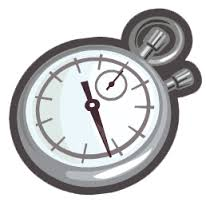
\includegraphics[width=0.75\marginparwidth]{stopwatch}
  \large\bf Opdracht \arabic{nstopdracht}}
}{%
  \end{minipage}
}

\newcounter{menucount}\newcounter{curitem}% Counters
\newcommand{\menuitem}{\texttt}% Menu item formatting
\newcommand{\menusep}{\ensuremath{\rightarrow}}% Menu separator
\newcommand{\menuend}{\relax}% Menu end
\newcommand{\menulist}[1]{% \menulist{<menu list>}
  \setcounter{menucount}{0}\setcounter{curitem}{0}% Reset menucount & curitem
  \renewcommand*{\do}[1]{\stepcounter{menucount}}%
  \menulistparser{#1}% Count menu items
  \renewcommand*{\do}[1]{\menuitem{##1}\stepcounter{curitem}\ifnumless{\value{curitem}}{\value{menucount}}{\menusep}{\menuend}}%
  \menulistparser{#1}% Process list
}
\DeclareListParser{\menulistparser}{:}% List separator is ':'


\begin{document}

\thispagestyle{empty}
\begin{center}
  \begin{mdframed}
  \centering
  \fontsize{40}{60}\selectfont Beschrijvende statistiek
  \end{mdframed}
  \vfill
  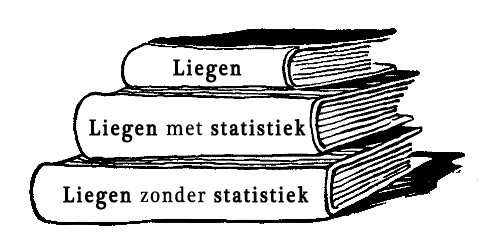
\includegraphics[width=0.8\textwidth]{statistiek_hoe_liegen}
  \vfill
\end{center}
\vfill
\subsection*{Doelstellingen}
{\singlespacing
Je kan \hfill (LP 2005-069, LI 2.3.1, ET14, ET15, ET17)
\begin{itemize}
  \item het onderscheid maken tussen een steekproef en een populatie,
  \item het gemiddelde en de mediaan berekenen van statische gegevens,
  \item de interkwartielafstand en de standaardafwijking berekenen van statistische gegevens,
  \item grafische voorstellingen maken van statistische gegevens,
  \item ICT gebruiken bij de drie voorgaande doelstellingen,
  \item aan de hand van voorbeelden het belang uitleggen van de representativiteit van een steekproef voor het formuleren van statische besluiten over de populatie, hierbij functioneel gebruik maken van centrummaten, spreidingsmaten en grafische voorstellingen,
  \item kritisch omgaan met het gebruik van statistiek in de media.
\end{itemize}
}

\thispagestyle{empty}
\newpage
\thispagestyle{empty}
\tableofcontents
\newpage
\clearpage
\pagenumbering{arabic}
\pagestyle{fancy}
\lhead{}

\fancyhead[RO,LE]{Beschrijvende statistiek}
\fancyhead[RE,LO]{}

\section{Begrip beschrijvende statistiek}

Met beschrijvende statistiek gaan we gegevens die we bekomen door tellen, waarnemen of enquêtes kort gaan weergeven of grafisch voorstellen. Het weergeven wordt vaak gedaan met behulp van {\em kengetallen} en het grafisch voorstellen met behulp van een aantal verschillende grafieken.

Welke kengetallen we gebruiken en welke grafieken we tekenen hangt af van de bekomen gegevens en hoe volledig die gegevens zijn. De gegevens worden steeds verzameld na het stellen van een {\bf onderzoeksvraag}. Er wordt dan dezelfde enquête of meting uitgevoerd bij een aantal personen of objecten, die we de {\bf elementen} zullen noemen. Elke eigenschap die we bevragen of meten noemen een {\bf variabele}.

\begin{oefening}
Noteer bij elke onderzoeksvraag de {\bf elementen} en de {\bf veranderlijke}:
\begin{enumerate}[(a)]
  \item Met welk vervoersmiddel komen de leerlingen naar onze school?
  \arules{2}
  \item Welke is het meest geliefde vak van alle laatstejaars leerlingen in Vlaanderen?
  \arules{2}
  \item Wat is het B.M.I. (body mass index) van de Belgen?
  \arules{2}
  \item Hoeveel computers zijn er per leerling beschikbaar voor gans Avelgem?
  \arules{2}
\end{enumerate}
\end{oefening}

\begin{oefening}
Geef zelf een onderzoeksvraag, de bijhorende elementen en veranderlijke. Maak hier een enquête voor op.
\end{oefening}

\pagebreak
\section{Populatie en steekproef}

De {\bf populatie} van een statistisch onderzoek is de verzameling van alle personen of objecten die bestudeerd worden. Als we bijvoorbeeld onderzoeken met welk vervoersmiddel onze leerlingen naar school komen, dan is de populatie alle leerlingen van onze school.

Meestal is het onmogelijk of moeilijk om de hele populatie te onderzoeken. We beperken ons dan tot een deelverzameling van de hele populatie. Deze noemen we de {\bf steekproef}. Om aan alle leerlingen van onze school te vragen welk vervoersmiddel ze gebruiken zouden we te veel tijd verliezen. Daarom kunnen we er bijvoorbeeld voor kiezen om maar aan een klein deel, bijvoorbeeld elke tiende leerlingen die door de schoolpoort komt te vragen hoe ze naar school gekomen zijn.

Een steekproef moet {\bf representatief} (ze moet een juist beeld geven van de populatie, alle deelgroepen moeten namelijk evenredig vertegenwoordigd zijn, {\bf aselect} (elk element van de populatie moet dezelfde kans hebben om opgenomen te worden tot de steekproef) en {\bf groot genoeg} zijn. Deze grootte noemen we de {\bf steekproefgrootte} $n$.

\begin{oefening}
Hoe zou je ervoor kunnen zorgen dat we een goede steekproef hebben van alle leerlingen van onze school?
\arules{3}
\end{oefening}


\begin{oefening}
Noteer van de volgende onderzoeken telkens de populatie, de steekproef en de steekproefgrootte.
\begin{enumerate}[(a)]
  \item Een interviewer vraagt telefonisch aan 500 Vlamingen of ze voor of tegen nieuwe verkiezingen zijn.
  \begin{itemize}
    \itemsep0.5em
    \item Populatie: \arulefill
    \item Steekproef: \arulefill
    \item Steekproefgrootte: \arulefill
  \end{itemize}
  \item Na elke rit in de Ronde van Frankrijk wordt een aantal renners onderzocht op doping.
  \begin{itemize}
    \itemsep0.5em
    \item Populatie: \arulefill
    \item Steekproef: \arulefill
    \item Steekproefgrootte: \arulefill
  \end{itemize}
\end{enumerate}
\end{oefening}

De eigenschap die we bestuderen noemen we de {\bf variabele}. Soms is dit een getal, bijvoorbeeld het aantal kilometer dat een leerling van school af woont, of soms niet, bijvoorbeeld het vervoersmiddel dat een leerlingen gebruikt om naar school te komen. We onderscheiden soorten variabelen die dan nog onderverdeeld zijn elk in twee soorten:
\begin{itemize}
  \item {\bf Kwalitatieve variabelen}
  \begin{itemize}
    \item {\bf Nominaal}: De verschillende waarden die een variabele heeft zijn niet zinvol te vergelijken.\\
    Bijvoorbeeld: Het vervoersmiddel van de leerling naar school (Te voet, Bus, Fiets, ...)
    \item {\bf Ordinaal}: De verschillende waarden die een variabele heeft kunnen geordend worden, we kunnen dus vergelijkingen maken zoals 'goed', 'beter', 'best'.\\
    Bijvoorbeeld: De tevredenheid van een televisieprogramma (*, **, ***, ****)
  \end{itemize}
  \item {\bf Kwantitatieve variabelen}
  \begin{itemize}
    \item {\bf Discreet}: De waarden zijn numeriek en bevatten onderbrekingen.\\
    Bijvoorbeeld: Het aantal gezinsleden (1, 2, 3, ...), de punten op een toets (..., 5, 5.5, 6, ...)
    \item {\bf Continue}: De waarden zijn numeriek, tussen een bepaald interval, en bevatten (minstens theoretisch) geen onderbrekingen. We kunnen dus de nauwkeurigheid zelf kiezen.\\
    Bijvoorbeeld: De afstand dat een leerling woont van school kan gegeven worden in kilometer, meter, centimeter, millimeter, ... Dus zo nauwkeurig als de onderzoeker zelf wenst.
  \end{itemize}
\end{itemize}

\begin{oefening}
Geef bij de volgende veranderlijken aan of het kwalitatieve of kwantitatieve veranderlijken zijn. Geef ook telkens één voorbeeld van een aantal mogelijke waarden.
\begin{center}
\begin{tabular}{p{6cm}|p{4cm}|p{4cm}}
Veranderlijke & Soort & Waarden\\
\hline
De smaak van fruitsnoepjes. & \arulefill & \arulefill[2]\\
Het aantal tv-toestellen dat Vlaamse gezinnen bezitten. & \arulefill & \arulefill[2]\\
De mate van tevredenheid bij klanten van een supermarkt. & \arulefill & \arulefill[2]\\
De afstand die leerlingen moeten afleggen als ze naar school komen. & \arulefill & \arulefill[2]\\
\end{tabular}
\end{center}
\end{oefening}

\pagebreak
\section{Kwalitatief onderzoek}

Heel vaak krijgen we in een onderzoek een aantal verschillende waarden van een variabele die niet zinvol te vergelijken is, namelijk een nominale variabele. Zo werd er vorig jaar aan een aantal leerlingen gevraagd met welk vervoersmiddel ze naar school kwamen, volgende dataset kregen we terug:
\begin{center}
fiets, bus, bus, auto, fiets, te voet, auto, te voet, fiets, fiets, auto, te voet, te voet, bus, bus, bus, auto, te voet, te voet, fiets, bus, bus, fiets, auto, te voet, skate board, te voet, fiets, fiets, bus, auto, bus, bus, bus, fiets, bus, te voet, te voet, fiets, auto, fiets, fiets, bus, te voet, bus, bus, fiets, bus, te voet, auto, te voet, fiets, bus, bus, bus, fiets, te voet, bus, fiets, fiets, bus 
\end{center}

In een {\bf dataset} is het de gewoonte om de $n$ waarneming te labelen met $x_1$, $x_2$, \ldots, $x_n$. Een aantal waarnemingen kunnen meerdere keren voorkomen, zo is $x_1=x_5=\ldots=x_{60}=$'fiets'. We maken die waarnemingen uniek door deze te labelen met $\omega_1=$'fiets' en deze krijgt dan de frequentie $n_1=17$


\subsection{Frequentietabel bij een kwalitatieve variabele}

Om vlot met deze data te kunnen werken maken we hier een {\bf frequentietabel} van, dit wil zeggen dat we de data in een tabel met op elke rij een unieke {\bf waarneming} en met de kolommen:
\begin{itemize}
  \item {\bf Waarnemingen} $\omega_j$: De unieke waarnemingen.
  \item {\bf Turven}: Manier van tellen waarbij we voor elke keer dat een waarneming voorkomt een verticaal streepje zetten, maar voor elke vijfde eenheid een groep van vier streepjes diagonaal doorhalen.
  \item {\bf Absolute frequentie} $n_j$: Aantal keren dat de waarneming voorkomt.
  \item {\bf Relatieve frequentie} $f_j$: Verhouding van de absolute frequentie van $\omega_j$ tot de steekproefgrootte $n$.\\
  Berekening: $$f_j=\dfrac{n_j}{n}$$
\end{itemize}

\begin{oefening}
Als er $k$ unieke waarnemingen $\omega_1, \omega_2, \ldots, \omega_k$ zijn, wat is dan de waarde van
$$f_1 + f_2 + \cdots f_k$$
\end{oefening}

\begin{oefening}
Maak de frequentietabel horende bij de dataset:
\begin{center}
fiets, bus, bus, auto, fiets, te voet, auto, te voet, fiets, fiets, auto, te voet, te voet, bus, bus, bus, auto, te voet, te voet, fiets, bus, bus, fiets, auto, te voet, skate board, te voet, fiets, fiets, bus, auto, bus, bus, bus, fiets, bus, te voet, te voet, fiets, auto, fiets, fiets, bus, te voet, bus, bus, fiets, bus, te voet, auto, te voet, fiets, bus, bus, bus, fiets, te voet, bus, fiets, fiets, bus 
\end{center}
\begin{center}
  \begin{tabular}{p{4cm}|p{3cm}|p{2.5cm}|p{2.5cm}}
    Waarneming $\omega_i$ & Turven & Frequentie $n_i$ & Rel. Freq. $f_i$\\
    \hline
    &&\\
    \hline
    &&\\
    \hline
    &&\\
    \hline
    &&\\
    \hline
    &&\\
    \hline
    &&\\
    \hline
    &&\\
    \hline
    &&\\
  \end{tabular}
\end{center}
\end{oefening}


\begin{oefening}
In september werd aan alle leerlingen van het derde jaar gevraagd of ze een rekentoestel hadden, en zo ja, van welk merk. Vervolledig de frequentietabel.
\begin{center}
\begin{tabular}{l|c|c}
Rekenmachine & Frequentie & Rel. Freq\\\hline
Geen & & 0.54\\\hline
Casio & 27 & 0.18\\\hline
TI & &\\\hline
n= & &\\
\end{tabular}
\end{center}
\end{oefening}

\pagebreak
\subsection{Grafische voorstellingen bij een kwalitatieve variabele}

\subsubsection{Staafdiagram}

Om de absolute frequentie van een kwalitatieve variabele grafisch weer te geven wordt vaak gebruik gemaakt van een staafdiagram. Op de $x$-as worden de verschillende optredende waarden van de waarnemingsgetallen gezet. Op de $y$-as wordt de overeenstemmende absolute frequentie geplaatst. Hoewel er bij een kwalitatieve variabele geen natuurlijke orde is wordt er geopteerd om steeds te ordenen van de grootste frequentie naar de kleinste frequentie. Er wordt ook afgesproken om de absolute frequentie boven elk staafje te schrijven. De staafjes mogen niet tegen elkaar staan.

Als voorbeeld zie je hier een staafdiagram
van de Vlaamse bevolking per provincie. De
informatie die hier wordt weergegeven, kan
je vinden in het boekje “Vlaanderen in
cijfers” op de website:
\url{http://www4.vlaanderen.be/dar/svr/Cijfers/Pages/Excel.aspx}.

  
\begin{minipage}{0.5\textwidth}
De namen van de provincies zijn afgekort als:
  \begin{description}
    \item[Antw] Antwerpen,
    \item[O-Vl] Oost-Vlaanderen,
    \item[W-Vl] West-Vlaanderen,
    \item[Vl-Br] Vlaams - Brabant,
    \item[Limb] Limburg.
  \end{description}
\end{minipage}
\begin{minipage}{0.5\textwidth}
%  \definecolor{qqqqff}{rgb}{0,0,1}
\begin{tikzpicture}[scale=0.1,line cap=round,line join=round,>=triangle 45,x=1.0cm,y=1.0cm]
\draw[-,color=black] (-9.63,0) -- (78.66,0);
\draw[color=black] (60,0.13) node [anchor=south west] { Provincie};
\draw[-,color=black] (0,-4.46) -- (0,27.9);
\draw[color=black] (0.57,27.25) node [anchor=west] { Aantal inwoners};
\clip(-9.63,-4.46) rectangle (78.66,27.9);
\draw[fill=black,fill opacity=0.1] (7,0) rectangle (12.5,8.39);
\draw[fill=black,fill opacity=0.1] (12.5,0) rectangle (17.5,0);
\draw[fill=black,fill opacity=0.1] (17.5,0) rectangle (22.5,10.77);
\draw[fill=black,fill opacity=0.1] (22.5,0) rectangle (27.5,0);
\draw[fill=black,fill opacity=0.1] (27.5,0) rectangle (32.5,11.59);
\draw[fill=black,fill opacity=0.1] (32.5,0) rectangle (37.5,0);
\draw[fill=black,fill opacity=0.1] (37.5,0) rectangle (42.5,14.32);
\draw[fill=black,fill opacity=0.1] (42.5,0) rectangle (47.5,0);
\draw[fill=black,fill opacity=0.1] (47.5,0) rectangle (52.5,17.45);
\draw (48.1,-0.39) node[anchor=north west] {Antw};
\draw (18.33,-0.43) node[anchor=north west] {Vl-Br};
\draw (28.4,-0.43) node[anchor=north west] {W-Vl};
\draw (38.13,-0.43) node[anchor=north west] {O-Vl};
\draw (7.91,-0.36) node[anchor=north west] {Limb};
\draw (46.85,24) node[anchor=north west] {1744862};
\draw (16.74,18) node[anchor=north west] {1076924};
\draw (26.93,12.35) node[anchor=north west] {1159366};
\draw (36.66,15.08) node[anchor=north west] {1432326};
\draw (7.23,9.13) node[anchor=north west] {838505};
\begin{scriptsize}
\fill [color=qqqqff] (0,0) circle (1.5pt);
\end{scriptsize}
\end{tikzpicture}

  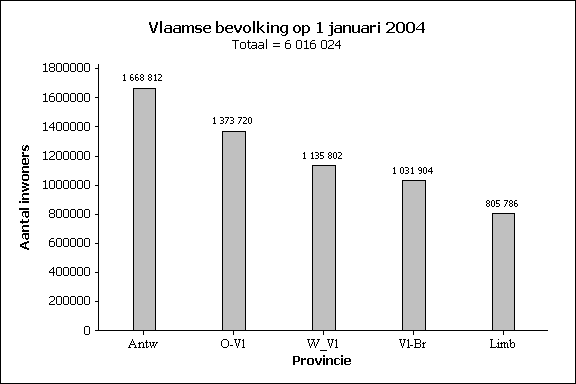
\includegraphics[width=8cm]{vlaamse_bevolking.png}
\end{minipage}

\begin{oefening}

\begin{minipage}{0.4\textwidth}
Gebruik de frequentietabel:
\begin{center}
  \begin{tabular}{c|c|c}
    $\omega_i$ & $n_i$ & $f_i$\\
    \hline
    fiets      & 17    & 0.28\\
    bus        & 21    & 0.34\\
    auto       &  8    & 0.13\\
    te voet    & 14    & 0.23\\
    skate board&  1    & 0.02
  \end{tabular}
\end{center}
\vspace*{1cm}
Om een staafdiagram te maken:
\end{minipage}
\begin{minipage}{0.6\textwidth}
\begin{center}
\assenstelsel[0.5]{-1}{20}{-1}{22}
\end{center}
\end{minipage}
\end{oefening}

\begin{oefening}
Aan 24 studenten werd gevraagd om een even getal tussen 0 en 9 te noemen en daarbij werd de volgende reeks getallen geregistreerd:
$$2 \qquad 6 \qquad 4 \qquad 0 \qquad 6 \qquad 8 \qquad 6 \qquad 4 \qquad 2 \qquad 4 \qquad 0 \qquad 6$$
$$8 \qquad 0 \qquad 0 \qquad 2 \qquad 4 \qquad 6 \qquad 8 \qquad 4 \qquad 0 \qquad 2 \qquad 2 \qquad 0$$
Maak de frequentietabel en teken het staafdiagram.
\end{oefening}

\subsubsection{Schijfdiagram}

Een {\bf schijfdiagram} of {\bf taartdiagram} is een grafische voorstelling van de relatieve frequenties.Bij het tekenen van een taartdiagram verdeel je een cirkeloppervlak in stukken, juist zoals je een
taart in stukken snijdt. Eén zo'n stuk heet een {\bf sector}. De totale oppervlakte van de cirkel komt overeen
met de som van alle percentages en dat is 100\%.

Voor een taartdiagram maken we enkele afspraken:
\begin{itemize}
  \item Begin bovenaan en draai met de wijzers van de klok mee.
  \item De grootste sector komt eerst, dan komt de tweede
grootste, enzovoort.
\end{itemize}


Je ziet hier een voorbeeld van de marktaandelen van
energiebevoorraders in België. Het gaat over de elektriciteit in
het jaar 2004. Deze figuur staat in het weekblad Knack van 22
juni 2005 en is goed leesbaar. Maar als je een krant of
weekblad doorbladert, dan zie je soms verwarrende en zelfs
verkeerde grafieken.

\begin{center}
  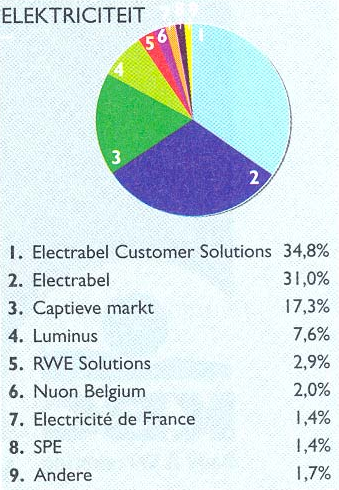
\includegraphics[width=0.4\textwidth]{cirkeldiagram_electriciteit}
\end{center}

Hoeveel graden elke sector is, bereken je door de relatieve
frequentie te vermenigvuldigen met $360\degree$. Dit doe je met je
rekenmachine. Maak daarna “verstandige” afrondingen zodat
alle sectoren samen terug $360\degree$ geven (je kan
eventueel enkele keren tot op een halve graad werken).

\begin{oefening}

\begin{minipage}{0.5\textwidth}
Gebruik de frequentietabel:
\begin{center}
  \begin{tabular}{c|c|c|c}
    $\omega_i$ & $n_i$ & $f_i$ & hoek\\
    \hline
    fiets      & 17    & 0.28  & \arule{1cm}\\
    bus        & 21    & 0.34  & \arule{1cm}\\
    auto       &  8    & 0.13  & \arule{1cm}\\
    te voet    & 14    & 0.23  & \arule{1cm}\\
    skate board&  1    & 0.02  & \arule{1cm}\\
  \end{tabular}
\end{center}
\vspace*{1cm}
Om een cirkeldiagram te maken:
\end{minipage}
\begin{minipage}{0.6\textwidth}
\begin{center}
\begin{tikzpicture}[scale=0.75,line cap=round,line join=round,>=triangle 45,x=1.0cm,y=1.0cm]
\draw(5,5) circle (5cm);
\draw (5,5)-- (5,10);
\end{tikzpicture}
\end{center}\end{minipage}
\end{oefening}

\begin{oefening}
We vragen aan een aantal mensen wat hun lievelingskleur is en krijgen volgende antwoorden:
\begin{center}
  rood, paars, groen, rood, groen, geel, purper, oranje, hemelsblauw, groen, rood, paars, geel, geel, zwart, groen, lichtgroen, oranje, geel, rood, oranje, groen, geel, groen, geel, blauw, rood, groen, oranje, blauw, rood, geel, groen, rood, paars, groen, rood, rood, blauw, geel, rood
\end{center}
Maak een taartdiagram.
\end{oefening}

\pagebreak
\subsection{Kwalitatief onderzoek in de media}

\begin{oefening}

Soms kom je de uitdrukking “horizontaal staafdiagram” tegen. Kijk daarvoor naar de figuur
die je vindt in de Gazet van Antwerpen van 3 november 2004. Voor de 364 jobs die in
oktober 2004 bij de 4 grootste faillissementen in Vlaanderen verloren gingen, heeft men een
figuur getekend.

\begin{center}
  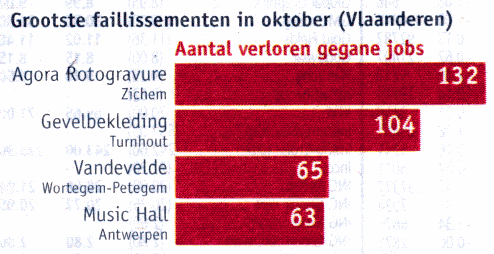
\includegraphics[width=0.6\textwidth]{horizontaal_staafdiagram-faillissementen}
\end{center}


\begin{itemize}
\item Welke veranderlijke is er genoteerd bij elke persoon die zijn job is kwijtgeraakt?
\arules{1}
\item Welk soort veranderlijke is dat?
\arules{1}
\item Wat zijn haar waarden?
\arules{2}
\item Is de figuur goed getekend?
\arules{2}
\end{itemize}
\end{oefening}

\begin{oefening}

Als je een frequentietabel ziet, dan moet je die juist kunnen interpreteren. Bekijk de tabel over XTC en Speed (Gazet van Antwerpen van 20-10-2004). Kijk enkel naar de informatie die daarin staat over het jaar 2003.

\begin{center}
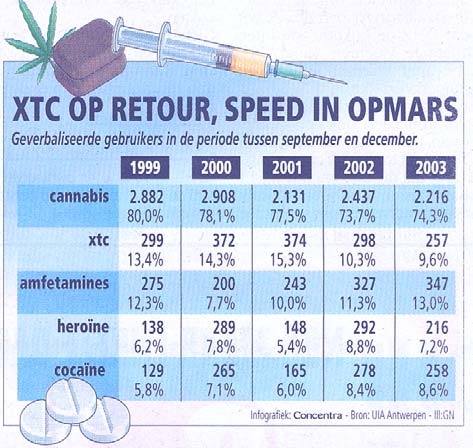
\includegraphics[width=0.7\textwidth]{tabel-drugs}
\end{center}

\begin{itemize}
  \item Is “druggebruik” daar behandeld als een kwalitatieve veranderlijke?
  \arules{2}
  \item Is de tabel correct?
  \arules{3}
\end{itemize}
\end{oefening}

\begin{oefening}
Een bestaande figuur moet je juist kunnen interpreteren. Bekijk het taartdiagram over de
vrijetijdsbesteding van jongeren (De Standaard van 6-12-2000).

\begin{center}
  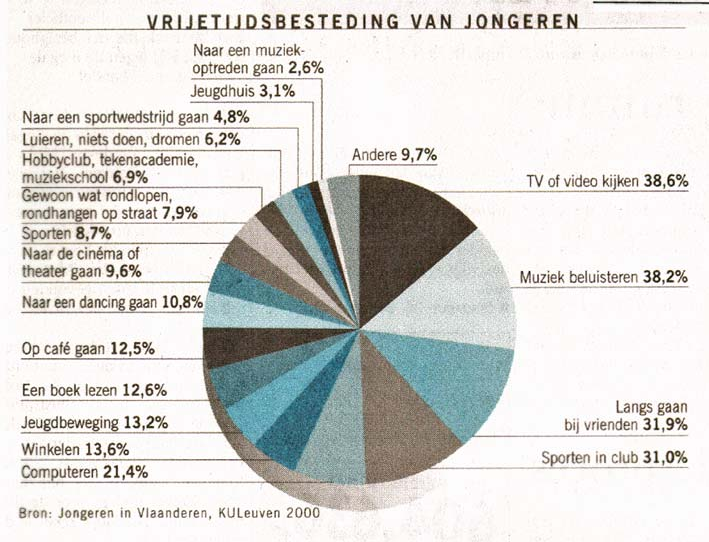
\includegraphics[width=1\textwidth]{cirkeldiagram-vrijetijdsbesteding}
\end{center}

\begin{itemize}
  \item Is “vrijetijdsbesteding” hier behandeld als een kwalitatieve veranderlijke?
  \arules{3}
  \item Is het taartdiagram correct getekend?
  \arules{3}
\end{itemize}
\end{oefening}

\pagebreak
\section{Kwantitatief onderzoek}

We herinneren ons dat we met een kwantitatieve variabele kunnen rekenen. We beschouwen nu een voorbeeld waarbij de directeur een aantal jaar terug de tijd heeft opgemeten dat het duurt voordat de leerling aan de les beginnen nadat het belsignaal heeft gerinkeld. We krijgen een lijst van 65 getallen waarbij elk getal een tijdstip in seconden voorstelt:

193, 225, 256, 166, 143, 260, 117, 208, 182, 114, 113, 203, 320, 231, 221, 231, 60, 113, 373, 180, 379, 205, 161, 287, 196, 236, 163, 192, 184, 166, 332, 172, 227, 272, 264, 155, 296, 189, 119, 230, 253, 225, 194, 200, 91, 177, 208, 157, 243, 183, 89, 235, 190, 223, 186, 132, 235, 312, 125, 258, 98, 173, 165, 289, 262


\subsection{Een frequentietabel met klassenindeling}

Je beschikt nu over een groot aantal opmetingen van een continu kwantitatieve veranderlijke. In feite is
elke geschatte tijdsduur verschillend van elke andere, maar daarvoor had je moeten meten tot op een
miljardste van een seconde (of misschien nog preciezer!). Als elke “echte” waarde verschillend is
van elke andere, dan komt elke “echte” waarde slechts één keer voor. Een frequentietabel zou dan
(theoretisch) al die verschillende “echte” waarden moeten bevatten, allemaal met een frequentie
gelijk aan één. Dat is zinloos.

De tijdsmetingen die je hier hebt, worden, zoals alle continue veranderlijken, samengevat in een
{\bf frequentietabel met klassenindeling}.

\begin{center}
  \begin{tabular}{|c|c|}
    \hline
    Klasse & Frequentie\\
    \hline
    $[60;65[$ & $1$\\    
    \hline
    $[65;70[$ & $0$\\
    \hline
    $[70;75[$ & \ldots\\ 
    \hline
    \ldots & \ldots\\ 
    \hline
  \end{tabular}
\end{center}

Voor het maken van de klassen kan je als volgt te werk gaan.
\begin{itemize}
  \item Start met een interval dat groot genoeg is om al je opmetingen te kunnen bevatten. Als je
kleinste observatie 60 is en je grootste is 379, dan moet je dus minstens van 60 tot 379 gaan.
Meestal neem je eenvoudige “ronde” getallen. Hier zou je bijvoorbeeld kunnen starten bij 60 en eindigen bij 380 of 390 (13 keer een halve minuut).
  \item Op dit grote interval maak je nu deelintervallen die mooi aan elkaar aansluiten en elkaar niet overlappen. Dat zijn je klassen. De breedte van die klassen mag je zelf kiezen en ze hoeven zelfs niet allemaal even breed te zijn.
  \item Elke klasse is een “links gesloten – rechts open” interval, zoals bijvoorbeeld $[60;65[$. De grenzen van een klasse heten {\bf klassengrenzen}. Het midden heet {\bf klassenmidden} en de breedte heet {\bf klassenbreedte}.
  \item Zorg ervoor dat het overgrote deel van de waarnemingen niet binnen één of twee klassen valt. Als richtlijn neem je tussen de 5 en de 15 klassen, maar deze richtlijn hoef je niet te strikt te nemen. Als je de frequentietabel gebruikt om een histogram te tekenen (zoals uitgelegd in volgend puntje), dan zal je ervaren dat te veel klassen dikwijls een zeer onrustige figuur geven terwijl te weinig klassen bijna niets meer tonen.
\end{itemize}

Als de tabel gemaakt is, dan kan het turven beginnen. {\bf Turven} is tellen door streepjes per vijf te groeperen. Dit doe je door de elementen van je dataset te overlopen en voor elk element een streepje te plaatsen bij de correcte klasse.

%\vfill
\begin{center}
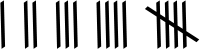
\includegraphics[width=0.3\textwidth]{turven}
\end{center}

%\newpage
\begin{oefening}
Stel nu een frequentietabel voor de volgende dataset. Kies een verstandige klassenbreedte.\\
193, 225, 256, 166, 143, 260, 117, 208, 182, 114, 113, 203, 320, 231, 221, 231, 60, 113, 373, 180, 379, 205, 161, 287, 196, 236, 163, 192, 184, 166, 332, 172, 227, 272, 264, 155, 296, 189, 119, 230, 253, 225, 194, 200, 91, 177, 208, 157, 243, 183, 89, 235, 190, 223, 186, 132, 235, 312, 125, 258, 98, 173, 165, 289, 262
\\
\begin{center}
  \setlength{\tabcolsep}{5pt}
  \renewcommand{\arraystretch}{1}
  \begin{tabular}{|p{2cm}|p{2cm}|p{2cm}|p{2cm}|p{2cm}|p{2cm}|}
    \hline
    Klasse & Turf & Frequentie &&Relatieve Frequentie&\\
    \hline&&&&&\\\hline&&&&&\\\hline&&&&&\\\hline&&&&&\\\hline&&&&&\\
    \hline&&&&&\\\hline&&&&&\\\hline&&&&&\\\hline&&&&&\\\hline&&&&&\\
    \hline&&&&&\\\hline&&&&&\\\hline
  \end{tabular}
\end{center}
\end{oefening}

Naast de frequentie en de relatieve frequentie bestaan er ook nog de {\it cumulatieve} versies van deze frequenties. Cumulatief wil zeggen dat iets steeds toeneemt of ophoopt. In het geval van de frequentie is de {\bf cumulatieve frequentie} het aantal gegevens dat tot deze klasse en alle lagere klassen behoord. De {\bf relatieve cumulatieve frequentie} van een klasse is dan de verhouding van de cumulatieve frequentie van die klasse en het totale aantal gegevens.

Vul de frequentietabel verder aan met de cumulatieve frequentie en de relatieve cumulatieve frequentie.

\begin{oefening}
Gemiddeld is een basketbal speler $2.01 \m$ groot. Op de website van de (National Basketball Association) NBA vinden we volgende dataset.\\

1.93, 2.22, 2.08, 2.26, 1.98, 2.13, 2.16, 1.94, 1.89, 1.96, 1.92, 2.09, 2.11, 2.09, 2.13, 2, 1.67, 2.08, 2.2, 2.18, 2.18, 2.17, 1.96, 1.95, 2.01, 2.07, 1.74, 1.81, 2.04, 1.99, 1.99, 1.91, 1.74, 2.12, 1.95, 2, 2.25, 2.29, 1.9, 1.98, 2.03, 2.16, 1.82, 2.17, 1.92, 1.99, 1.95, 2, 2, 1.91, 2.26, 2.21, 2.31, 1.91, 2.1, 2.09, 2.17, 1.98, 1.95, 1.96, 2.21, 2.18, 1.96, 1.82, 1.89, 2.21, 2.09, 1.87, 1.83, 2.16, 1.87, 2.18, 2.09, 2.1, 1.7, 2.01, 2.2, 1.67, 1.87, 2.14\\

Maak een goede frequentietabel.
\end{oefening}

\begin{oefening}
In een klas met 24 leerlingen geef ik een onverwachte toets op 10. Volgende resultaten werden behaald en op score geplaatst:\\

7.5, 9, 9, 5.5, 8.5, 7.5, 7, 9, 7.5, 3, 8.5, 6, 8, 8.5, 7.5, 8, 9, 7, 9, 7, 7, 8, 6, 8\\

Maak een goede frequentietabel.
\end{oefening}

\pagebreak
\subsection{Het histogram}

Een {\bf histogram} is de meest gebruikte figuur om het globale gedrag van continu
kwantitatieve gegevens te onderzoeken. Deze stelt de frequentieverdeling bij klassenindeling
grafisch voor. We maken een histogram als volgt:

\begin{enumerate}
  \item Kies op de $x$-as een lengte-eenheid en breng op de $x$-as de beeldpunten van de klassengrenzen aan. Elke klasse komt dan overeen met een lijnstuk.
  \item De klassenfrequenties worden voorgesteld met behulp van rechthoeken die de horizontale lijnstukken op de $x$ as als zijde hebben. Dan moet de verticale zijde zo zijn, dat de oppervlakte van de bijbehorende rechthoek recht evenredig is met de frequentie van een klasse. We moeten dus de hoogte van elke rechthoek berekenen en vervolgens die rechthoeken construeren, allen aan de zelfde kant van de $x$-as.
\end{enumerate}

Vaak zal men boven het histogram ook nog een {\bf frequentiepolygoon} tekenen. Hierbij verbind men het hoogste punt van de staafjes binnen het histogram in het klassenmidden met elkaar. Soms wordt voor de kleinste waarde en na de grootste waarde nog twee fictieve waarden toevoegen, elk met frequentie nul, zodat de frequentiepolygoon begint en eindigt op de $x$-as.

\begin{oefening}
Teken het histogram en het frequentiepolygoon horende bij volgende frequentietabel.\\
\begin{minipage}{0.5\textwidth}
\begin{center}
\begin{tabular}{c|c|c|c}
$i$ & klasse     & $n_i$ & $f_i$\\
\hline
  1 & $[ 60,  90[$ &   2 &  0.03\\
  2 & $[ 90, 120[$ &   7 &  0.11\\
  3 & $[120, 150[$ &   3 &  0.05\\
  4 & $[150, 180[$ &  10 &  0.15\\
  5 & $[180, 210[$ &  16 &  0.25\\
  6 & $[210, 240[$ &  11 &  0.17\\
  7 & $[240, 270[$ &   7 &  0.11\\
  8 & $[270, 300[$ &   4 &  0.06\\
  9 & $[300, 330[$ &   2 &  0.03\\
 10 & $[330, 360[$ &   1 &  0.02\\
 11 & $[360, 390[$ &   2 &  0.03\\
\end{tabular}
\end{center}
\end{minipage}
\begin{minipage}{0.6\textwidth}
\begin{center}
\assenstelsel[0.6]{-1}{13}{-1}{17}
\end{center}
\end{minipage}
\end{oefening}


\subsubsection*{Verschil tussen een staafdiagram en een histogram}
Sommigen denken dat een histogram en een staafdiagram goed op elkaar
lijken. Dat is fout, want er zijn fundamentele verschillen. Een histogram hoort
bij een continu kwantitatieve veranderlijke waar geen tussenstappen zijn tussen
de “mogelijke” uitkomsten. Bij een histogram liggen de rechthoeken dus tegen
elkaar. Bij een staafdiagram is er open ruimte tussen de staafjes. Bovendien
kijk je bij een staafdiagram naar de hoogte en bij een histogram naar de
oppervlakte.

\begin{oefening}
Als je de groottes van de basketbalspelers in acht klassen hebt opgedeeld krijgen we volgende frequentietabel. Maak zelf het bijhorende histogram en teken het frequentiepolygoon.\\
\begin{minipage}{0.5\textwidth}
\begin{center}
\begin{tabular}{c|c|c}
$i$ & klasse     & $n_i$\\
\hline
  1 & $[ 1.60,  1.70[$ &   2\\
  2 & $[ 1.70,  1.80[$ &   3\\
  3 & $[ 1.80,  1.90[$ &   9\\
  4 & $[ 1.90,  2.00[$ &   22\\
  5 & $[ 2.00,  2.10[$ &   16\\
  6 & $[ 2.10,  2.20[$ &   17\\
  7 & $[ 2.20,  2.30[$ &   10\\
  8 & $[ 2.30,  2.40[$ &   1\\
\end{tabular}
\end{center}
\end{minipage}
\begin{minipage}{0.6\textwidth}
\begin{center}
\assenstelsel[0.7]{-1}{10}{-1}{14}
\end{center}
\end{minipage}
\end{oefening}

\begin{oefening}
In een klas met 24 leerlingen geef ik een onverwachte toets op 10. Volgende resultaten werden behaald en op score geplaatst:
\begin{center}
7.5, 9, 9, 5.5, 8.5, 7.5, 7, 9, 7.5, 3, 8.5, 6, 8, 8.5, 7.5, 8, 9, 7, 9, 7, 7, 8, 6, 8
\end{center}
Maak frequentietabel en een staafdiagram.
\end{oefening}



\pagebreak
\subsection{Numerieke kenmerken: de kengetallen}

Jij en je buur kunnen elkaars punten van het rapport vergelijken. Elke reeks punten van een rapport kan je zien als een reeks waarnemingsgetallen. Hiervan zou je bijvoorbeeld elkaars gemiddelde kunnen vergelijken of hoe de punten verspreid liggen.

Je zou ook een onderzoek kunnen doen naar lichaamsgrootte binnen een aantal verschillende sporten. Je kan bijvoorbeeld 100 basketters interviewen en 150 volleybalspelers. Van de bekomen reeksen van klassen kunnen we ook weer bepaalde {\bf kengetallen} berekenen. We zullen onderscheid maken tussen centrummaten en spreidingsmaten.

\subsubsection{Centrummaten}

{\bf Centrummaten} geven de waarde waarrond de waarnemingsgetallen gecentreerd zijn. Ze tonen ons het midden van de data.

De ons best gekende is het {\bf gemiddelde} $\bar{x}$. Bij een reeks van $n$ waarnemingsgetallen $x_1$, $x_2$, $\ldots$, $x_n$ berekenen we het gemiddelde met
$$\bar{x}=\dfrac{x_1 + x_2 + \cdots + x_n}{n}$$
We kunnen dit korter schrijven als
$$\bar{x}=\dfrac{1}{n}\sum^n_{i=1}x_i$$
Als we een indeling in klassen hebben kunnen we niet langer het gemiddelde exact bepalen. We berekenen dan een schatting als volgt:
\begin{enumerate}
  \item Bereken van alle klassen het klassenmidden.
  \item Bereken het product van het klassenmidden met de frequentie.
  \item Bepaal de som van de voorgaande producten.
  \item Deel deze som door de steekproefgrootte $n$.  
\end{enumerate}

\begin{oefening}
Bepaal het gemiddelde van de volgende toetsresultaten:
\begin{center}
7.5, 9, 9, 5.5, 8.5, 7.5, 7, 9, 7.5, 3, 8.5, 6, 8, 8.5, 7.5, 8, 9, 7, 9, 7, 7, 8, 6, 8
\end{center}
\end{oefening}

\begin{oefening}
Bepaal het gemiddelde van de volgende frequentietabel
\begin{center}
\begin{tabular}{c|c|c}
$i$ & klasse     & $n_i$\\
\hline
  1 & $[ 1.60,  1.70[$ &   2\\
  2 & $[ 1.70,  1.80[$ &   3\\
  3 & $[ 1.80,  1.90[$ &   9\\
  4 & $[ 1.90,  2.00[$ &   22\\
  5 & $[ 2.00,  2.10[$ &   16\\
  6 & $[ 2.10,  2.20[$ &   17\\
  7 & $[ 2.20,  2.30[$ &   10\\
  8 & $[ 2.30,  2.40[$ &   1\\
\end{tabular}
\end{center}
\end{oefening}

De volgende centrummaat is de {\bf mediaan} Med, dit is het getal zodat er evenveel getallen kleiner dan of gelijk zijn aan de mediaan als dat er getallen groter dan of gelijk zijn aan de mediaan. Bij een reeks waarnemingsgetallen berekenen we de mediaan als volgt $x_1$, $x_2$, $\ldots$, $x_n$:
\begin{itemize}
  \item $n$ is oneven: We nemen het middelste getal na het ordenen van de getallen.
  \item $n$ is even: We nemen het gemiddelde van de twee middelste getallen na het ordenen van de getallen.
\end{itemize}
Als we een indeling in klassen hebben nemen we het klassenmidden (of het gemiddelde van de klassenmiddens bij een even steekproefgrootte) van de klasse waar de middelste waarneming zich bevind. Merk op dat het interessant is om hiervoor de kolom met cumulatieve frequenties te gebruiken.

\begin{oefening}
Bepaal de mediaan van de volgende toetsresultaten:
\begin{enumerate}[(a)]
  \item 7.5, 9, 9, 5.5, 8.5, 7.5, 7, 9, 7.5, 3, 8.5, 6, 8, 8.5, 7.5, 8, 9, 7, 9, 7, 7, 8, 6, 8
  \item 7.5, 9, 9, 5.5, 8.5, 7.5, 7, 9, 7.5, 3, 8.5, 6, 8, 8.5, 7.5, 8, 9, 7, 9, 7, 7, 8, 6, 8, 3
\end{enumerate}
\end{oefening}

\begin{oefening}
Bepaal de mediaan van de volgende frequentietabelen
\begin{multicols}{2}
\begin{enumerate}[(a)]
  \item 
  \begin{center}
\begin{tabular}{c|c|c}
$i$ & klasse     & $n_i$\\
\hline
  1 & $[ 1.60,  1.70[$ &   2\\
  2 & $[ 1.70,  1.80[$ &   3\\
  3 & $[ 1.80,  1.90[$ &   9\\
  4 & $[ 1.90,  2.00[$ &   22\\
  5 & $[ 2.00,  2.10[$ &   16\\
  6 & $[ 2.10,  2.20[$ &   17\\
  7 & $[ 2.20,  2.30[$ &   10\\
  8 & $[ 2.30,  2.40[$ &   1\\
\end{tabular}
\end{center}
  \item 
  \begin{center}
\begin{tabular}{c|c|c}
$i$ & klasse     & $n_i$\\
\hline
  1 & $[ 1.60,  1.70[$ &   2\\
  2 & $[ 1.70,  1.80[$ &   3\\
  3 & $[ 1.80,  1.90[$ &   9\\
  4 & $[ 1.90,  2.00[$ &   22\\
  5 & $[ 2.00,  2.10[$ &   17\\
  6 & $[ 2.10,  2.20[$ &   17\\
  7 & $[ 2.20,  2.30[$ &   10\\
  8 & $[ 2.30,  2.40[$ &   1\\
\end{tabular}
\end{center}
\end{enumerate}
\end{multicols}
\end{oefening}

Tot slot is er nog de {\bf modus} Mod. Bij een reeks waarnemingsgetallen $x_1$, $x_2$, $\ldots$, $x_n$ is dat de waarneming die het meeste voorkomt. Als er meerdere waarneming de hoogste frequentie hebben is de modus een verzameling van deze waarnemingsgetallen. Bij een indeling in klassen nemen we de klassen met de hoogste frequentie als als modus, we noemen deze dan de {\bf modale klasse}.

We merken verder op dat het gemiddelde veel gevoeliger is dan de mediaan. Wat we hiermee bedoelen is dat, indien er in een reeks waarnemen extreme waarden voorkomen die eigenlijk onmogelijk zouden zijn, dat het gemiddelde hierdoor beïnvloed wordt. De mediaan kan dus soms een betere centrummaat zijn.

\begin{oefening}
In een fabriek worden 1 liter flessen gevuld met ketjup. Om te controleren dat er geen fout zit op de machine wordt er elk uur steekproefgewijs 8 flessen gewogen. We krijgen volgende data de maandagmorgen:
\begin{center}
  230 gr; 1202 gr; 1212 gr; 1183 gr; 1191 gr; 1236 gr; 1232 gr; 1193 gr 
\end{center}
\begin{enumerate}[(a)]
  \item Bepaal het gemiddelde.
  \item Bepaal de mediaan.
  \item Welke centrumwaarde past hier het best bij de data en waarom?
\end{enumerate}
\end{oefening}

\pagebreak
\subsubsection{Spreidingsmaten}

Met {\bf spreidingsmaten} kunnen we met getallen weergeven hoe de waarnemingsgetallen verspreid liggen rond een centrummaat. Beschouw bijvoorbeeld volgende twee datasets
\begin{center}
  4\; 6\; 8\; 10 \qquad\qquad en \qquad\qquad 1\; 4\; 5\; 9\; 11\; 12
\end{center}
Beide reeksen hebben hetzelfde gemiddelde en dezelfde mediaan. Toch is er een verschil, namelijk de linker dataset ligt dichter ronde het gemiddelde en de mediaan dan de rechter dataset. We zeggen dat de spreiding links kleiner is.

De eenvoudigste spreidingsmaat is de {\bf variatiebreedte} $R$. Deze geeft ons de afstand tussen het kleinste en grootste getal van een reeks waarnemingen $x_1$, $x_2$, $\ldots$, $x_n$:
$$R=\max_{i=1}^n x_i - \min_{i=1}^n x_i $$
Bij een indeling in klassen wordt de afstand tussen de kleinste en grootste klassenmidden berekend.

\begin{oefening}
Bepaal de variatiebreedte van volgende waarnemingsgetallen:
\begin{center}
7.5, 9, 9, 5.5, 8.5, 7.5, 7, 9, 7.5, 3, 8.5, 6, 8, 8.5, 7.5, 8, 9, 7, 9, 7, 7, 8, 6, 8
\end{center}
\end{oefening}

\begin{oefening}
Bepaal de variatiebreedte van de volgende frequentietabel
\begin{center}
\begin{tabular}{c|c|c}
$i$ & klasse     & $n_i$\\
\hline
  1 & $[ 1.60,  1.70[$ &   2\\
  2 & $[ 1.70,  1.80[$ &   3\\
  3 & $[ 1.80,  1.90[$ &   9\\
  4 & $[ 1.90,  2.00[$ &   22\\
  5 & $[ 2.00,  2.10[$ &   16\\
  6 & $[ 2.10,  2.20[$ &   17\\
  7 & $[ 2.20,  2.30[$ &   10\\
  8 & $[ 2.30,  2.40[$ &   1\\
\end{tabular}
\end{center}
\end{oefening}

\pagebreak
Een weinig gebruikte spreidingsmaat is de {\bf gemiddelde absolute afwijking} $Mad$ die de gemiddelde afstand van een reeks waarnemingsgetallen $x_1$, $x_2$, $\ldots$, $x_n$ bepaalt:
$$Mad=\dfrac{1}{n}\sum_{i=1}^n|x_i-\bar{x}|$$

Wij laten deze buiten beschouwing daar deze in de praktijk toch niet gebruikt wordt. Wel vaak gebruikt zijn de {\bf variatie} $s^2$ die het gemiddelde van het kwadraat van de afstanden van een reeks waarnemingen $x_1$, $x_2$, $\ldots$, $x_n$ bepaalt:
$$s^2=\dfrac{1}{n}\sum_{i=1}^n(x_i-\bar{x})^2$$
Door het kwadraat krijgen we echter een vertekeningen, daarom werd de {\bf standaardafwijking} $s$ ingevoerd:
$$s=\sqrt{\dfrac{1}{n}\sum_{i=1}^n(x_i-\bar{x})^2}$$

Om bij een indeling in klassen de variatie en standaardafwijking te berekenen gebruiken we opnieuw de producten die bekomen worden door het klassenmidden te vermenigvuldigen met de frequentie. We verkiezen echter om deze kengetallen te berekenen met het \zrm{ZRM}.

Een andere maat voor spreiding is de lengte van het gebied waarin de middelste 50\% van de
geordende opmetingen liggen. Dit gebied loopt van het {\bf eerste kwartiel} $Q_1$ tot het {\bf derde kwartiel} $Q_3$.
De lengte van dit interval is de {\bf interkwartielafstand}, genoteerd als $IQR$ (= InterQuartile Range).
Als we de reeds berekende mediaan $Q_2$ noemen, dan is $Q_1$ te bepalen door de mediaan te nemen van de
gegevens links van $Q_2$ en $Q_3$ is te bepalen door de mediaan te nemen van de gegevens rechts van $Q_2$. Ook
dit kengetal zullen we berekenen met software.

\subsubsection{Berekenen van de 1-variabele statistieken}

Alle voorgaande kengetallen vatten we samen met de {\bf 1-variabele statistieken}. Deze kunnen allemaal
in één keer berekend worden met het \zrm{ZRM}. De instructies zijn afhankelijk van het rekentoestel. Ook geeft het nieuwe rekentoestel iets meer kengetallen. Het verschil is echter niet groot, een nieuwer rekentoestel heb je zeker niet nodig voor de oefeningen.

\begin{minipage}{\textwidth}
\begin{multicols}{2}

\begin{center}
  \begin{mdframed}Nieuw model: fx-92B Spéciale Collège\end{mdframed}
\end{center}\mbox{}\\
Kies \zrm{MENU} en daarna \zrm{2:Statistics} en \zrm{EXE}. Nu kan de juiste soort statistische variabele, \zrm{1:1-Variable} gekozen worden waarna alle waarnemingen ingevoerd kunnen worden. Kies daarna het \zrm{OPTN} en \zrm{3:1-Variable Calc}.

\vfill\columnbreak

\begin{center}
  \begin{mdframed}Oud model: fx-92B Collège 2D+\end{mdframed}
\end{center}\mbox{}\\
Kies \zrm{MODE} en daarna \zrm{2:STAT} en \zrm{EXE}. Nu kan de juiste soort statistische variabele, \zrm{1:1-VAR} gekozen worden waarna alle waarnemingen ingevoerd kunnen worden. Druk daarna op \zrm{AC}. Nu ben je in rekengedeelte van de statistiek mode. De \verb#0# die daar staat is normaal. Nu kan je de verschillende statistieken uitrekenen met \zrm{SHIFT} \zrm{STAT} (bij het knopje van 1). Kies daar \zrm{4:Var} en dan \zrm{2:$\bar{x}$} voor gemiddelde of \zrm{3:s$x$} voor de standaard afwijking.

\end{multicols}
\end{minipage}

De volgende zijn belangrijk:
\begin{center}
  \begin{tabular}{r|l}
    $\bar{x}$ & Het gemiddelde.\\
    $s^2x$ & De variatie.\\
    $sx$ & De standaard afwijking.\\
    $n$ & De steekproefgrootte.\\
    $min(x)$ & De laagste waarde.\\
    $Q_1$ & Het eerste kwartiel.\\
    $Med$ & De mediaan.\\
    $Q_3$ & Het derde kwartiel.\\
    $max(x)$ & De hoogste waarde.\\
  \end{tabular}
\end{center}

\begin{oefening}
Bepaal de 1-variabele statistieken van volgende waarnemingsgetallen m.b.v. het \zrm{ZRM}:
\begin{center}
7.5, 9, 9, 5.5, 8.5, 7.5, 7, 9, 7.5, 3, 8.5, 6, 8, 8.5, 7.5, 8, 9, 7, 9, 7, 7, 8, 6, 8
\end{center}
\end{oefening}

\pagebreak
\subsection{De boxplot}

\begin{wrapfigure}[10]{l}{0.4\textwidth}
  \vspace{-1cm}
  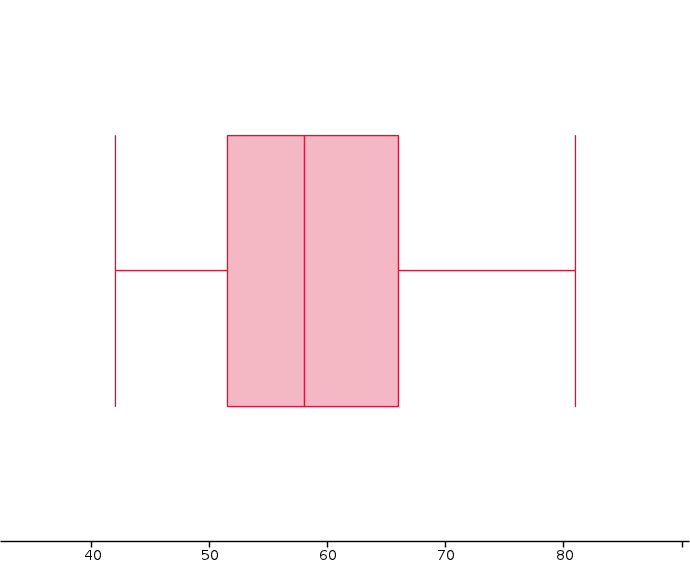
\includegraphics[width=0.4\textwidth]{boxplot}
\end{wrapfigure}

Een goed zicht op zowel het centrum als de spreiding van je opmetingen, krijg je uit een boxplot. Dit
is een grafiek die gebruik maakt van de begrippen minimum, maximum, mediaan, eerste kwartiel
Q1, derde kwartiel Q3, IQR en uitschieters.

De rechterstaart begint vanaf Q3. Dit lijnstuk gaat tot aan de grootste opmeting die kleiner of
gelijk is aan $\mbox{Q3} + (1.5\cdot\mbox{IQR})$. Elke observatie die nog groter is, wordt als een uitschieter
beschouwd en apart aangeduid. In deze studie loopt de rechterstaart van $66$ tot $81$ en heeft
dus een lengte van $15$. Op een analoge manier teken je de linkerstaart, links van Q1. Die
loopt hier van $42$ tot $51.5$, wat een lengte van $9.5$ oplevert.
De rechthoekjes duiden aan waar de middelste getallen van de dataset liggen. De
linkerrechthoek gaat van Q1 tot Med. In dat gebied ligt het tweede kwart van de geordende
getallen. De rechterrechthoek gaat van Med tot Q3, en daar ligt het derde kwart van deze
getallen.

\begin{oefening}
Teken de boxplot voor volgende waarnemingsgetallen:
\begin{enumerate}[(a)]
  \item 7.5, 9, 9, 5.5, 8.5, 7.5, 7, 9, 7.5, 3, 8.5, 6, 8, 8.5, 7.5, 8, 9, 7, 9, 7, 7, 8, 6, 8
  \item 7.5, 9, 9, 5.5, 8.5, 7.5, 7, 9, 7.5, 3, 8.5, 6, 22, 8, 8.5, 7.5, 8, 9, 7, 9, 7, 7, 8, 6, 8
\end{enumerate}
\end{oefening}

\pagebreak
\section{Extra oefeningen}

\begin{oefening}
Wanneer is een kwantitatieve veranderlijke continu? Zeg dat in je eigen woorden, en geef
enkele voorbeelden.
\end{oefening}

\begin{oefening}
Schrijf je een continu kwantitatieve veranderlijke altijd op met kommagetallen? Motiveer je
antwoord.
\end{oefening}

\begin{oefening}
Welke eigenschap probeert de standaardafwijking te beschrijven? Zeg in woorden hoe je de
standaardafwijking berekent. Kan je daaruit afleiden of de standaardafwijking gevoelig is
voor uitschieters? Kan je daarvan een eenvoudig voorbeeld geven?
\end{oefening}

\begin{oefening}
Welke eigenschap probeert de interkwartielafstand te beschrijven? Zeg in woorden wat
kwartielen zijn en hoe je de interkwartielafstand berekent. Kan je daaruit afleiden of de
interkwartielafstand gevoelig is voor uitschieters? Kan je daarvan een eenvoudig voorbeeld
geven?
\end{oefening}

\pagebreak
\section{Voorbeeld examenvragen}

\paragraph{Vraag 1}
Van de {\em sweet \& fair shop} krijg je de volgende dataset\footnote{Met dank aan de studenten van 6SETA.}:

druivensuiker aardbei; druivensuiker mango; kinderrozijnen; amandel chocolades; zure frieten; zure frieten; coco-mango reep; koban mix; kinderrozijnen; druivensuiker mango; zure frieten; kinderrozijnen;  druivensuiker mango; druivensuiker aardbei;  druivensuiker mango; druivensuiker mango; druivensuiker mango; druivensuiker aardbei; druivensuiker aardbei; druivensuiker aardbei; druivensuiker aardbei; kinderrozijnen;

Stel een frequentietabel op:
\begin{center}
  \begin{tabular}{p{4cm}|p{4cm}|p{4cm}}
    &absolute frequentie&relatieve frequentie\\
    \hline
    &&\\[6cm]
  \end{tabular}
\end{center}

Wat heb je genomen als veranderlijke? \arulefill
Dit is een kwalitatieve/kwantitatieve veranderlijke. {\tiny (schrappen wat niet past)}
Wat is de steekproefgrootte? \arulefill
Er zijn twee manieren om de data grafisch voor te stellen, welke:
\begin{itemize}
  \item \arule{6cm}
  \item \arule{6cm}
\end{itemize}

\newpage
Stel je data grafisch voor (op twee manieren)

\ruitjes{20cm}

\newpage
\paragraph{Vraag 2}
Aan een aantal studenten uit het eerste jaar hoger onderwijs werd gevraagd hoeveel auto's er bij hen in het gezin waren. De data die we terugkregen was als volgt:
2; 0; 3; 1; 1; 1; 3; 1; 1; 1; 2; 1; 0; 0; 2; 0; 0; 0; 7; 1; 2; 2; 2; 2; 1; 1; 1; 2; 2; 3

Wat zijn de elementen in dit onderzoek?
\arules{1}

Welke veranderlijke wordt hier onderzocht?
\arules{1}

Waarom mag je zeggen dat de veranderlijke in dit onderzoek kwantitatief is?
\arules{2}

Is de kwantitatieve veranderlijke discreet of continue?
\arules{1}

Vervolledig de frequentietabel (het is niet nodig om de data in klassen op te delen):
\begin{center}
  \setlength{\tabcolsep}{7pt}
  \renewcommand{\arraystretch}{1.5}
  \begin{tabular}{p{4cm}|p{4cm}|p{4cm}}
    &&\\
    \hline
    0&&\\
    1&&\\
    2&&\\
    3&&\\
    4&&\\
    5&&\\
    6&&\\
    7&&\\
    &n=&\\
  \end{tabular}
\end{center}

Maak een histogram waarin je absolute frequenties gebruikt.

\begin{center}
\definecolor{cqcqcq}{rgb}{0.65,0.65,0.65}
\begin{tikzpicture}[xscale=1,yscale=0.3,line cap=round,line join=round,>=triangle 45,x=1.0cm,y=1.0cm]
\draw [color=cqcqcq,dash pattern=on 1pt off 1pt, xstep=1.0cm,ystep=1.0cm] (-1,-1) grid (12,12);
\draw[->,color=black] (-1,0) -- (12,0);
\draw[shift={(1,0)},color=black] (0pt,2pt) -- (0pt,-2pt) node[below] {\footnotesize $1$};
\draw[color=black] (0.25,12.07) node [anchor=south west] { x};
\draw[->,color=black] (0,-1) -- (0,12);
\draw[shift={(0,1)},color=black] (2pt,0pt) -- (-2pt,0pt) node[left] {\footnotesize $1$};
\draw[color=black] (12.09,-1.25) node [anchor=west] { y};
\draw[color=black] (0pt,-10pt) node[right] {\footnotesize $0$};
\end{tikzpicture}
\end{center}

Is het belangrijk de grootste absolute frequentie vooraan wordt geplaatst?
\arules{1}

In hoeveel gezinnen zijn er $4$ auto's? \arulefill
Waarom staat de waarde $4$ dan toch in de frequentietabel?
\arules{2}

Is het nuttig om ook in het histogram een plaatsje op de $x$-as te voorzien voor $4$ auto's, hoewel er daar geen staaf getekend is?
\arules{2}

Bereken het gemiddeld aantal auto's per gezin:
%\vspace*{1cm}
$$\bar{x}=\arule{5cm}$$

Voor wat is het gemiddelde gevoelig?
\arules{1}

Wat is de oplossing hierop?
\arules{1}

Geef deze voor ons voorbeeld:
\arules{1}

\newpage
\paragraph{Vraag 3}
Tijdens de opendeurdag laat de afdeling hout de leerlingen uit het zesde leerjaar planken zagen op 180 cm. Na tien planken meten we de reeds gezaagde planken en we vinden de volgende lengtes:\\
177; 178; 178; 179; 179; 180; 181; 181; 183; 184 cm\\

{\em Bereken of bepaal m.b.v. \zrm{ZRM} en geef ook steeds het correcte symbool!}

Steekproefgrootte:\arulefill

Gemiddelde:\arulefill

Standaard afwijking\footnote{$s = \sqrt{\frac{\mbox{som van alle gekwadrateerde afwijkingen t.o.v. het gemiddelde}}{n-1}} = \sqrt{\frac{\sum_{i=0}^n(\bar{x}-x_i)^2}{n-1}}$}:\arulefill

Maximum:\arulefill

Minimum:\arulefill

Eerste kwartiel:\arulefill

Mediaan:\arulefill

Derde kwartiel:\arulefill

Interkwartielafstand:\arulefill

Teken de boxplot:

\ruitjes{3cm}

\end{document}

\subsubsection*{Gemiddelde en mediaan}

Hoe de testpersonen de tijdsduur van 1 minuut geschat hebben is mooi weergegeven
in het histogram. Maar wat doe je als men vraagt om al die informatie in enkele
getallen samen te vatten?

Een samenvatting in getallen (die {\bf kengetallen} worden genoemd) geeft je zelden evenveel
informatie als een goede figuur. Maar soms kan een kengetal dienen als “typisch” resultaat. Dat is
natuurlijk wel handig.

Als eerste kenmerk wil je weten hoelang een typische proefpersoon denkt dat een minuut duurt.
Daarom ga je op zoek naar een getal dat “het centrum” van al je resultaten weergeeft. Een
gebruikelijk kengetal hiervoor is het {\bf gemiddelde}. Een ander kengetal voor “centrum” is de
{\bf mediaan}.

Deze kengetallen kunnen enkel berekend worden bij kwantitatieve gegevens.

Bij {\bf discrete kwantitatieve gegevens} wordt het gemiddelde berekend door het quotiënt te nemen van hun som en hun aantal. De mediaan wordt berekend door de gegevens te rangschikken van klein naar groot en het middelste getal te nemen als het aantal gegevens oneven is of het gemiddelde te nemen van de middelste twee getallen als het aantal getallen even is.

Een simpel voorbeeld is:

\begin{oefening}
Bereken het gemiddelde van de volgende toetsresultaten: 4, 5.5, 6, 6, 6, 6.5, 7, 7, 7, 7.5, 7.5, 8, 8, 8, 8, 8.5, 8.5, 9, 9.5, 10, 10.\\
\ruitjes{3cm}
\end{oefening}

\begin{oefening}
Bereken de mediaan van de volgende toetsresultaten: 4, 5.5, 6, 6, 6, 6.5, 7, 7, 7, 7.5, 7.5, 8, 8, 8, 8, 8.5, 8.5, 9, 9.5, 10, 10.\\
\ruitjes{3cm}
\end{oefening}

In het vorige voorbeeld werd het gemiddelde en mediaan berekend van discrete kwantitatieve gegevens. Ons
onderzoek bevat {\bf continue kwantitatieve gegevens} die gegroepeerd zijn in een frequentietabel. Om hiervan
het gemiddelde te berekenen zoeken we van elke klasse het {\bf klassenmidden}, dit is de halve som van de
ondergrens en de bovengrens van die klasse. Bijvoorbeeld van de klasse $[42, 46[$ is het klassenmidden
$$
\frac{42 + 46}{2}=44\;.
$$

Dit klassenmidden wordt nu vermenigvuldigd met elke frequentie. Dit noemen we het product. Alle bekomen producten worden opgeteld. Het gemiddelde is dan het quotiënt van som van de producten en de som van de frequenties.
\newpage

\begin{stopdracht}
Bereken nu het gemiddelde.
\begin{center}
  \setlength{\tabcolsep}{7pt}
  \renewcommand{\arraystretch}{1.5}
  \begin{tabular}{|p{2cm}|p{3cm}|p{2cm}|p{2cm}|}
    \hline
    Klasse & Klassenmidden & Frequentie & Product\\
    \hline&&&\\\hline&&&\\\hline&&&\\\hline&&&\\\hline&&&\\
    \hline&&&\\\hline&&&\\\hline&&&\\\hline&&&\\\hline&&&\\
    \hline&&&\\\hline&&&\\\hline&&&\\\hline&&&\\\hline&&&\\\hline
    \multicolumn{2}{r|}{Som:} & &\\\cline{3-4}
  \end{tabular}
\end{center}
\vspace*{0.5cm}
Het gemiddelde is:
$$
\bar{x}=\frac{\phantom{.......................}}{\phantom{.....................}}=
$$
\vspace*{0.5cm}
\end{stopdracht}
\vspace*{-0.5cm}

Omdat onze gegevens gegroepeerd zijn moeten we bij het berekenden van de mediaan de gegevens ordenen van klein naar groot en kijken in welke klasse de middelste waarde zich bevind. Hiervoor hebben we dus de ruwe data nodig. Deze sorteren we van klein naar groot. De middelste waarde bij een oneven aantal gegevens bepaald de klasse waar de mediaan in ligt. Het klassenmidden is dan de mediaan. Bij een even aantal gegevens bepaald het gemiddelde van de twee middelste gegevens de klasse. De mediaan is dan ook het klassenmidden van deze klassen.

\newpage
\begin{stopdracht}
Bepaal de mediaan van ons onderzoek.\\
\ruitjes{4cm}
\end{stopdracht}

\subsubsection*{Standaardafwijking en interkwartielafstand}

Om je opmetingen te karakteriseren is het “centrum” maar een eerste stap. Een tweede karakteristiek
is de spreiding rond dit centrum. De gebruikelijke kengetallen hiervoor zijn de standaardafwijking en
de interkwartielafstand. Zij worden ook {\bf spreidingsmaten} genoemd.

Om de spreiding van de gegevens rond het gemiddelde te berekenen, gebruik je de
{\bf standaardafwijking} $s$. Voor de standaardafwijking bestaat een “te gekke” formule. Die ziet eruit als
$$
s = \sqrt{\frac{1}{n-1}\sum^n_{i=1}(x_i - \bar{x})^2}
$$
waarbij $n$ staat voor het aantal gegevens, $\bar{x}$ voor het gemiddelde en $x_i$ voor het $i$-de gegeven. Dit kengetal zullen we straks berekenen met software.

Een andere maat voor spreiding is de lengte van het gebied waarin de middelste 50\% van de
geordende opmetingen liggen. Dit gebied loopt van het {\bf eerste kwartiel} Q1 tot het {\bf derde kwartiel} Q3.
De lengte van dit interval is de {\bf interkwartielafstand}, genoteerd als IQR (= InterQuartile Range).
Als we de reeds berekende mediaan Q2 noemen, dan is Q1 te bepalen door de mediaan te nemen van de
gegevens links van Q2 en Q3 is te bepalen door de mediaan te nemen van de gevens rechts van Q2. Ook
dit kengetal zullen we berekenen met software.

\subsubsection{Berekenen van de 1-variabele statistieken}

Alle voorgaande kengetallen vatten we samen met de {\bf 1-variabele statistieken}. Deze kunnen allemaal
in één keer berekend worden met Geogebra. Selecteer hiervoor de lijst met data en kies het icoon 
{\it onderzoek één variabele}. Verschuif het aantal klassen naar $10$. Geogebra zal het histogram plotten
een lijst geven met kengetallen.

De volgende zijn belangrijk:
\begin{center}
  \begin{tabular}{r|l}
    $n$ & Het aantal gegevens.\\
    Gemiddelde & Het rekenkundig gemiddelde.\\
    $s$ & De standaard afwijking.\\
    Min & De laagste waarde.\\
    Q1 & Het eerste kwartiel.\\
    Mediaan & De mediaan.\\
    Q3 & Het derde kwartiel.\\
    Max & De hoogste waarde.\\
  \end{tabular}
\end{center}

\begin{center}
  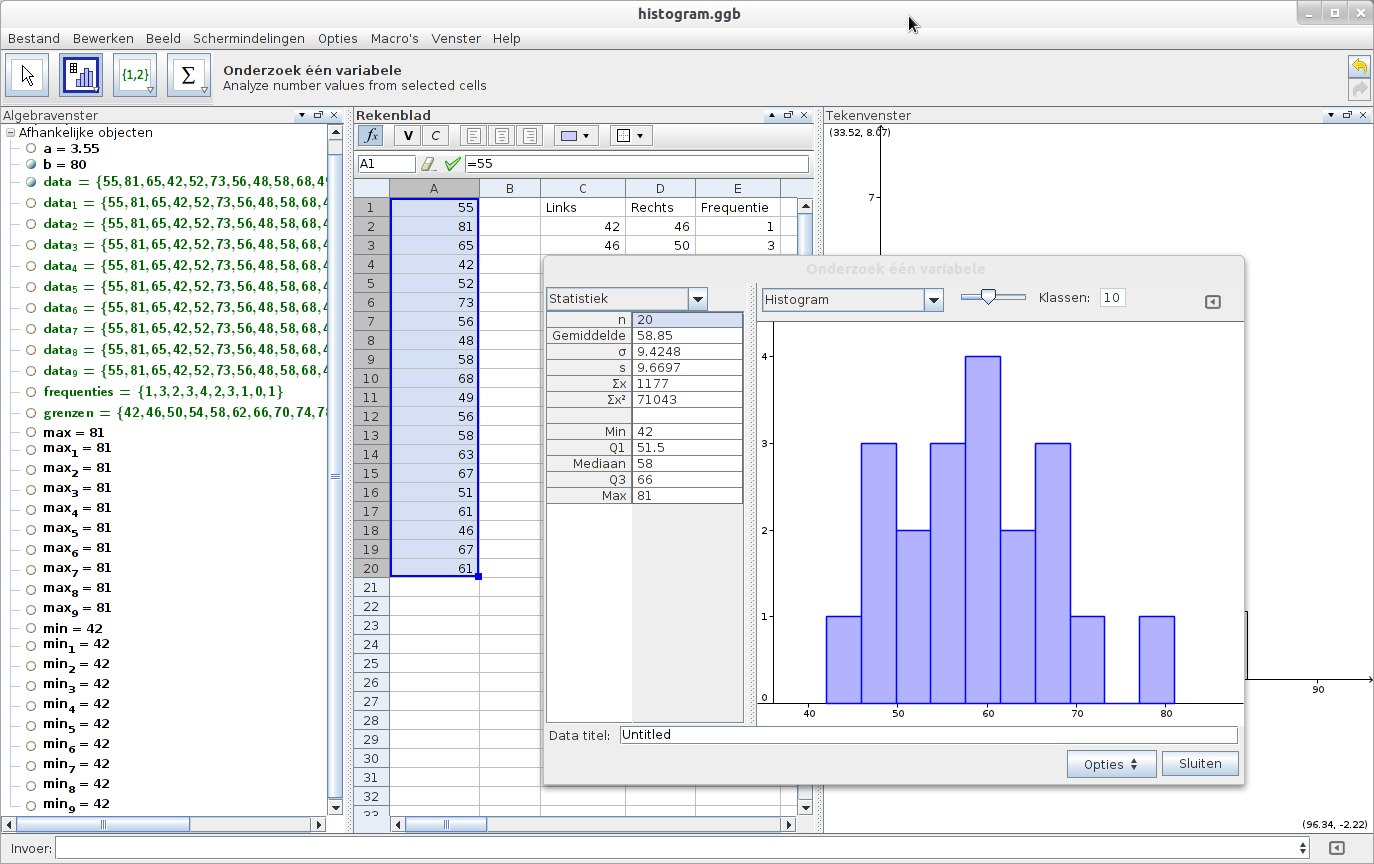
\includegraphics[width=14cm]{gg-1var_stat}
\end{center}

\subsubsection{De boxplot}

\begin{wrapfigure}[10]{l}{0.4\textwidth}
  \vspace{-1cm}
  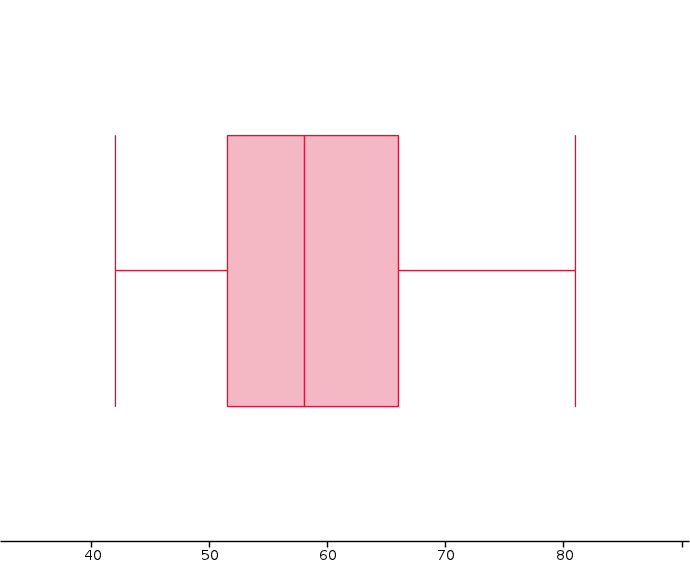
\includegraphics[width=0.4\textwidth]{boxplot}
\end{wrapfigure}

Een goed zicht op zowel het centrum als de spreiding van je opmetingen, krijg je uit een boxplot. Dit
is een grafiek die gebruik maakt van de begrippen minimum, maximum, mediaan, eerste kwartiel
Q1, derde kwartiel Q3, IQR en uitschieters.

De rechterstaart begint vanaf Q3. Dit lijnstuk gaat tot aan de grootste opmeting die kleiner of
gelijk is aan $\mbox{Q3} + (1.5\cdot\mbox{IQR})$. Elke observatie die nog groter is, wordt als een uitschieter
beschouwd en apart aangeduid. In deze studie loopt de rechterstaart van $66$ tot $81$ en heeft
dus een lengte van $15$. Op een analoge manier teken je de linkerstaart, links van Q1. Die
loopt hier van $42$ tot $51.5$, wat een lengte van $9.5$ oplevert.
De rechthoekjes duiden aan waar de middelste getallen van de dataset liggen. De
linkerrechthoek gaat van Q1 tot Med. In dat gebied ligt het tweede kwart van de geordende
getallen. De rechterrechthoek gaat van Med tot Q3, en daar ligt het derde kwart van deze
getallen.

\begin{stopdracht}
Teken nu de boxplot van het onderzoek. Vergeet de x-as niet te voorzien van de juiste getallen en de juiste eenheid.
\ruitjes{6cm}
\end{stopdracht}

\begin{stopdracht}
Zijn er uitschieters in je dataset? Was dat te verwachten?
\arules{3}
\end{stopdracht}

In Geogebra krijg je een boxplot door in het venster van de 1-variabele statistieken {\it Boxplot} te kiezen in plaats van {\it Histogram}.

\begin{center}
  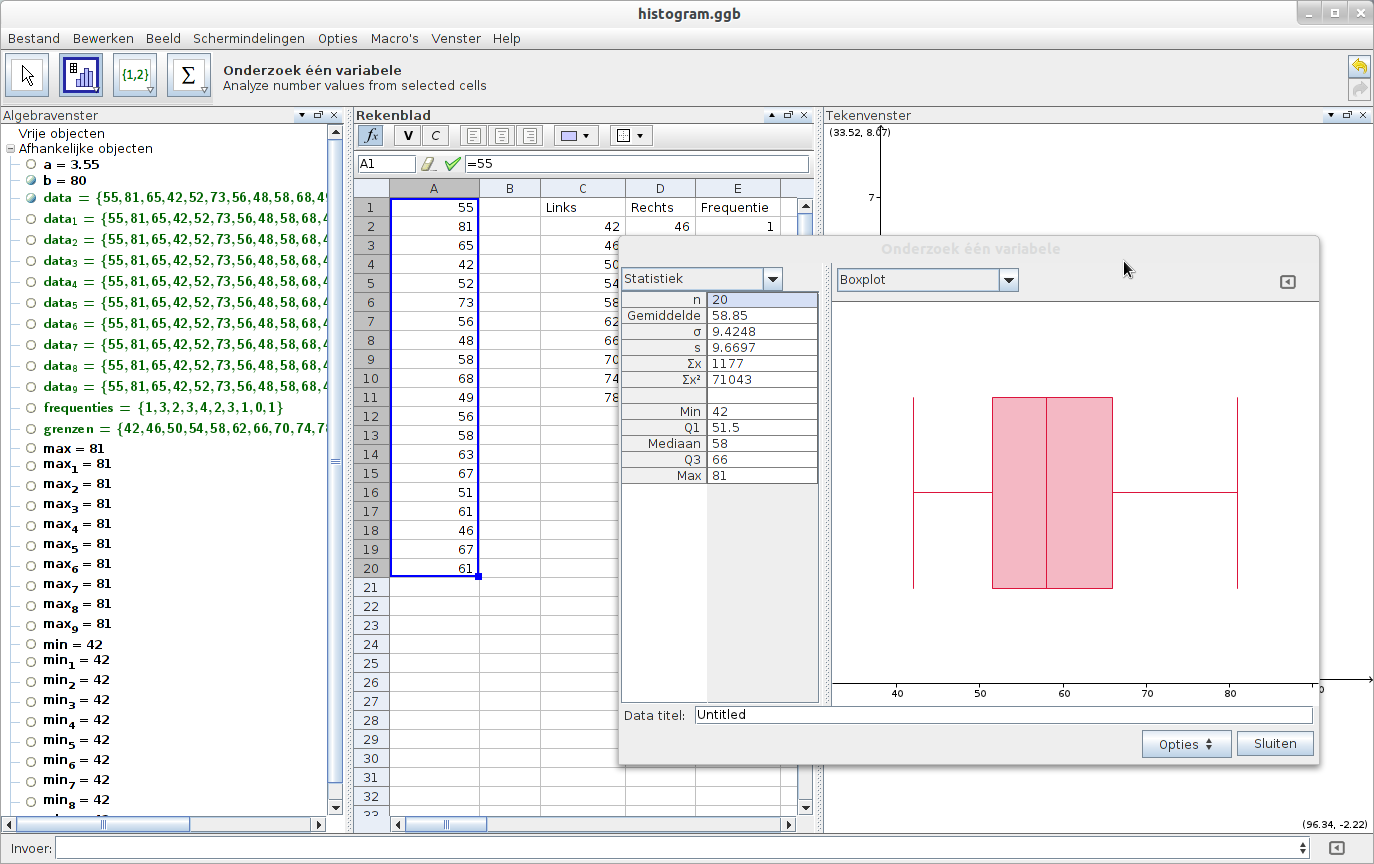
\includegraphics[width=14cm]{gg-boxplot}  
\end{center}

\subsection{Wat heb je gevonden? Hoever kan je gaan in je conclusie?}

\subsubsection{De variabiliteit van steekproefresultaten}

Je bent er nu al mee vertrouwd. Een steekproef levert toevallige resultaten op, en bij een andere
steekproef krijg je andere resultaten. Indien je de populatie van alle leerlingen van je school in
identieke omstandigheden de tijdsduur van één minuut zou laten schatten, dan zou het gemiddelde
van al die schattingen niet exact samenvallen met het gemiddelde dat jij in je steekproef hebt
gevonden. Dat is niet erg. De statistiek is er juist om je te helpen om goede uitspraken over de
populatie te doen. Als er tenminste geen andere problemen opduiken... .

In dit onderzoek heb je elke leerling aan een kleine test onderworpen. De manier waarop die test
moet worden afgenomen heb je vooraf heel precies vastgelegd, en je hebt je aan die procedure strikt
gehouden bij elke leerling die je hebt getest. Maar er is nog iets anders dat voor fouten kan zorgen.
Je werkt met meetapparatuur, en is die wel goed geijkt? Als je een chronometer gebruikt die start bij
2 in plaats van bij 0, dan heb je in al je opmetingen een systematische fout van 2 seconden. Je krijgt
dan een vertekend beeld van de werkelijkheid.

Als al je opmetingen op een systematische manier te klein (of te groot) zijn dan heb je {\bf vertekening}.
Vertekening in metingen kan je met statistiek niet opsporen. Je moet vooraf controleren of je
apparatuur wel juist geijkt is. Doe dit vooraleer je aan je onderzoek begint!

\begin{oefening}
Je moet de lengte van 20 planken meten en je doet dat met een rolmeter. Op welke manier
zou hier vertekening kunnen optreden?
\arules{3}
\end{oefening}

\begin{center}
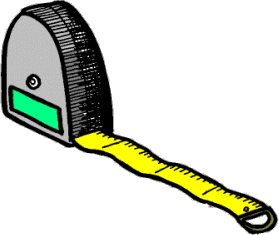
\includegraphics[width=5cm]{rolmeter}
\end{center}

\begin{oefening}
Soms kan je op een spitsvondige manier vertekening in opmetingen neutraliseren. Als je een
weegschaal moet gebruiken waarvan je vermoedt dat zij systematisch een te laag gewicht
aangeeft, hoe zou jij dan een boekentas daarop wegen, als je met die weegschaal vooraf niets
mag doen?
\ruitjes{7cm}
\end{oefening}

\subsubsection{Een uitspraak over de populatie}

Wat we in het “exploratief” onderzoek hebben gevonden is van toepassing op de dataset die we hebben
onderzocht, en dus op alle leerlingen van de klas. Als je op een goede manier een steekproef trekt, als je je
strikt houdt aan de procedure om de leerlingen te testen, en als je meetapparatuur goed geijkt is, dan
kan je met statistiek verantwoorde uitspraken doen over hoe heel de school een minuut zou schatten.
Voor deze steekproef was het gemiddelde $58.85$ seconden en de mediaan was $58$ seconden. Dat ligt
niet ver uit elkaar, en je zou kunnen vermoeden dat het gemiddelde en de mediaan van de hele
populatie ook wel in de buurt van $58$ seconden liggen. Waarschijnlijk is dat nog waar ook.

\subsection{Kernachtige samenvatting van dit onderzoek}

Je samenvatting bestaat uit twee delen
\begin{enumerate}
  \item De antwoorden op de contextvragen (de www-vragen),
  \item De besluiten over het uitgevoerde onderzoek.
\end{enumerate}

Betrek ook de kengetallen in je besluit: vermeld hun getalwaarde en ga na in hoever ze een zinvolle
karakteristiek zijn voor dit onderzoek. Vergeet ook nooit om goede grafieken te tekenen en die te
interpreteren.

\begin{stopdracht}
Formuleer nu de antwoorden op de contextvragen (de www-vragen).
\arules{8}
\end{stopdracht}

\begin{stopdracht}
Formuleer nu de besluiten over het uitgevoerde onderzoek.
\arules{8}
\end{stopdracht}

\newpage
\subsection{Zelfevaluatie}

In dit onderzoek heb je geleerd over:
\begin{itemize}
  \item vertekening bij opmetingen
  \item de continu kwantitatieve veranderlijke
  \item de frequentietabel met klassenindeling
  \item het histogram en de boxplot
  \item het gemiddelde en de mediaan
  \item de standaardafwijking en de interkwartielafstand
  \item de interpretatie van kengetallen in combinatie met grafieken
\end{itemize}

Je bent nu in staat om volgende opdrachten uit te voeren:

\begin{oefening}
Wanneer is een kwantitatieve veranderlijke continu? Zeg dat in je eigen woorden, en geef
enkele voorbeelden.
\arules{6}
\end{oefening}

\begin{oefening}
Schrijf je een continu kwantitatieve veranderlijke altijd op met kommagetallen? Motiveer je
antwoord.
\arules{6}
\end{oefening}

\begin{oefening}
Welke eigenschap probeert de standaardafwijking te beschrijven? Zeg in woorden hoe je de
standaardafwijking berekent. Kan je daaruit afleiden of de standaardafwijking gevoelig is
voor uitschieters? Kan je daarvan een eenvoudig voorbeeld geven?
\arules{6}
\end{oefening}

\begin{oefening}
Welke eigenschap probeert de interkwartielafstand te beschrijven? Zeg in woorden wat
kwartielen zijn en hoe je de interkwartielafstand berekent. Kan je daaruit afleiden of de
interkwartielafstand gevoelig is voor uitschieters? Kan je daarvan een eenvoudig voorbeeld
geven?
\arules{6}
\end{oefening}

\newpage
\section*{Voorbeeld examen}
\vraag{14}
Van de {\em sweet \& fair shop} krijg je de volgende dataset\footnote{Met dank aan de studenten van 6SETA.}:

druivensuiker aardbei; druivensuiker mango; kinderrozijnen; amandel chocolades; zure frieten; zure frieten; coco-mango reep; koban mix; kinderrozijnen; druivensuiker mango; zure frieten; kinderrozijnen;  druivensuiker mango; druivensuiker aardbei;  druivensuiker mango; druivensuiker mango; druivensuiker mango; druivensuiker aardbei; druivensuiker aardbei; druivensuiker aardbei; druivensuiker aardbei; kinderrozijnen;

Stel een frequentietabel op:
\begin{center}
  \begin{tabular}{p{4cm}|p{4cm}|p{4cm}}
    &absolute frequentie&relatieve frequentie\\
    \hline
    &&\\[6cm]
  \end{tabular}
\end{center}

Wat heb je genomen als veranderlijke? \arulefill
Dit is een kwalitatieve/kwantitatieve veranderlijke. {\tiny (schrappen wat niet past)}
Wat is de steekproefgrootte? \arulefill
Er zijn twee manieren om de data grafisch voor te stellen, welke:
\begin{itemize}
  \item \arule{6cm}
  \item \arule{6cm}
\end{itemize}

\newpage
Stel je data grafisch voor (op twee manieren)

\ruitjes{20cm}

\newpage
\vraag{16}
Aan een aantal studenten uit het eerste jaar hoger onderwijs werd gevraagd hoeveel auto's er bij hen in het gezin waren. De data die we terugkregen was als volgt:
2; 0; 3; 1; 1; 1; 3; 1; 1; 1; 2; 1; 0; 0; 2; 0; 0; 0; 7; 1; 2; 2; 2; 2; 1; 1; 1; 2; 2; 3

Wat zijn de elementen in dit onderzoek?
\arules{1}

Welke veranderlijke wordt hier onderzocht?
\arules{1}

Waarom mag je zeggen dat de veranderlijke in dit onderzoek kwantitatief is?
\arules{2}

Is de kwantitatieve veranderlijke discreet of continue?
\arules{1}

Vervolledig de frequentietabel (het is niet nodig om de data in klassen op te delen):
\begin{center}
  \setlength{\tabcolsep}{7pt}
  \renewcommand{\arraystretch}{1.5}
  \begin{tabular}{p{4cm}|p{4cm}|p{4cm}}
    &&\\
    \hline
    0&&\\
    1&&\\
    2&&\\
    3&&\\
    4&&\\
    5&&\\
    6&&\\
    7&&\\
    &n=&\\
  \end{tabular}
\end{center}

Maak een histogram waarin je absolute frequenties gebruikt.

\begin{center}
\definecolor{cqcqcq}{rgb}{0.65,0.65,0.65}
\begin{tikzpicture}[xscale=1,yscale=0.3,line cap=round,line join=round,>=triangle 45,x=1.0cm,y=1.0cm]
\draw [color=cqcqcq,dash pattern=on 1pt off 1pt, xstep=1.0cm,ystep=1.0cm] (-1,-1) grid (12,12);
\draw[->,color=black] (-1,0) -- (12,0);
\draw[shift={(1,0)},color=black] (0pt,2pt) -- (0pt,-2pt) node[below] {\footnotesize $1$};
\draw[color=black] (0.25,12.07) node [anchor=south west] { x};
\draw[->,color=black] (0,-1) -- (0,12);
\draw[shift={(0,1)},color=black] (2pt,0pt) -- (-2pt,0pt) node[left] {\footnotesize $1$};
\draw[color=black] (12.09,-1.25) node [anchor=west] { y};
\draw[color=black] (0pt,-10pt) node[right] {\footnotesize $0$};
\end{tikzpicture}
\end{center}

Is het belangrijk de grootste absolute frequentie vooraan wordt geplaatst?
\arules{1}

In hoeveel gezinnen zijn er $4$ auto's? \arulefill
Waarom staat de waarde $4$ dan toch in de frequentietabel?
\arules{3}

Is het nuttig om ook in het histogram een plaatsje op de $x$-as te voorzien voor $4$ auto's, hoewel er daar geen staaf getekend is?
\arules{2}

Bereken het gemiddeld aantal auto's per gezin:
%\vspace*{1cm}
$$\bar{x}=\arule{5cm}$$

Voor wat is het gemiddelde gevoelig?
\arules{1}

Wat is de oplossing hierop?
\arules{1}

Geef deze voor ons voorbeeld:
\arules{1}

\newpage
\vraag{10}
Tijdens de opendeurdag laat de afdeling hout de leerlingen uit het zesde leerjaar planken zagen op 180 cm. Na tien planken meten we de reeds gezaagde planken en we vinden de volgende lengtes:\\
177; 178; 178; 179; 179; 180; 181; 181; 183; 184 cm\\

{\em Bereken of bepaal en geef ook steeds het correcte symbool!}

Steekproefgrootte:\arulefill

Gemiddelde:\arulefill

Standaard afwijking\footnote{$s = \sqrt{\frac{\mbox{som van alle gekwadrateerde afwijkingen t.o.v. het gemiddelde}}{n-1}} = \sqrt{\frac{\sum_{i=0}^n(\bar{x}-x_i)^2}{n-1}}$}:\arulefill

Maximum:\arulefill

Minimum:\arulefill

Eerste kwartiel:\arulefill

Mediaan:\arulefill

Derde kwartiel:\arulefill

Interkwartielafstand:\arulefill

Teken de boxplot:

\ruitjes{3cm}

\end{document}

\newpage
\section{Projecten}

Kies één van volgende projecten om zelf een onderzoek rond uit te voeren:

\vraag{Je wenst als dierenarts te beginnen in een stad. Om te kunnen inschatten hoeveel
'klanten' je zal hebben wil je weten hoeveel huisdieren er ongeveer zijn in het dorp. Je
kan uiteraard niet bij iedereen langs gaan. Zet een onderzoek op om het totaal aantal
huisdieren in te schatten.}{1cm}


\vraag{Een fietsenmaker wenst voor de nieuwe collectie 20 MTB te kopen. Hij weet alleen
niet goed welke kleuren hij zou nemen. Hij weet dat jij reeds statistiek hebt gevolgd en vraagt
je raad. Hoe zul je dit aanpakken. Wat is de populatie, wat is een goede steekproef? Zal de
data bestaan uit kwantitatieve of kwalitatieve gegevens?}{1cm}

\vraag{De leesbaarheid van een tekst hangt onder meer af van de lengte van de zinnen. Korte zinnen
lezen gemakkelijker dan lange zinnen. Als je aanneemt dat zowat elke nieuwe zin met een
hoofdletter begint, en dat er verder niet te veel afkortingen in hoofdletters voorkomen, dan is
de verhouding van het aantal hoofdletters ten opzichte van het totale aantal letters een goede
maat voor de lengte van de zinnen. Het is nu aan jou om voor deze werktekst een goede schatting te
maken van de proportie hoofdletters. Hoe ga je dat doen? Is er een mogelijkheid om een getrapte
steekproef te nemen?}{1cm}

\vraag{Stel zelf een onderzoek op naar iets dat je interesseert. Bepaal eerst een goede
onderzoeksvraag. Bepaal daarna pas de populatie en geef dan een methode om een steekproef
te nemen.}{1cm}

Kijk steeds eerst wat je wilt weten en hoe je gaat meten. Onderzoek dan de dataset en trek je
conclusies. Geef op het einde een samenvatting van het onderzoek.

\end{document}

\begin{thebibliography}{1}
\bibitem{1}\label{1} Prof. dr. Herman Callaert, Hans Bekaert, Celine Goethals, Lies Provoost, Marc Vancaudenberg, \textit{Exploratieve statistiek, Werktekst voor de leerling}, Centrum voor statistiek, Universiteit Hasselt, 2005\\
\bibitem{2}\label{2} J.-P. Daems, E. Jennekens, \textit{Argument, Algebra - Meetkunde - Driehoeksmeting}, Uitgeverij de boeck, 2003\\
\end{thebibliography}

%Deze bundel is grotendeels gebaseerd op \cite{1}. Hiervoor werd toestemming verleend. Voor correcties, meer informatie of een nieuwere versie kan ik gecontacteerd worden op \href{mailto:pieter.pareit@ugent.be}{pieter.pareit@ugent.be}.


\end{document}


\begin{wrapfigure}[13]{r}{0.3\textwidth}
  \includegraphics[width=0.3\textwidth]{figuur}
\end{wrapfigure}

\begin{center}
  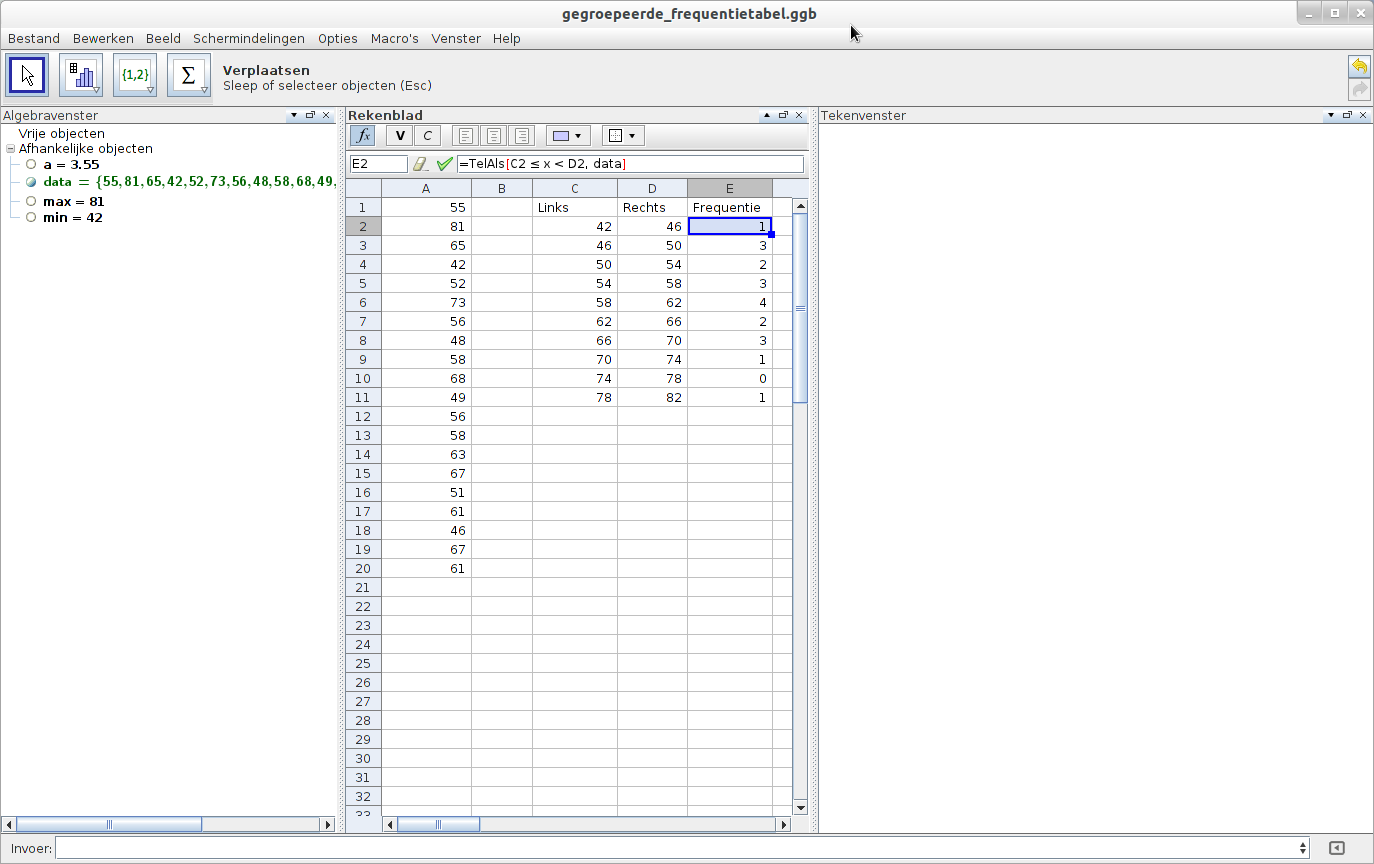
\includegraphics[width=14cm]{gg-gegroepeerde_frequentietabel}
\end{center}




\end{document}


  \item {\bf Absolute cumulatieve frequentie} $cF_j$: Aantal waarnemingen die kleiner dan of gelijk zijn aan deze waarneming.\\
  Berekening: $$cF_j = \sum_{i=1}^jF_i$$
  \item {\bf Relatieve cumulatieve frequentie} $cF_j$: Aantal waarnemingen die kleiner dan of gelijk zijn aan deze waarneming.\\
  Berekening: $$cF_j = \sum_{i=1}^jF_i$$
















\section{Iets statistisch onderzoeken}

We wensen een statistisch onderzoek uit te voeren. Wat wil dit zeggen? Wel, {\it onderzoeken} is iets nauwkeurig nazien of nagaan. Een voorbeeld zou kunnen zijn: {\it Tot hoe laat mogen jongeren in het weekend uitgaan?}. De vraag die bij een onderzoek hoort noemen we de {\bf onderzoeksvraag}. Een {\it statistisch onderzoek} is dan een onderzoek die verloopt volgens de statistiek. De {\bf statistiek} is de wetenschap van het waarnemen van verschijnselen en het weergeven van de uitkomsten in getallen en figuren. In het vorig voorbeeld wil dit zeggen dat we {\it waarnemen} bij andere jongeren tot hoe laat deze uitgaan. Deze waarnemingen gaan we dan zo goed mogelijk {\it weergeven}, dit met getallen of figuren.

Een onderzoek kan in vier stappen verlopen:
\begin{enumerate}
  \item Wat wil je weten? Hoe ga je meten?
  \item Op speurtocht gaan in de dataset.
  \item Wat heb je gevonden? Hoe ver kan je gaan in je conclusie?
  \item Kernachtig samenvatten van onderzoek.
\end{enumerate}

Wat de stappen inhouden zullen we zien aan de hand van een aantal voorbeelden.

\section{Statistisch onderzoek naar de kleuren van M\&M-snoepjes}

\subsection{De onderzoeksvraag}

\begin{wrapfigure}{r}{0.4\textwidth}
  
\includegraphics[width=0.4\textwidth]{MenM-verpakking.png}
\end{wrapfigure}

Iedereen kent wel M\&M’s, de chocoladesnoepjes met de felgekleurde suikerjasjes. De fabrikant van
M\&M’s stopt verschillende kleuren snoepjes in één verpakking.

Heb je enig idee welke kleuren allemaal voorkomen bij M\&M’s?
Komt elke kleur evenveel voor? Dat ga je nu onderzoeken.

Je hebt hier al een eerste probleem. Wat wil je eigenlijk
onderzoeken? Wil je iets zeggen over de kleuren in je eigen zakje
M\&M”s of wil je iets zeggen over de kleuren van alle M\&M-
snoepjes die door de fabrikant gemaakt worden? Dat zijn nogal
verschillende vragen!

\subsection{Wat wil je weten? Hoe ga je meten?}

\subsubsection{Een dataset maken}

Om goed het onderscheid te maken tussen “alle M\&M’s” en “de snoepjes in jouw zakje M\&M’s”
gebruikt de statistiek twee verschillende woorden. Je spreekt over {\bf populatie} als je “de totale
verzameling” bedoelt (dus alle M\&M-snoepjes in de wereld!). Meestal heb je geen tijd of geld om een volledige
populatie te onderzoeken en daarom bekijk je enkel een klein deeltje van die populatie. Zo’n deeltje
van een populatie wordt in de statistiek een {\bf steekproef} genoemd. De snoepjes die in je zakje
M\&M’s zitten, zijn een heel klein deeltje van alle M\&M’s. Jouw snoepjes zijn dus een steekproef uit
de totale populatie van alle M\&M’s.

Je steekproef bestaat uit dingen die je zelf hebt verzameld, die je dus zelf kan zien en beschrijven
(met getallen en grafieken). Hoe je dat doet, dat ga je in dit onderzoek leren. Maar misschien wil je
daarna ook iets zeggen over alle M\&M’s. Misschien zijn de blauwe snoepjes in jouw zakje in de
meerderheid. Zou je dan kunnen zeggen dat bij alle M\&M’s de blauwe snoepjes het meest
voorkomen? (Let op! Misschien heeft een andere leerling meer rode snoepjes).

Iets zeggen over de totale populatie als je enkel de steekproef ziet, dat is helemaal niet eenvoudig.
Statistiek kan je hierbij helpen. Een eerste hulp die de statistiek je biedt, gaat over de manier waarop
je een steekproef moet trekken. De raadgeving die je hier krijgt, had je waarschijnlijk nooit
verwacht. Om een goede steekproef te trekken, moet je je laten leiden door ... het toeval!

Je laten leiden door het toeval, dat is gemakkelijker gezegd dan gedaan. M\&M's worden gemaakt in verschillende
kleuren volgens een verhouding die door de fabrikant is vastgelegd. Die snoepjes komen terecht in
een reuzegrote container waar ze grondig door elkaar worden gemengd. Daarna wordt uit die
container lukraak een schep snoepjes genomen en die snoepjes worden in een zakje verpakt. Dat
gebeurt natuurlijk allemaal volautomatisch en in superhygiënische omstandigheden.

Die enorme container, waarin miljoenen M\&M’s zitten, kan je beschouwen als een goed model voor
de hele populatie. Een goede steekproef trek je dan als volgt: “goed mengen en dan lukraak trekken”.
Deze manier van werken krijgt in de statistiek de naam “{\bf aselecte steekproef}”. {\bf Aselect} betekent dat elk element van de populatie dezelfde kans heeft om opgenomen te worden tot de steekproef. We eisen ook dat een steekproef {\bf representatief} moet zijn, hiermee bedoelen we dat de steekproef een correct beeld moet geven van de verscheidenheid binnen de populatie. Het
aantal elementen in je steekproef (het aantal getrokken snoepjes) noteer je door de letter “$n$” (dat
noem je de {\bf steekproefgrootte}).

De informatie in je steekproef ga je nu op een overzichtelijke manier opschrijven in een tabel. Zo krijg je de
{\bf gegevensverzameling of dataset}. In zulk een tabel staan op de rijen de {\bf elementen}, deze zijn de objecten die in een statistische studie worden onderzocht. In ons geval heb je voor elke M\&M één rij. In de kolommen staan de {\bf veranderlijken}\footnote{In de context van statistiek mogen we ook {\bf variable} gebruiken in plaats van {\bf veranderlijke}, we zullen beide benamingen dan ook door elkaar gebruiken.}, elke veranderlijke is één welbepaalde eigenschap die je opmeet. Zo kunnen we voor elke M\&M de kleur noteren.



\begin{mmopdracht}
Maak een tabel, de {\bf dataset} waarin je de gegevens zal opschrijven. Als je afkortingen gebruikt, schrijf dan ook op wat die afkortingen betekenen.
\ruitjes{11cm}
\end{mmopdracht}

\begin{oefening}
Noteer bij elke onderzoeksvraag de {\bf elementen} en de {\bf veranderlijke}:
\begin{enumerate}[(a)]
  \item Met welk vervoersmiddel komen de leerlingen naar onze school?
  \arules{2}
  \item Welke is het meest geliefde vak van alle laatstejaars leerlingen in Vlaanderen?
  \arules{2}
  \item Hoeveel computers zijn er per leerling beschikbaar voor gans Avelgem?
  \arules{2}
\end{enumerate}
\end{oefening}

\subsubsection{De dataset: getallen en context}
Bij de dataset die je pas hebt opgesteld is er één kolom waarin je de kleur van de snoepjes hebt
geschreven. Je hebt hier te maken met een “eigenschap van snoepjes”, namelijk “hun kleur”. Dit is
een “veranderlijke” die jij hebt opgemeten. Deze veranderlijke heeft hier de waarden: rood, groen,
blauw, bruin, en geel.
Op kleuren kan je geen zinvolle wiskundige bewerkingen uitvoeren zoals optellen of
vermenigvuldigen. Daarom noemt men de veranderlijke “kleur” een {\bf kwalitatieve veranderlijke}.

Later zullen we een onderzoek zien waarbij de veranderlijke een eigenschap is waarmee wel kan worden gerekend. Een voorbeeld zou zijn: {\em Hoeveel huisdieren heeft een Belgisch gezin?}. Je krijgt dan telkens een aantal. Veranderlijken waarmee gerekend kan worden noemen we {\bf kwantitatieve veranderlijken}.

Er is een belangrijk onderscheid tussen de naam van een veranderlijke en de
verschillende waarden van die veranderlijke.
In dit geval is “kleur” de {\bf naam} van de veranderlijke en “rood, groen, blauw,
...” zijn de mogelijke {\bf waarden}.

\begin{oefening}
Geef bij de volgende veranderlijken aan of het kwalitatieve of kwantitatieve veranderlijken zijn. Geef ook telkens één voorbeeld van een aantal mogelijke waarden.
\begin{center}
\begin{tabular}{p{6cm}|p{3cm}|p{3cm}}
Veranderlijke & Soort & Waarden\\
\hline
De smaak van fruitsnoepjes. & & \\
Het aantal tv-toestellen dat Vlaamse gezinnen bezitten. & &\\
De mate van tevredenheid bij klanten van een supermarkt. & &\\
De afstand die leerlingen moeten afleggen als ze naar school komen. & &\\  
\end{tabular}
\end{center}
\end{oefening}

\subsection{Op speurtocht in de dataset}

Je dataset is de basis voor al je verder onderzoek. De dataset, samen met de beschrijving van hoe je
hem hebt opgemeten, moet je nauwkeurig bewaren.

\subsubsection{Een frequentietabel opstellen}

\begin{mmopdracht}
Gebruik je dataset om een frequentietabel op te stellen. Doe dat zoals hieronder aangegeven.
\end{mmopdracht}

In de eerste kolom schrijf je de kleuren en in de tweede kolom schrijf je hoeveel snoepjes er van die
kleur zijn. Dit aantal heet de {\bf frequentie} van die kleur. Een tabel die je op deze manier opstelt, heet
een {\bf frequentietabel}. Zorg ervoor dat je elke kolom een juiste naam geeft: deze naam schrijf je
bovenaan de kolom.

\begin{center}
  \begin{tabular}{p{4cm}|p{2cm}|p{2cm}}
    Kleur&Frequentie&Rel. Freq.\\
    \hline
    &&\\
    \hline
    &&\\
    \hline
    &&\\
    \hline
    &&\\
    \hline
    &&\\
    \hline
    &&\\
    \hline
    &&\\
    \hline
    &&\\
  \end{tabular}
\end{center}
\vspace{1cm}

\begin{mmopdracht}
Bereken de steekproefgrootte met behulp van de frequentietabel.
\end{mmopdracht}

Hoe heb je dit gedaan?
\arules{3}

We gaan nu een derde kolom aan de frequentietabel toevoegen. In die kolom komt, per kleur, {\bf de
relatieve frequentie}. De relatieve frequentie is niets anders dan de frequentie gedeeld door het totale
aantal $n$ (de steekproefgrootte) . Je kan dit getal ook in percent uitdrukken. Als je voor “geel” een relatieve frequentie van
0.16 vindt, dan kan je dat ook schrijven als 16\%. Hierbij rond je af op één eenheid. In woorden zeg
je dat 16\% van jouw onderzochte snoepjes geel is. De relatieve frequentie maakt het mogelijk om kansen
te schatten die theoretisch moeilijker te bepalen zijn.

\newpage
\begin{mmopdracht}
Bepaal de relatieve frequentie voor de frequentietabel, vul daarvoor de kolom {\bf Rel. Freq.} aan.
\end{mmopdracht}

Hoe heb je dit gedaan?
\arules{3}


\begin{mmopdracht}
Als er in de volledige populatie, dus alle snoepjes in het vat, 6 kleuren zitten. En
van elk kleur zijn er evenveel snoepjes. Wat is dan de kans om lukraak een geel snoepje te kiezen?
\arules{3}
\end{mmopdracht}

\begin{mmopdracht}
De relatieve frequentie voor {\em geel} wijkt af van de theoretische kans, verklaar dit en wanneer
zou de relatieve frequentie dichter bij de theoretische kans moeten komen?
\arules{3}
\end{mmopdracht}

Waar mogelijk zullen we de berekeningen ook met de computer doen. Er zijn verschillende computer programma's die ons kunnen helpen met een statistisch onderzoek. Wij zullen steeds {\it Geogebra}\footnote{\url{http://www.geogebra.org/}} gebruiken.

We starten {\it Geogebra}. Toon het algebravenster en het rekenblad. Het tekenblad mag verborgen worden. Je selecteert hiervoor:
\begin{itemize}
  \item \menulist{Beeld:Algebravenster} Aan,
  \item \menulist{Beeld:Rekenblad} Aan,
  \item \menulist{Beeld:Tekenblad} Uit.
\end{itemize}
Het rekenblad is onze rekenruimte. Deze bevat allemaal verschillende {\bf cellen}. Deze cellen hebben een naam. De cel linksboven noemt \verb#A1#. De \verb#A# staat voor de eerste kolom. {\bf Kolommen} verdelen het rekenblad verticaal. De \verb#1# staat voor de eerste rij. {\bf Rijen} verdelen het rekenblad horizontaal.

De eerste kolom vullen we met de frequenties. Als je bijvoorbeeld $13$ rode, $9$ groene, $8$ gele, $7$ oranje, $7$ bruine en $6$ blauwe snoepjes had, dan ga je als volgt te werk:
\begin{itemize}
  \item In cell \verb#A1# vul je het getal $13$ in.
  \item In cell \verb#A2# vul je het getal $9$ in.
  \item \ldots
  \item In cell \verb#A6# vul je het getal $6$ in.
\end{itemize}
De cellen \verb#A1# tot \verb#A6# kunnen we kort noteren als \verb#A1:A6# en noemen we een {\bf lijst}.

In de tweede kolom, zal je Geogebra de relatieve frequentie laten bereken. De relatieve frequentie is de frequentie gedeeld door de steekproefgrootte. We hebben dus eerst nog de steekproefgrootte nodig. We laten Geogebra dit uitrekenen door de som uit te rekenen van de lijst \verb#A1:A6# en deze waarde op te slaan in $n$:
\begin{itemize}
  \item Voer in het invoerveld het commando \verb#n=Som[A1:A6]# in.
\end{itemize}

In het rekenblad zal nu $n=50$ verschijnen. Vanaf nu weet Geogebra dat de steekproefgrootte $n=50$ is. Nu selecteer je de eerste cel in de tweede kolom en laat bereken je de relatieve frequentie. Je doet dit door aan Geogebra te laten weten dat eerst iets moet worden berekend, dit kan je door te beginnen met een is gelijk aan teken (\verb#=#). Geogebra moet de frequentie \verb#A1# dan delen door de steekproefgrootte \verb#n#:
\begin{itemize}
  \item In cell \verb#B1# vul je \verb#=A1/n# in en druk op enter.
\end{itemize}

Dezelfde berekening moet nu worden uitgevoerd voor de andere cellen in de tweede kolom. In plaats van zelf opnieuw alle waarden in te vullen kan je Geogebra dit zelf laten doen. Hiervoor moet je de berekening uit de eerste cel {\emph slepen} naar de cellen eronder:
\begin{itemize}
  \item Selecteer cel \verb#B1#
  \item Click op het vierkantje rechtsonder in de cel, en blijf de muisknop ingedrukt houden terwijl je naar beneden sleept.
  \item Laat de muisknop pas los in de cel \verb#B6#.
\end{itemize}

\begin{center}
  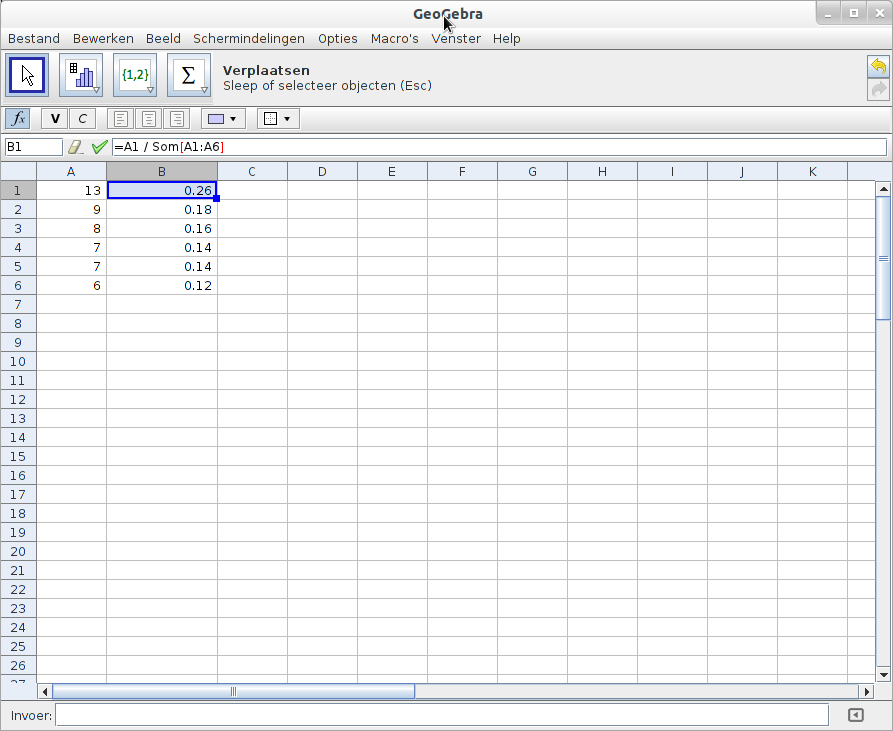
\includegraphics[width=14cm]{gg-relatieve_frequentie.png}
\end{center}

\begin{mmopdracht}
Voeg aan je tabel een derde kolom toe met naam “relatieve frequentie” en schrijf daarin de
resultaten die in Geogebra staan (in percent). Tel de percenten bij elkaar op. Hoeveel heb je?
\arules{1}
\end{mmopdracht}

Soms heb je frequenties nodig, in andere gevallen gebruik je relatieve frequenties. Als je aantallen
bestudeert, dan werk je met frequenties. Als je percentages gebruikt om twee onderzoeken met
elkaar te vergelijken, dan werk je met relatieve frequenties.

{\bf Voorbeeld}\\
Om te weten of je genoeg rode snoepjes hebt om er eentje te kunnen geven aan elk van je 10
vrienden, dan kijk je naar de frequentie.
Als je de kleurensamenstelling van een grote en een kleine zak M\&M’s wil vergelijken, dan zal je
met percentages werken en dus relatieve frequenties gebruiken.

\begin{oefening}
Noteer van de volgende onderzoeken telkens de populatie, de steekproef en de steekproefgrootte.
\begin{enumerate}[(a)]
  \item Een interviewer vraagt telefonisch aan 500 Vlamingen of ze voor of tegen nieuwe verkiezingen zijn.
  \begin{itemize}
    \itemsep0.5em
    \item Populatie: \arulefill
    \item Steekproef: \arulefill
    \item Steekproefgrootte: \arulefill
  \end{itemize}
  \item Na elke rit in de Ronde van Frankrijk wordt een aantal renners onderzocht op doping.
  \begin{itemize}
    \itemsep0.5em
    \item Populatie: \arulefill
    \item Steekproef: \arulefill
    \item Steekproefgrootte: \arulefill
  \end{itemize}
\end{enumerate}
\end{oefening}

\begin{oefening}
In september werd aan alle leerlingen van het derde jaar gevraagd of ze een rekentoestel hadden, en zo ja, van welk merk. Vervolledig de frequentietabel.
\begin{center}
\begin{tabular}{l|c|c}
Rekenmachine & Frequentie & Rel. Freq\\\hline
Geen & & 0.54\\\hline
Casio & 27 & 0.18\\\hline
TI & &\\\hline
n= & &\\
\end{tabular}
\end{center}
\end{oefening}

\subsubsection{Figuren tekenen}

\begin{wrapfigure}{r}{0.3\textwidth}
  \vspace{-0.5cm}
  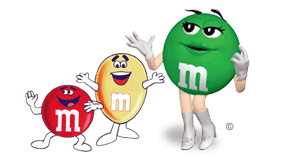
\includegraphics[width=0.3\textwidth]{MenM-fun.png}
\end{wrapfigure}

Veruit het meest belangrijke onderdeel bij de studie van een
dataset is kijken naar figuren. Dit is niet eenvoudig en je
moet stapsgewijs leren waar je allemaal moet op letten.
Zodra je dit wat kent, kan je uit een figuur heel veel
informatie halen. Maar je moet natuurlijk eerst weten welke
figuur je moet maken en hoe je die moet tekenen.

\subsubsection*{Een staafdiagram}

Je hebt in dit onderzoek een kwalitatieve veranderlijke opgemeten. Voor dit soort
veranderlijke is het {\bf staafdiagram} de basisfiguur.

Als voorbeeld zie je hier een staafdiagram
van de Vlaamse bevolking per provincie. De
informatie die hier wordt weergegeven, kan
je vinden in het boekje “Vlaanderen in
cijfers” op de website:
\url{http://www4.vlaanderen.be/dar/svr/Cijfers/Pages/Excel.aspx}.

  
\begin{minipage}{0.5\textwidth}
De namen van de provincies zijn afgekort als:
  \begin{description}
    \item[Antw] Antwerpen,
    \item[O-Vl] Oost-Vlaanderen,
    \item[W-Vl] West-Vlaanderen,
    \item[Vl-Br] Vlaams - Brabant,
    \item[Limb] Limburg.
  \end{description}
\end{minipage}
\begin{minipage}{0.5\textwidth}
%  \definecolor{qqqqff}{rgb}{0,0,1}
\begin{tikzpicture}[scale=0.1,line cap=round,line join=round,>=triangle 45,x=1.0cm,y=1.0cm]
\draw[-,color=black] (-9.63,0) -- (78.66,0);
\draw[color=black] (60,0.13) node [anchor=south west] { Provincie};
\draw[-,color=black] (0,-4.46) -- (0,27.9);
\draw[color=black] (0.57,27.25) node [anchor=west] { Aantal inwoners};
\clip(-9.63,-4.46) rectangle (78.66,27.9);
\draw[fill=black,fill opacity=0.1] (7,0) rectangle (12.5,8.39);
\draw[fill=black,fill opacity=0.1] (12.5,0) rectangle (17.5,0);
\draw[fill=black,fill opacity=0.1] (17.5,0) rectangle (22.5,10.77);
\draw[fill=black,fill opacity=0.1] (22.5,0) rectangle (27.5,0);
\draw[fill=black,fill opacity=0.1] (27.5,0) rectangle (32.5,11.59);
\draw[fill=black,fill opacity=0.1] (32.5,0) rectangle (37.5,0);
\draw[fill=black,fill opacity=0.1] (37.5,0) rectangle (42.5,14.32);
\draw[fill=black,fill opacity=0.1] (42.5,0) rectangle (47.5,0);
\draw[fill=black,fill opacity=0.1] (47.5,0) rectangle (52.5,17.45);
\draw (48.1,-0.39) node[anchor=north west] {Antw};
\draw (18.33,-0.43) node[anchor=north west] {Vl-Br};
\draw (28.4,-0.43) node[anchor=north west] {W-Vl};
\draw (38.13,-0.43) node[anchor=north west] {O-Vl};
\draw (7.91,-0.36) node[anchor=north west] {Limb};
\draw (46.85,24) node[anchor=north west] {1744862};
\draw (16.74,18) node[anchor=north west] {1076924};
\draw (26.93,12.35) node[anchor=north west] {1159366};
\draw (36.66,15.08) node[anchor=north west] {1432326};
\draw (7.23,9.13) node[anchor=north west] {838505};
\begin{scriptsize}
\fill [color=qqqqff] (0,0) circle (1.5pt);
\end{scriptsize}
\end{tikzpicture}

  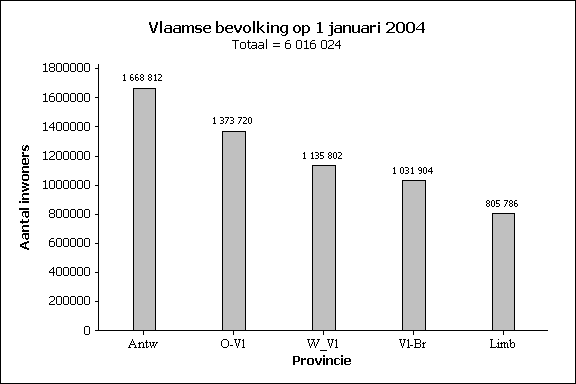
\includegraphics[width=8cm]{vlaamse_bevolking.png}
\end{minipage}

Om een staafdiagram te tekenen op basis van jouw frequentietabel ga je als volgt te werk:
\begin{enumerate}
  \item Op de $x$-as zet je de verschillende kleuren. Hoewel de waarden van de kwalitatieve variabele, kleur, geen natuurlijke volgorde hebben, zal je toch moeten kiezen hoe je de kleuren ordent op de $x$-as. Welke kleur komt als eerste? Welke kleur komt als tweede? Waarom maak je die keuze?

De kleuren van een snoepje hebben geen natuurlijke volgorde. We rangschikken daarom de
bijhorende frequenties. Dat zijn getallen en die hebben wel een natuurlijke volgorde. Je kan
bijvoorbeeld rangschikken van groot naar klein. Voor kleuren met gelijke frequenties kan je
de onderlinge plaats zelf kiezen.
\item Op de $y$-as duid je de frequentie van elke kleur aan en je tekent dan bij elke kleur een staafje
waarvan de lengte overeenkomt met de frequentie van die kleur. Zorg ervoor dat alle staafjes
los van elkaar staan.
\item Voorzie de assen van de juiste naam.
\end{enumerate}

\begin{mmopdracht}
Teken nu zo’n staafdiagram voor het onderzoek.
\begin{center}
\begin{tikzpicture}[line cap=round,line join=round,>=triangle 45,x=1.0cm,y=1.0cm]

\draw [gray, very thin, step=0.5cm] (0,0) grid (15,10);
\draw[-,black,very thick] (0,2) -- (15,2);
\draw[-,black,very thick] (2,0) -- (2,10);
\end{tikzpicture}
\end{center}
\end{mmopdracht}

Zulk staafdiagram kan ook met Geogebra gemaakt worden:
\begin{itemize}
  \item Vul een rekenblad in met de frequenties, zorg dat de frequenties in de cellen van \verb#B2# tot \verb#B7# terechtkomen.
  \item Maak vanuit het rekenblad een lijst aan van de frequenties aan door:
  \begin{itemize}
    \item de cellen \verb#B2:B7# te selecteren,
    \item rechts te klikken op de geselecteerde cellen,
    \item het menu \menulist{Creëer:Lijst} te selecteren,
    \item de aangemaakte lijst "Lijst1" te hernoemen naar "frequenties" door:
    \begin{itemize}
      \item in het algebravenster recht te clicken op de nieuwe lijst, lijst1,
      \item het menu \menulist{Naam wijzigen} te selecteren,
      \item "frequenties" te typen in het dialoogvenster
    \end{itemize}
  \end{itemize}
  \item Maak ook een lijst met posities aan. Typ hiervoor in het invoervenster\\
  \verb$posities={10,20,30,40,50,60}$.
  \item Teken nu het staafdiagram met het commando \verb$Staafdiagram[posities,frequenties,5]$
  \item Wijzig nu de schaal van de assen door deze te verslepen.
  \item Voeg nu tekst in om alle labels aan te vullen.
\end{itemize}

\begin{center}
  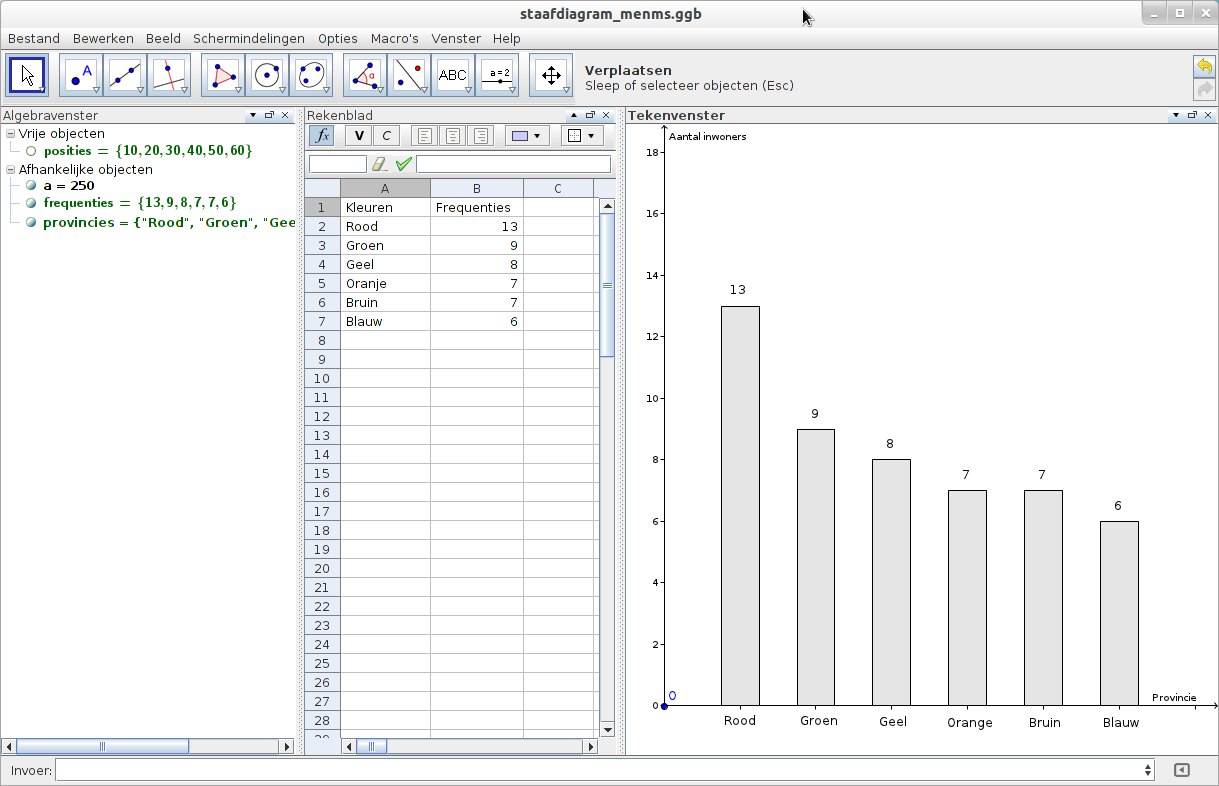
\includegraphics[width=14cm]{gg-staafdiagram_menms}
\end{center}

\subsubsection*{Een taartdiagram}
Misschien wil je de relatieve frequenties van de kleuren grafisch voorstellen. Dan kan je opnieuw een
staafdiagram tekenen, waarbij je in de $y$-richting staafjes tekent waarvan de lengte gelijk is aan de
relatieve frequentie.
Maar er is ook een andere figuur die de relatieve frequentie (meestal uitgedrukt in percent) mooi
weergeeft. Dat is het {\bf taartdiagram of cirkeldiagram}.

Bij het tekenen van een taartdiagram verdeel je een cirkeloppervlak in stukken, juist zoals je een
taart in stukken snijdt. Eén zo'n stuk heet een {\bf sector}. De totale oppervlakte van de cirkel komt overeen
met de som van alle percentages en dat is 100\%.

Voor een taartdiagram maken we enkele afspraken:
\begin{itemize}
  \item Begin bovenaan en draai met de wijzers van de klok mee.
  \item De grootste sector komt eerst, dan komt de tweede
grootste, enzovoort.
\end{itemize}

\newpage
\begin{wrapfigure}[11]{r}{0.3\textwidth}
  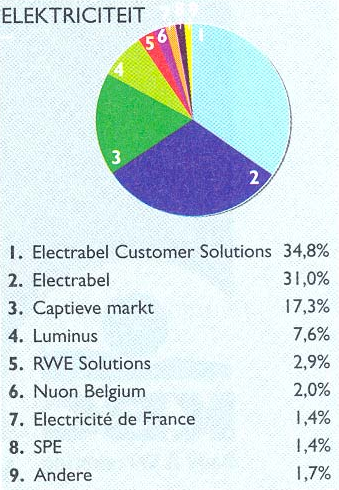
\includegraphics[width=0.3\textwidth]{cirkeldiagram_electriciteit}
\end{wrapfigure}
Je ziet hier een voorbeeld van de marktaandelen van
energiebevoorraders in België. Het gaat over de elektriciteit in
het jaar 2004. Deze figuur staat in het weekblad Knack van 22
juni 2005 en is goed leesbaar. Maar als je een krant of
weekblad doorbladert, dan zie je soms verwarrende en zelfs
verkeerde grafieken.

Hoeveel graden elke sector is, bereken je door de relatieve
frequentie te vermenigvuldigen met $360\degree$. Dit doe je met je
rekenmachine. Maak daarna “verstandige” afrondingen zodat
alle sectoren samen terug $360\degree$ geven (je kan
eventueel enkele keren tot op een halve graad werken).

Om een taartdiagram te tekenen op basis van jouw onderzoek begin je als volgt.

\begin{mmopdracht}
Bereken eerst voor elke relatieve frequentie hoe groot de sector is die daarbij hoort. Gebruik
je rekenmachine.
\begin{center}
  \begin{tabular}{|p{1.5cm}|p{1.5cm}|p{1.5cm}|p{1.5cm}|p{1.5cm}|p{1.5cm}|p{1.5cm}|}
    \hline
    kleur:\vspace{0.5cm}&&&&&&\\
    \hline
    hoek:\vspace{0.5cm}&&&&&&\\
    \hline
  \end{tabular}
\end{center}
\end{mmopdracht}

\begin{mmopdracht}
Teken nu cirkelsectoren die overeenstemmen met de relatieve frequenties. Schrijf bij elke
sector met welke kleur van snoepje hij overeenkomt en noteer ook de relatieve frequentie in
percentvorm erbij. Je kan natuurlijk ook de sector inkleuren met de bijhorende kleur.
\begin{center}
\begin{tikzpicture}[scale=0.75,line cap=round,line join=round,>=triangle 45,x=1.0cm,y=1.0cm]
\draw(5,5) circle (5cm);
\draw (5,5)-- (5,10);
\end{tikzpicture}
\end{center}
\end{mmopdracht}

Ook met Geogebra kunnen we een cirkeldiagram maken. We vertrekken vanuit het zelfde bestand als bij
het staafdiagram. De frequentie moeten we nu omzetten naar het aantal graden dat het sector is. Maak
hiervoor eerst het totaal van alle frequenties, met andere woorden de steekproefgrootte $n$.
\begin{itemize}
  \item Vul in het algebra venster \verb$n=Som[B2:B7]$ in.
\end{itemize}
Vul nu in de cellen naast de frequentie de relatieve frequentie in volgens een cirkel. Je moet daarvoor de frequentie delen door de steekproefgrootte, en dan vermenigvuldigen met het aantal graden die een cirkel bevat:
\begin{itemize}
  \item Vul in de cel \verb#C2# de formule \verb#=B2 / n * 360#$\degree$ in.
  \item Selecteer nu opnieuw de cel \verb#C2# en sleep deze naar onder.
\end{itemize}

Nu we de graden hebben berekend voor de sectoren van het cirkeldiagram maken we de figuur. Creëer eerst twee punten. $A$ op $(0,0)$ en $B$ op $(0,5)$. Creëer nu een cirkel met als middelpunt $A$ en als straal $B$. Klik nu op het icoontje {\it Hoek met gegeven grootte}. Klik eerst op $B$ en dan op $A$ en als hoekgrootte geef je \verb$C2$ in. Klik nu op het icoontje {\it Cirkelsector met middelpunt door 2 punten}. Als eerste punt geef je $A$, als tweede punt geef je $B'$ en uiteindelijk als derde punt geef je $B$. Herhaal dit nu voor de andere sectoren.

De figuur kan afgewerkt worden door tekst in te voeren en de kleuren van de sectoren te wijzigen:
\begin{center}
  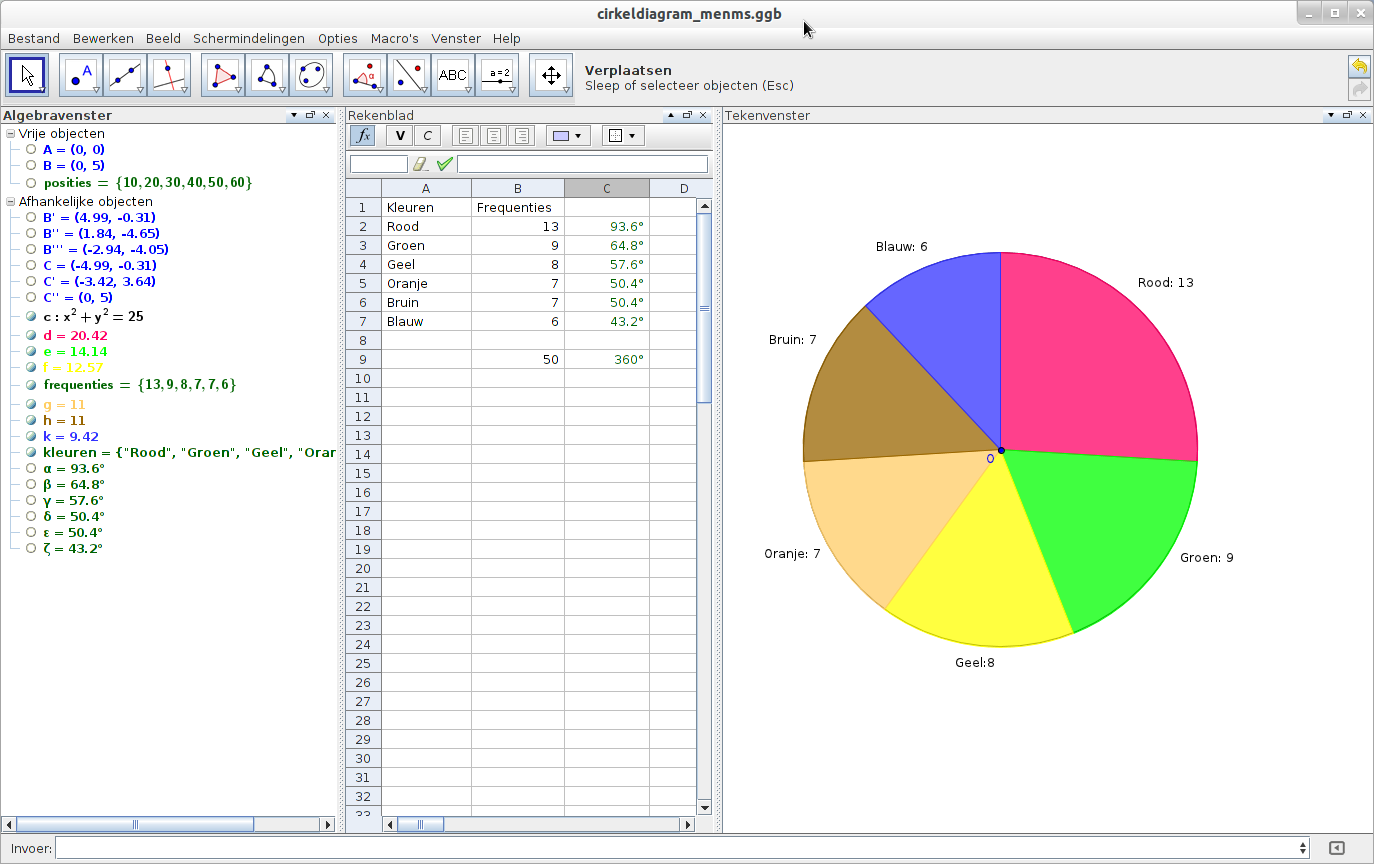
\includegraphics[width=14cm]{gg-cirkeldiagram_menms}
\end{center}

\subsection{Wat heb je gevonden? Hoever kan je gaan in je conclusie?}

\subsubsection{De variabiliteit van steekproefresultaten}

Je hebt nu de kleur van de snoepjes in een zakje M\&M’s bestudeerd met behulp van een
frequentietabel, een staafdiagram en een taartdiagram. Laten we nu eens kijken naar de
inhoud van een aantal andere zakjes M\&M's.

\begin{mmopdracht}
Verwacht je dat de andere zakjes dezelfde resultaten zullen hebben als het eerste zakje?
\arules{7}
\end{mmopdracht}

\begin{mmopdracht}
Kan je je antwoord op vorige vraag wat verduidelijken door te verwijzen naar de manier
waarop die zakjes gevuld worden? Kan je hierbij ook de woorden populatie en steekproef op
een juiste wijze gebruiken?
\arules{4}
\end{mmopdracht}

In plaats van naar alle kleuren te kijken, zou je er eens je lievelingskleur kunnen uithalen,
bijvoorbeeld blauw. Hoeveel percent blauwe snoepjes zaten er in het eerste zakje? En hoeveel percent
blauwe snoepjes waren er in de andere zakjes?

\begin{mmopdracht}
Noteer voor elk onderzocht zakje telkens het percent blauwe snoepjes.
\arules{5}
\end{mmopdracht}

\begin{mmopdracht}
Als jij maar één zakje snoepjes mag onderzoeken (bijvoorbeeld het eerste) en je zou moeten raden hoeveel percent blauwe snoepjes er door de fabrikant gemaakt wordt (dus hoeveel percent blauwe
snoepjes er in de totale populatie zit), wat zou jij dan antwoorden?
\arules{1}
\end{mmopdracht}

\begin{mmopdracht}
Is je bovenstaand antwoord exact juist? Hoe weet je dat?
\arules{5}
\end{mmopdracht}

\subsubsection{Steekproefgrootte, nauwkeurigheid en haalbaarheid}

Met het onderzoek van de snoepjes in een aantal zakjes M\&M’s wil je een zicht krijgen op alle
M\&M-snoepjes. Je zou bijvoorbeeld willen weten hoeveel percent van alle M\&M’s blauw zijn of op
welke manier de kleuren verdeeld zijn.

Een eerste (maar naïeve) reactie zou kunnen zijn: wel, onderzoek dan de totale populatie. Maar dat
voorstel is helemaal niet haalbaar! Je gaat toch niet alle zakjes openmaken om te kijken wat de kleur
van de snoepjes is. Dat zou niet alleen veel te veel tijd en geld vragen, het is gewoon onmogelijk
omdat de snoepjes dan niet meer kunnen verkocht worden. Daarom onderzoek je dus maar een
beperkt aantal snoepjes: je verzamelt informatie over een deel van de M\&M’s om zo conclusies te
trekken over alle M\&M’s.

Herinner je de twee belangrijke begrippen:
\begin{itemize}
  \item De hele groep objecten (of personen) waarover je iets wil weten, heet de {\bf populatie}.
  \item Een {\bf steekproef} is een deel uit deze populatie.
\end{itemize}

Als het praktisch haalbaar is en als je op een goede manier steekproeven trekt, dan is het beter om
met een grotere steekproef te werken dan met een kleinere. Intuïtief kan je dit waarschijnlijk wel
begrijpen. Als je een groter aantal M\&M’s uit de totale populatie mag trekken, dan heb je meer
informatie. Maar ook een grote steekproef is nog altijd aan het toeval onderhevig. Als je echter
meerdere keren een grote steekproef zou trekken, dan zou je zien dat op grotere steekproeven minder
schommelingen zitten dan op kleinere.

Om een grotere steekproef te krijgen brengen we nu alle open gedane zakjes M\&M's samen en gebruiken
we deze als één grote steekproef.

\begin{mmopdracht}
De verschillende resultaten van elk onderzocht zakje worden nu verzameld. Noteer alle
cijfers die op bord komen en maak dan een nieuwe frequentietabel met daarin per kleur de
frequentie en de relatieve frequentie voor de snoepjes van de totale klas.
\begin{center}
  \begin{tabular}{p{2cm}|p{1cm}|p{1cm}|p{1cm}|p{1.5cm}|p{1.5cm}}
    Kleur&Freq. $Z_1$ & Freq. $Z_2$ & Freq. $Z_3$ & Freq. &Rel. Freq.\\
    \hline
    &&&&\\
    \hline
    &&&&\\
    \hline
    &&&&\\
    \hline
    &&&&\\
    \hline
    &&&&\\
    \hline
    &&&&\\
    \hline
    &&&&\\
    \hline
    &&&&\\
  \end{tabular}
\end{center}
\end{mmopdracht}

\subsubsection{Een model voor de populatie}

\begin{wrapfigure}[7]{l}{0.3\textwidth}
  \vspace{-0.5cm}
  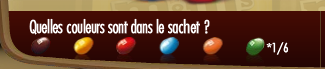
\includegraphics[width=0.3\textwidth]{MenM-uniforme_verdeling}
  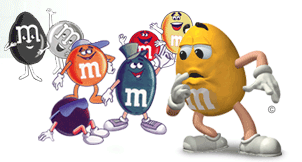
\includegraphics[width=0.3\textwidth]{MenM-hoeveel}
\end{wrapfigure}
Hoe de echte populatie van alle M\&M-snoepjes eruitziet, zal niemand ooit weten. Je kan toch niet
naast die productielijn gaan staan en voor die miljoenen (miljarden?) snoepjes de kleur noteren.
Maar een model voor de populatie bestaat wel. In België worden geen M\&M’s gemaakt. Zij worden
ingevoerd uit naburige landen. Bij M\&M’s uit Frankrijk komen alle kleuren globaal (in de populatie)
evenveel voor.

Als je nu mag aannemen dat (volgens de fabrikant) alle
kleuren evenveel voorkomen dan kan je deze eigenschap
gebruiken om een model te maken voor de totale
populatie. Aan de andere kant heb jij nu cijfers van een
grote steekproef uit die populatie. Het is dus interessant
om het model voor de populatie te vergelijken met wat je
ziet in die grote steekproef. Je zou hiervoor twee
afzonderlijke staafdiagrammen kunnen tekenen maar je
kan die vergelijking ook in één en dezelfde figuur
voorstellen.

\begin{mmopdracht}
Maak een tabel waarin je aangeeft hoe de populatie er precies uitziet. Gebruik je frequenties
of relatieve frequenties in die tabel?
\begin{center}
  \begin{tabular}{p{2cm}|p{2cm}}
    Kleur&Rel. Freq.\\
    \hline
    &\\
    \hline
    &\\
    \hline
    &\\
    \hline
    &\\
    \hline
    &\\
    \hline
    &\\
  \end{tabular}
\end{center}
\end{mmopdracht}

\begin{mmopdracht}
Hoe zou de grafiek er in dit geval uit zien?
\arules{2}
\end{mmopdracht}

\begin{mmopdracht}
Kan je verklaren waarom jouw cijfers eventueel afwijken van die van de fabrikant?
\arules{6}
\end{mmopdracht}

\subsection{Kernachtige samenvatting van dit onderzoek}

Een statistisch onderzoek wordt niet zomaar in het wilde weg gedaan. Meestal is er een
opdrachtgever (bedrijf, overheid, organisatie, ...) die bepaalde informatie nodig heeft. De statisticus
die het onderzoek heeft uitgevoerd zal dan ook zijn onderzoeksresultaten zorgvuldig moeten
presenteren bij die opdrachtgever.

Op dit ogenblik heb je al heel wat informatie over het onderzoek. Deze informatie moet je nu nog
vervolledigen met:
\begin{itemize}
  \item antwoorden op de contextvragen
  \item besluiten over het uitgevoerde onderzoek.
\end{itemize}

De contextvragen of www-vragen, die bij elk onderzoek aan bod komen, zijn:
\begin{enumerate}
  \item {\bf Waarom} is dit onderzoek uitgevoerd? (Wie wilt wat weten?)
  \item {\bf Waar} is dit onderzoek uitgevoerd? (In het buitenland? In mijn gemeente?)
  \item {\bf Wanneer} is dit onderzoek uitgevoerd? (Vorige eeuw? Dit jaar?)
  \item {\bf Wie of wat} wordt onderzocht? (Bij wie worden dingen opgemeten? Wat zijn de
“elementen”?)
  \item {\bf Wat} wordt er juist opgemeten?( Wat wordt er per element allemaal genoteerd? Wat
zijn de “veranderlijken”?)
  \item {\bf Hoe} wordt dit onderzoek uitgevoerd?( Hoe zijn de “elementen” verzameld? Hoe zijn
mensen bij een enquête gecontacteerd?)
\end{enumerate}

\begin{mmopdracht}
Formuleer in een bondige tekst de antwoorden op de contextvragen.
\arules{8}
\end{mmopdracht}

Nu kan je conclusies trekken. Maar je hebt al begrepen dat statistische besluiten rekening moeten
houden met toevallige uitkomsten en dus niet hetzelfde zijn als wiskundige bewijzen.
Wees dus voorzichtig bij je besluit. Als er problemen zijn opgetreden, vermeld die dan. Zo kom je
tot een genuanceerd rapport.

\begin{mmopdracht}
Formuleer in een bondige tekst je besluiten over het uitgevoerde onderzoek.
\arules{8}
\end{mmopdracht}

%\begin{center}
%  
\includegraphics[width=0.3\textwidth]{MenM-snoepjes_banner}
%\end{center}

\subsection{Zelfevaluatie}
In dit onderzoek heb je geleerd over:\\
\begin{wrapfigure}[13]{r}{0.2\textwidth}
  \vspace{1cm}
  
\includegraphics[width=0.2\textwidth]{MenM-zelfeval}
\end{wrapfigure}
\vspace{-1cm}
\begin{itemize}
  \item de context van een statistisch onderzoek (wanneer, waar,...)
  \item het onderscheid tussen de populatie en een steekproef
  \item een aselecte steekproef
  \item de structuur van een dataset (elementen, veranderlijken)
  \item kwalitatieve veranderlijken
  \item de frequentietabel bij een kwalitatieve veranderlijke
  \item het staafdiagram bij een kwalitatieve veranderlijke
  \item het taartdiagram bij een kwalitatieve veranderlijke
\end{itemize}

Je bent nu in staat om de volgende opdrachten uit te voeren:

\begin{oefening}
Zeg in eigen woorden op welke vragen je een antwoord moet kunnen geven als men vraagt
naar de context van een statistisch onderzoek.
\arules{4}
\end{oefening}

\begin{oefening}
Omschrijf de begrippen steekproef en populatie in je eigen woorden en geef een (nieuw)
voorbeeld. Leg voor jouw voorbeeld uit hoe je daar een aselecte steekproef zou
trekken.
\arules{4}
\end{oefening}

\begin{oefening}
Leg duidelijk uit hoe een dataset eruitziet. Gebruik hiervoor een nieuw voorbeeld dat je zelf
hebt bedacht.
\arules{4}
\end{oefening}

\begin{oefening}
Zeg in eigen woorden wanneer je over een kwalitatieve veranderlijke spreekt. Is de bloedgroep zo’n veranderlijke? Kan je zelf een kwalitatieve veranderlijke bedenken?
\arules{4}
\end{oefening}


Als je opmetingen hebt van een kwalitatieve veranderlijke, dan moet je daarvoor
een frequentietabel, een staafdiagram en een taartdiagram kunnen maken.

Soms kom je de uitdrukking “horizontaal staafdiagram” tegen. Kijk daarvoor naar de figuur
die je vindt in de Gazet van Antwerpen van 3 november 2004. Voor de 364 jobs die in
oktober 2004 bij de 4 grootste faillissementen in Vlaanderen verloren gingen, heeft men een
figuur getekend.

\begin{center}
  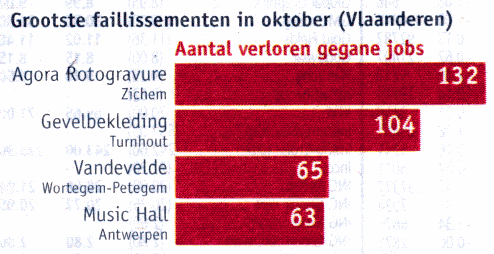
\includegraphics[width=0.6\textwidth]{horizontaal_staafdiagram-faillissementen}
\end{center}


\begin{oefening}
\begin{itemize}
\item Welke veranderlijke is er genoteerd bij elke persoon die zijn job is kwijtgeraakt?
\arules{1}
\item Welk soort veranderlijke is dat?
\arules{1}
\item Wat zijn haar waarden?
\arules{2}
\item Is de figuur goed getekend?
\arules{2}
\end{itemize}
\end{oefening}

\begin{wrapfigure}[7]{r}{0.6\textwidth}
  \vspace*{-1.5cm}
  \centering
  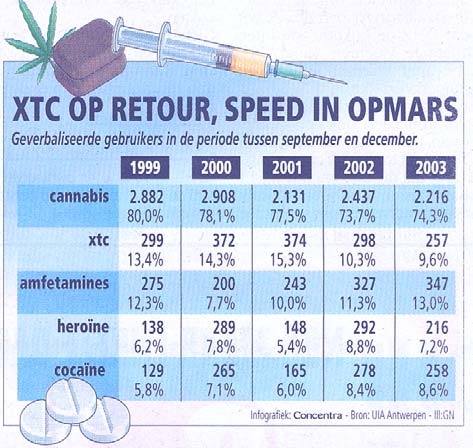
\includegraphics[width=0.5\textwidth]{tabel-drugs}
\end{wrapfigure}
\vspace*{1cm}
Als je een frequentietabel ziet, dan moet je die juist kunnen interpreteren. Bekijk de tabel over XTC en Speed (Gazet van Antwerpen van 20-10-2004). Kijk enkel naar de informatie die daarin staat over het jaar 2003.

\begin{oefening}
\begin{itemize}
  \item Is “druggebruik” daar behandeld als een kwalitatieve veranderlijke?
  \arules{2}
  \item Is de tabel correct?
  \arules{3}
\end{itemize}
\end{oefening}

\begin{oefening}
Een bestaande figuur moet je juist kunnen interpreteren. Bekijk het taartdiagram over de
vrijetijdsbesteding van jongeren (De Standaard van 6-12-2000).

\begin{center}
  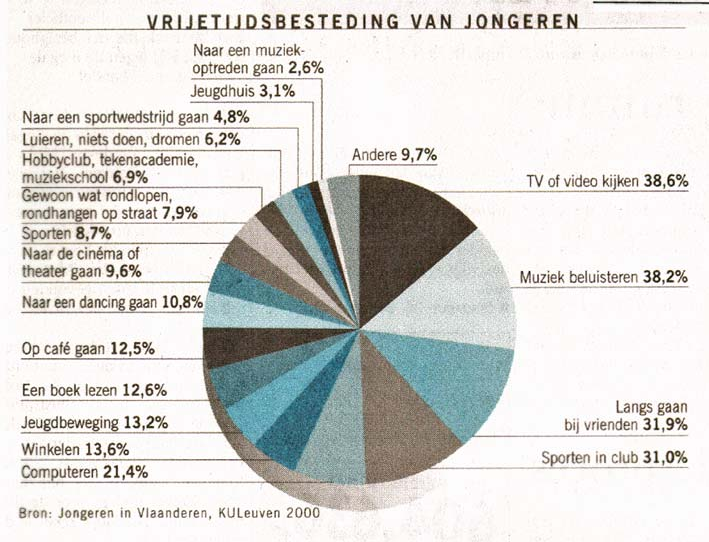
\includegraphics[width=0.7\textwidth]{cirkeldiagram-vrijetijdsbesteding}
\end{center}

\begin{itemize}
  \item Is “vrijetijdsbesteding” hier behandeld als een kwalitatieve veranderlijke?
  \arules{3}
  \item Is het taartdiagram correct getekend?
  \arules{3}
\end{itemize}
\end{oefening}

\section{Een statistisch onderzoek naar het schatten van de tijdsduur van 1 minuut}

\subsection{Wat wil je weten? Hoe ga je meten?}

\subsubsection{De onderzoeksvraag}

In sporten zoals atletiek, zwemmen en Formule 1 speelt tijdsopname een belangrijke rol. Probeer je
eens voor te stellen wat in de cockpit van een Ferrari gebeurt om de rondetijden tot op een duizendste
van een seconde te kunnen opmeten.

De meest primitieve manier van tijdsopname is vermoedelijk gewoonweg ... tellen. Je kent
waarschijnlijk het 21 – 22 – 23 trucje om 3 seconden te benaderen, maar de tijdsduur van één minuut
schatten is heel wat moeilijker. Of niet? Aan jou de uitdaging om dit te onderzoeken!

Let op! Wat is je populatie?\\
Je hebt hier opnieuw een probleem. Je moet eerst heel nauwkeurig zeggen wat je bij welke populatie
wil onderzoeken. Misschien wil je weten hoe één bepaalde leerling een minuut schat, om te
constateren dat zij een kwart van de keren te hoog en drie kwart van de keren te laag schat. Dan
bestaat je populatie (in theorie) uit alle resultaten van die leerling, als je die miljoenen keren een
minuut zou laten schatten. En als steekproef zal je dan die éne leerling 40
keren laten schatten. Zo krijg je een idee over het schattingsgedrag van die
éne leerling.

Maar je kan ook iets anders willen weten. Hoe schatten de leerlingen op je
school, als zij één keer de kans krijgen om te schatten? Je populatie bestaat
dan uit alle leerlingen van je school. Daaruit kan je een steekproef trekken
van 40 leerlingen, die één keer de kans krijgen om een minuut te schatten.
We spreken af dat je dit tweede probleem gaat onderzoeken.

\begin{stopdracht}
Wat onderzoek je hier bij welke populatie?
\arules{4}
\end{stopdracht}

\begin{stopdracht}
Eigenlijk geef je een kleine opdracht aan elke leerling uit je steekproef. Is het belangrijk dat
je vooraf vastlegt hoe die opdracht moet uitgevoerd worden? Wat is de afspraak die je maakt
om het onderzoek correct uit te voeren? Kan de plaats of het tijdstip van ondervragen
invloed hebben op de kwaliteit van de metingen?
\arules{6}
\end{stopdracht}

\subsubsection{De dataset: getallen en context}

Je dataset bevat de geschatte tijdsduur, uitgedrukt tot op de seconde. Deze veranderlijke kan
(minstens in theorie) oneindig veel verschillende waarden aannemen die willekeurig dicht tegen
elkaar kunnen liggen. Een mogelijke geschatte waarde kan 54.374 seconden zijn. In dit onderzoek is
afgesproken dat je de opmetingen afrondt tot op de seconde. Maar het is niet omdat jij met zo’n
afronding werkt (en dus 54 seconden opschrijft) dat de echte tijd ook met sprongen verloopt.

Als je te maken hebt met uitkomsten die alle mogelijke getalwaarden kunnen aannemen tussen
bepaalde grenzen, dan spreek je over een {\bf continu kwantitatieve veranderlijke}. De
naam {\bf kwantitatief} wijst op het feit dat je echt met getallen te maken hebt, en niet met landen of
wielersponsors. De naam {\bf continu} wijst erop dat (minstens theoretisch) de getallen alle mogelijke
waarden kunnen aannemen tussen bepaalde grenzen, zonder enige onderbreking. Indien er wel onderbrekingen zouden zij, dan spreken we van een {\bf discrete kwantitatieve veranderlijke}.

De geschatte tijdsduur van één minuut is een voorbeeld van een continu kwantitatieve veranderlijke.
Een ander voorbeeld is het gewicht van een leerling of haar lengte.  Een voorbeeld van een discrete verdeling is deze van het aantal huisdieren dat een gezin kan hebben, hier verspringt de veranderlijke telkens met één.

\subsection{Op speurtocht in je dataset}

Om een goed zicht te krijgen op al je verzamelde gegevens, zal je de
getallen uit de dataset samenvatten in een tabel. Je zal ook grafieken
tekenen en kengetallen berekenen.

\begin{stopdracht}
Schrijf alle gemeten waarden op.\\
\ruitjes{5cm}
\end{stopdracht}

\vspace*{-1cm}
\subsubsection{Een frequentietabel met klassenindeling}

Je beschikt nu over een groot aantal opmetingen van een continu kwantitatieve veranderlijke. In feite is
elke geschatte tijdsduur verschillend van elke andere, maar daarvoor had je moeten meten tot op een
miljardste van een seconde (of misschien nog preciezer!). Als elke “echte” waarde verschillend is
van elke andere, dan komt elke “echte” waarde slechts één keer voor. Een frequentietabel zou dan
(theoretisch) al die verschillende “echte” waarden moeten bevatten, allemaal met een frequentie
gelijk aan één. Dat is zinloos.

De tijdsmetingen die je hier hebt, worden, zoals alle continue veranderlijken, samengevat in een
{\bf frequentietabel met klassenindeling}.

\begin{center}
  \begin{tabular}{|c|c|}
    \hline
    Klasse & Frequentie\\
    \hline
    $[30;35[$ & $1$\\    
    \hline
    $[35;40[$ & $0$\\
    \hline
    $[40;45[$ & \ldots\\ 
    \hline
    \ldots & \ldots\\ 
    \hline
  \end{tabular}
\end{center}

Voor het maken van de klassen kan je als volgt te werk gaan.
\begin{itemize}
  \item Start met een interval dat groot genoeg is om al je opmetingen te kunnen bevatten. Als je
kleinste observatie 32 is en je grootste is 93, dan moet je dus minstens van 32 tot 93 gaan.
Meestal neem je eenvoudige “ronde” getallen. Hier zou je bijvoorbeeld kunnen starten bij 30
en eindigen bij 95 of 100.
  \item Op dit grote interval maak je nu deelintervallen die mooi aan elkaar aansluiten en elkaar niet
overlappen. Dat zijn je klassen. De breedte van die klassen mag je zelf kiezen en ze hoeven
zelfs niet allemaal even breed te zijn.
  \item Elke klasse is een “links gesloten – rechts open” interval, zoals bijvoorbeeld $[30;35[$. De
grenzen van een klasse heten {\bf klassengrenzen}. Het midden heet {\bf klassenmidden} en de
breedte heet {\bf klassenbreedte}.
  \item Zorg ervoor dat het overgrote deel van de waarnemingen niet binnen één of twee klassen
valt. Als richtlijn neem je tussen de 5 en de 15 klassen, maar deze richtlijn hoef je niet te
strikt te nemen. Als je de frequentietabel gebruikt om een histogram te tekenen (zoals
uitgelegd in volgend puntje), dan zal je ervaren dat te veel klassen dikwijls een zeer onrustige
figuur geven terwijl te weinig klassen bijna niets meer tonen.
\end{itemize}

Als de tabel gemaakt is, dan kan het turven beginnen. {\bf Turven} is tellen door streepjes per vijf te groeperen. Dit doe je door de elementen van je dataset te overlopen en voor elk element een streepje te plaatsen bij de correcte klasse.

%\vfill
\begin{center}
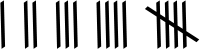
\includegraphics[width=0.3\textwidth]{turven}
\end{center}

%\newpage
\begin{stopdracht}
Stel nu een frequentietabel op voor jouw onderzoek. Je kan je laten leiden door bovenstaand
voorbeeld en de klassenbreedte gelijk aan 5 nemen, tenzij dat voor de data niet zinvol is.
\begin{center}
  \setlength{\tabcolsep}{5pt}
  \renewcommand{\arraystretch}{1}
  \begin{tabular}{|p{2cm}|p{2cm}|p{2cm}|p{2cm}|p{2cm}|p{2cm}|}
    \hline
    Klasse & Turf & Frequentie &&Relatieve Frequentie&\\
    \hline&&&&&\\\hline&&&&&\\\hline&&&&&\\\hline&&&&&\\\hline&&&&&\\
    \hline&&&&&\\\hline&&&&&\\\hline&&&&&\\\hline&&&&&\\\hline&&&&&\\
    \hline&&&&&\\\hline&&&&&\\\hline&&&&&\\\hline&&&&&\\\hline&&&&&\\\hline
  \end{tabular}
\end{center}
\end{stopdracht}

Naast de frequentie en de relatieve frequentie bestaan er ook nog de {\it cumulatieve} versies van deze frequenties. Cumulatief wil zeggen dat iets steeds toeneemt of ophoopt. In het geval van de frequentie is de {\bf cumulatieve frequentie} het aantal gegevens dat tot deze klasse en alle lagere klassen behoord. De {\bf relatieve cumulatieve frequentie} van een klasse is dan de verhouding van de cumulatieve frequentie van die klasse en het totale aantal gegevens.

\begin{stopdracht}
Vul de frequentietabel verder aan met de cumulatieve frequentie en de relatieve cumulatieve frequentie.
\end{stopdracht}

Als we enorm veel data hebben kan het berekenen van de klassen beter gebeuren door de computer. In Geogebra doen we dit als volgt:
\begin{enumerate}
  \item Plaats alle data in een lijst: vul hiervoor de eerste kolom van het rekenblad met de data, selecteer deze cellen en kies {\it creëer lijst} (rechts klikken). Noem de gemaakte lijst "data" door deze te hernoemen (lijst selecteren en "data" typen).
  \item Bereken het maximum en het minimum: voer de commando's \verb#min=Min[data]# en \verb#max=Max[data]# in.
  \item Bereken een goede klassenbreedte, bijvoorbeeld voor $10$ klassen vinden we $$\frac{max-min}{10}=\frac{81-42}{10}=3.9\;.$$ We ronden af en nemen als klassenbreedte $4$.
  \item Maak nu in het rekenblad een kolom voor linker- en rechter klassengrenzen. Dit gaat het snelst als je in \verb#C2# het getal $42$ plaatst. Nu is \verb#D2# gelijk aan de linker grens plus de klassenbreedte. Dus in \verb#D2# wordt 
  \begin{verbatim}
    =C2 + 4
  \end{verbatim} 
  geplaatst. \verb#C3# begint nu waar de vorig grens was geëindigd, plaats daar dus \verb#=D2#. Nu kunnen de correcte cellen naar beneden gesleept worden, Geogebra zal de correcte klassen creëren.
  \item Laat nu Geogebra zelf de gegevens turven, hiervoor vul je in \verb#E2# 
  \begin{verbatim}
    =TelAls[C2 <= x < D2, data]
  \end{verbatim}
  in. Er wordt in de data gekeken, en geteld hoeveel keer er een element tussen de klassengrenzen ligt.
\end{enumerate}

\begin{center}
  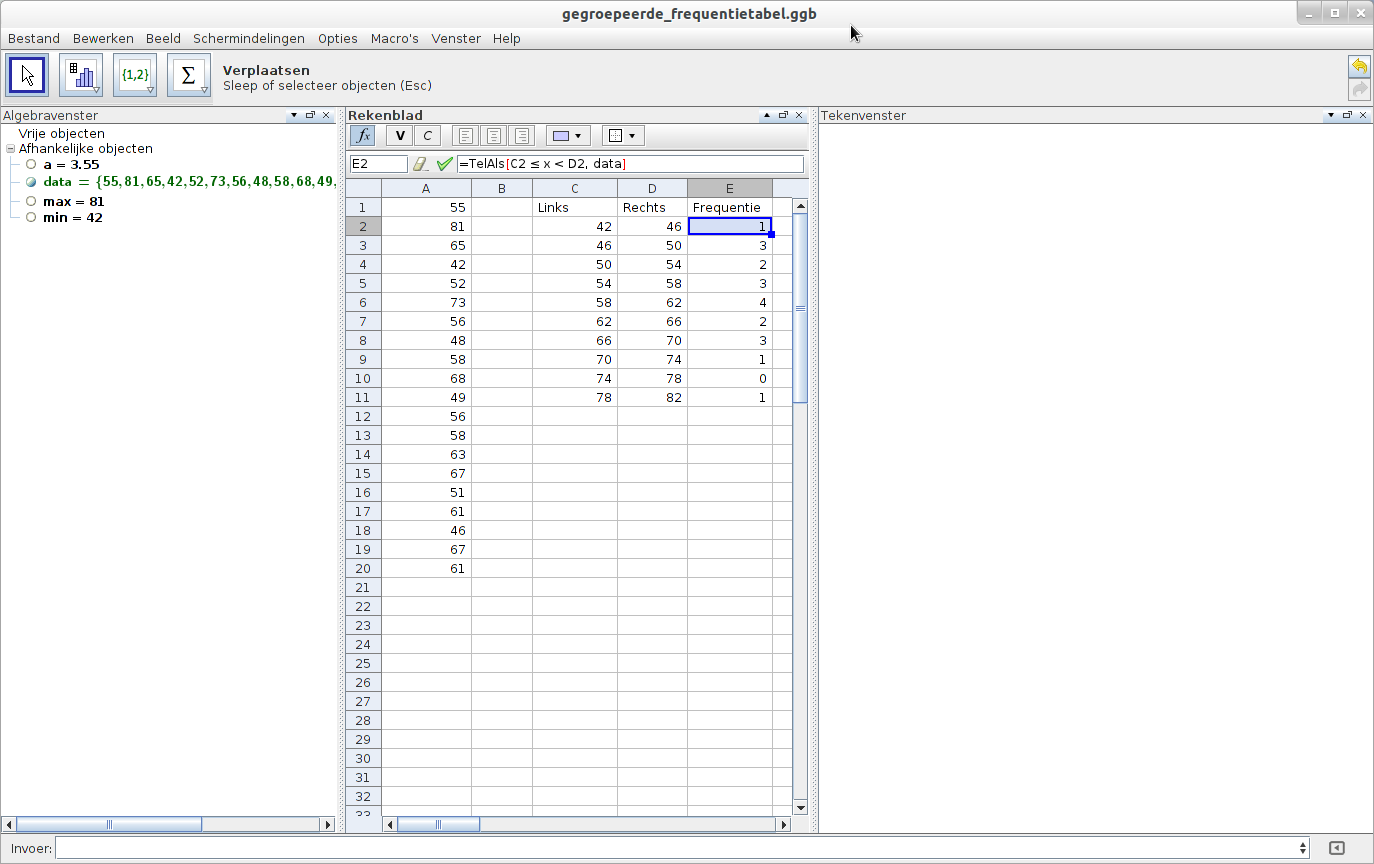
\includegraphics[width=14cm]{gg-gegroepeerde_frequentietabel}
\end{center}

\subsubsection{Het histogram}

Een {\bf histogram} is de meest gebruikte figuur om het globale gedrag van continu
kwantitatieve gegevens te onderzoeken. Deze stelt de frequentieverdeling bij klassenindeling
grafisch voor. We maken een histogram als volgt:

\begin{enumerate}
  \item Kies op de $x$-as een lengte-eenheid en breng op de $x$-as de beeldpunten van de klassengrenzen aan. Elke klasse komt dan overeen met een lijnstuk.
  \item De klassenfrequenties worden voorgesteld met behulp van rechthoeken die de horizontale lijnstukken op de $x$ as als zijde hebben. Dan moet de verticale zijde zo zijn, dat de oppervlakte van de bijbehorende rechthoek recht evenredig is met de frequentie van een klasse. We moeten dus de hoogte van elke rechthoek berekenen en vervolgens die rechthoeken construeren, allen aan de zelfde kant van de $x$-as.
\end{enumerate}

\begin{stopdracht}
Teken een histogram voor de opgestelde frequentietabel.
\begin{center}
\begin{tikzpicture}[line cap=round,line join=round,>=triangle 45,x=1.0cm,y=1.0cm]
\draw [gray, very thin, step=0.5cm] (0,0) grid (15,10);
\draw[-,black,very thick] (0,2) -- (15,2);
\draw[-,black,very thick] (2,0) -- (2,10);
\end{tikzpicture}
\end{center}
\end{stopdracht}

{\bf Verschil tussen een staafdiagram en een histogram:}\\
Sommigen denken dat een histogram en een staafdiagram goed op elkaar
lijken. Dat is fout, want er zijn fundamentele verschillen. Een histogram hoort
bij een continu kwantitatieve veranderlijke waar geen tussenstappen zijn tussen
de “mogelijke” uitkomsten. Bij een histogram liggen de rechthoeken dus tegen
elkaar. Bij een staafdiagram is er open ruimte tussen de staafjes. Bovendien
kijk je bij een staafdiagram naar de hoogte en bij een histogram naar de
oppervlakte.

Met Geogebra tekenen we als volgt het histogram:
\begin{enumerate}
  \item Gebruik de kolom met de linkergrenzen om een lijst te creëren. Noem deze lijst {\it grenzen} door ze te selecteren en te hernoemen. De laatste grens werd nog niet toegevoegd aan de lijst, om dit te doen kan je dubbelklikken op de lijst en er achteraan nog de juiste cel aan toevoegen.
  \item Selecteer nu de kolom met frequenties en creëer er de lijst {\it frequenties} mee.
  \item Voer nu het commando \verb#Histogram[grenzen,frequenties]# in. Geogebra maakt nu het histogram.
  \item Herschaal de assen, verplaats de $y$-as en vul de labels aan.
\end{enumerate}

\begin{center}
  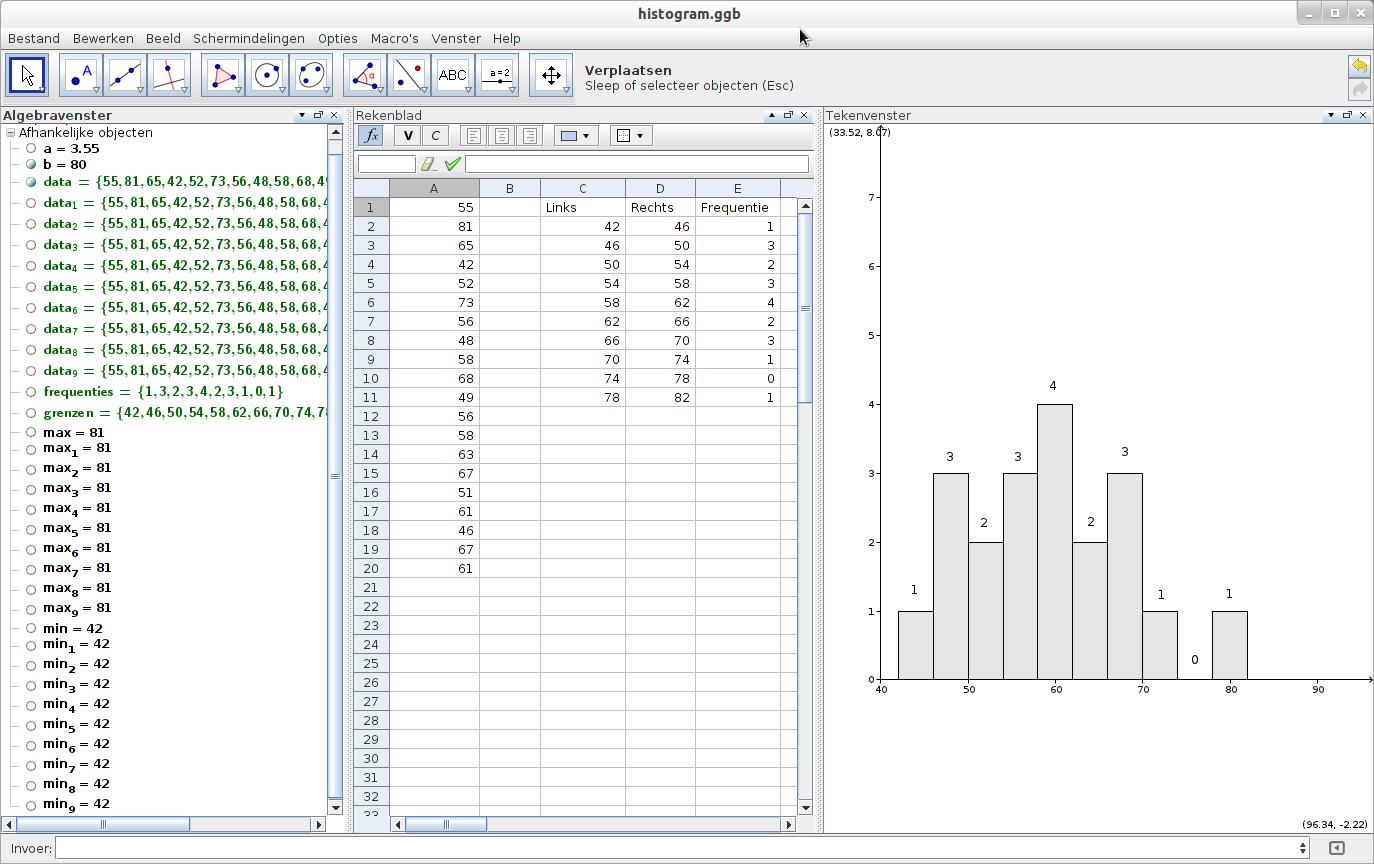
\includegraphics[width=14cm]{gg-histogram}
\end{center}

\subsubsection{Numerieke kenmerken: de kengetallen}

\subsubsection*{Gemiddelde en mediaan}

Hoe de testpersonen de tijdsduur van 1 minuut geschat hebben is mooi weergegeven
in het histogram. Maar wat doe je als men vraagt om al die informatie in enkele
getallen samen te vatten?

Een samenvatting in getallen (die {\bf kengetallen} worden genoemd) geeft je zelden evenveel
informatie als een goede figuur. Maar soms kan een kengetal dienen als “typisch” resultaat. Dat is
natuurlijk wel handig.

Als eerste kenmerk wil je weten hoelang een typische proefpersoon denkt dat een minuut duurt.
Daarom ga je op zoek naar een getal dat “het centrum” van al je resultaten weergeeft. Een
gebruikelijk kengetal hiervoor is het {\bf gemiddelde}. Een ander kengetal voor “centrum” is de
{\bf mediaan}.

Deze kengetallen kunnen enkel berekend worden bij kwantitatieve gegevens.

Bij {\bf discrete kwantitatieve gegevens} wordt het gemiddelde berekend door het quotiënt te nemen van hun som en hun aantal. De mediaan wordt berekend door de gegevens te rangschikken van klein naar groot en het middelste getal te nemen als het aantal gegevens oneven is of het gemiddelde te nemen van de middelste twee getallen als het aantal getallen even is.

Een simpel voorbeeld is:

\begin{oefening}
Bereken het gemiddelde van de volgende toetsresultaten: 4, 5.5, 6, 6, 6, 6.5, 7, 7, 7, 7.5, 7.5, 8, 8, 8, 8, 8.5, 8.5, 9, 9.5, 10, 10.\\
\ruitjes{3cm}
\end{oefening}

\begin{oefening}
Bereken de mediaan van de volgende toetsresultaten: 4, 5.5, 6, 6, 6, 6.5, 7, 7, 7, 7.5, 7.5, 8, 8, 8, 8, 8.5, 8.5, 9, 9.5, 10, 10.\\
\ruitjes{3cm}
\end{oefening}

In het vorige voorbeeld werd het gemiddelde en mediaan berekend van discrete kwantitatieve gegevens. Ons
onderzoek bevat {\bf continue kwantitatieve gegevens} die gegroepeerd zijn in een frequentietabel. Om hiervan
het gemiddelde te berekenen zoeken we van elke klasse het {\bf klassenmidden}, dit is de halve som van de
ondergrens en de bovengrens van die klasse. Bijvoorbeeld van de klasse $[42, 46[$ is het klassenmidden
$$
\frac{42 + 46}{2}=44\;.
$$

Dit klassenmidden wordt nu vermenigvuldigd met elke frequentie. Dit noemen we het product. Alle bekomen producten worden opgeteld. Het gemiddelde is dan het quotiënt van som van de producten en de som van de frequenties.
\newpage

\begin{stopdracht}
Bereken nu het gemiddelde.
\begin{center}
  \setlength{\tabcolsep}{7pt}
  \renewcommand{\arraystretch}{1.5}
  \begin{tabular}{|p{2cm}|p{3cm}|p{2cm}|p{2cm}|}
    \hline
    Klasse & Klassenmidden & Frequentie & Product\\
    \hline&&&\\\hline&&&\\\hline&&&\\\hline&&&\\\hline&&&\\
    \hline&&&\\\hline&&&\\\hline&&&\\\hline&&&\\\hline&&&\\
    \hline&&&\\\hline&&&\\\hline&&&\\\hline&&&\\\hline&&&\\\hline
    \multicolumn{2}{r|}{Som:} & &\\\cline{3-4}
  \end{tabular}
\end{center}
\vspace*{0.5cm}
Het gemiddelde is:
$$
\bar{x}=\frac{\phantom{.......................}}{\phantom{.....................}}=
$$
\vspace*{0.5cm}
\end{stopdracht}
\vspace*{-0.5cm}

Omdat onze gegevens gegroepeerd zijn moeten we bij het berekenden van de mediaan de gegevens ordenen van klein naar groot en kijken in welke klasse de middelste waarde zich bevind. Hiervoor hebben we dus de ruwe data nodig. Deze sorteren we van klein naar groot. De middelste waarde bij een oneven aantal gegevens bepaald de klasse waar de mediaan in ligt. Het klassenmidden is dan de mediaan. Bij een even aantal gegevens bepaald het gemiddelde van de twee middelste gegevens de klasse. De mediaan is dan ook het klassenmidden van deze klassen.

\newpage
\begin{stopdracht}
Bepaal de mediaan van ons onderzoek.\\
\ruitjes{4cm}
\end{stopdracht}

\subsubsection*{Standaardafwijking en interkwartielafstand}

Om je opmetingen te karakteriseren is het “centrum” maar een eerste stap. Een tweede karakteristiek
is de spreiding rond dit centrum. De gebruikelijke kengetallen hiervoor zijn de standaardafwijking en
de interkwartielafstand. Zij worden ook {\bf spreidingsmaten} genoemd.

Om de spreiding van de gegevens rond het gemiddelde te berekenen, gebruik je de
{\bf standaardafwijking} $s$. Voor de standaardafwijking bestaat een “te gekke” formule. Die ziet eruit als
$$
s = \sqrt{\frac{1}{n-1}\sum^n_{i=1}(x_i - \bar{x})^2}
$$
waarbij $n$ staat voor het aantal gegevens, $\bar{x}$ voor het gemiddelde en $x_i$ voor het $i$-de gegeven. Dit kengetal zullen we straks berekenen met software.

Een andere maat voor spreiding is de lengte van het gebied waarin de middelste 50\% van de
geordende opmetingen liggen. Dit gebied loopt van het {\bf eerste kwartiel} Q1 tot het {\bf derde kwartiel} Q3.
De lengte van dit interval is de {\bf interkwartielafstand}, genoteerd als IQR (= InterQuartile Range).
Als we de reeds berekende mediaan Q2 noemen, dan is Q1 te bepalen door de mediaan te nemen van de
gegevens links van Q2 en Q3 is te bepalen door de mediaan te nemen van de gevens rechts van Q2. Ook
dit kengetal zullen we berekenen met software.

\subsubsection{Berekenen van de 1-variabele statistieken}

Alle voorgaande kengetallen vatten we samen met de {\bf 1-variabele statistieken}. Deze kunnen allemaal
in één keer berekend worden met Geogebra. Selecteer hiervoor de lijst met data en kies het icoon 
{\it onderzoek één variabele}. Verschuif het aantal klassen naar $10$. Geogebra zal het histogram plotten
een lijst geven met kengetallen.

De volgende zijn belangrijk:
\begin{center}
  \begin{tabular}{r|l}
    $n$ & Het aantal gegevens.\\
    Gemiddelde & Het rekenkundig gemiddelde.\\
    $s$ & De standaard afwijking.\\
    Min & De laagste waarde.\\
    Q1 & Het eerste kwartiel.\\
    Mediaan & De mediaan.\\
    Q3 & Het derde kwartiel.\\
    Max & De hoogste waarde.\\
  \end{tabular}
\end{center}

\begin{center}
  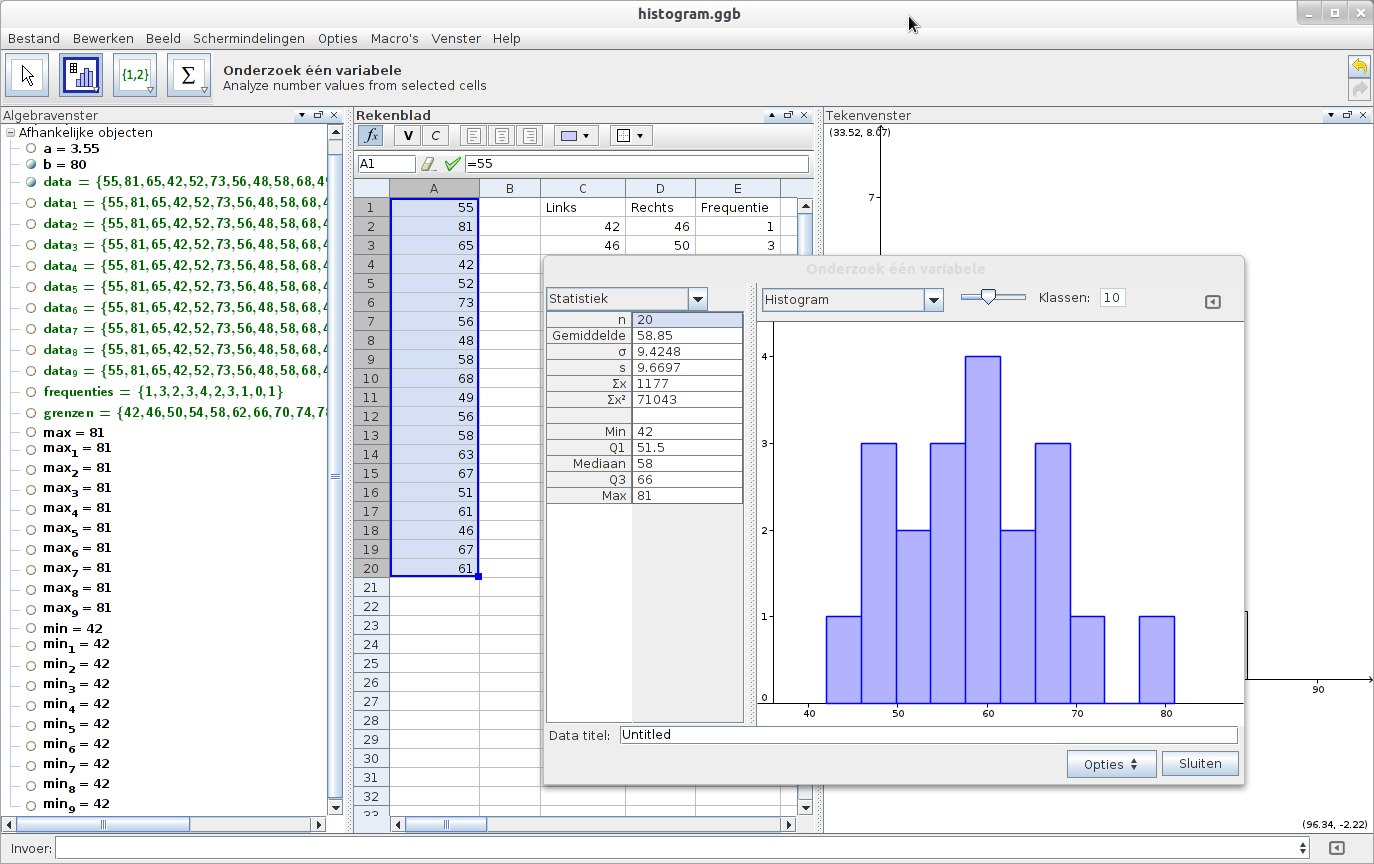
\includegraphics[width=14cm]{gg-1var_stat}
\end{center}

\subsubsection{De boxplot}

\begin{wrapfigure}[10]{l}{0.4\textwidth}
  \vspace{-1cm}
  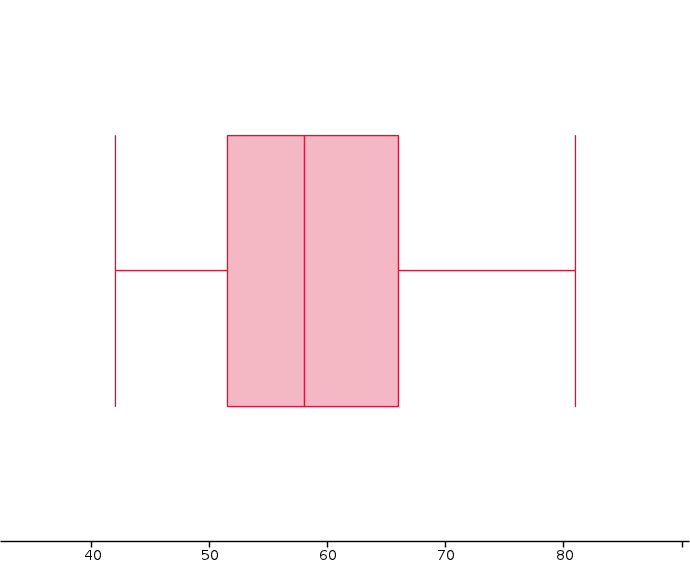
\includegraphics[width=0.4\textwidth]{boxplot}
\end{wrapfigure}

Een goed zicht op zowel het centrum als de spreiding van je opmetingen, krijg je uit een boxplot. Dit
is een grafiek die gebruik maakt van de begrippen minimum, maximum, mediaan, eerste kwartiel
Q1, derde kwartiel Q3, IQR en uitschieters.

De rechterstaart begint vanaf Q3. Dit lijnstuk gaat tot aan de grootste opmeting die kleiner of
gelijk is aan $\mbox{Q3} + (1.5\cdot\mbox{IQR})$. Elke observatie die nog groter is, wordt als een uitschieter
beschouwd en apart aangeduid. In deze studie loopt de rechterstaart van $66$ tot $81$ en heeft
dus een lengte van $15$. Op een analoge manier teken je de linkerstaart, links van Q1. Die
loopt hier van $42$ tot $51.5$, wat een lengte van $9.5$ oplevert.
De rechthoekjes duiden aan waar de middelste getallen van de dataset liggen. De
linkerrechthoek gaat van Q1 tot Med. In dat gebied ligt het tweede kwart van de geordende
getallen. De rechterrechthoek gaat van Med tot Q3, en daar ligt het derde kwart van deze
getallen.

\begin{stopdracht}
Teken nu de boxplot van het onderzoek. Vergeet de x-as niet te voorzien van de juiste getallen en de juiste eenheid.
\ruitjes{6cm}
\end{stopdracht}

\begin{stopdracht}
Zijn er uitschieters in je dataset? Was dat te verwachten?
\arules{3}
\end{stopdracht}

In Geogebra krijg je een boxplot door in het venster van de 1-variabele statistieken {\it Boxplot} te kiezen in plaats van {\it Histogram}.

\begin{center}
  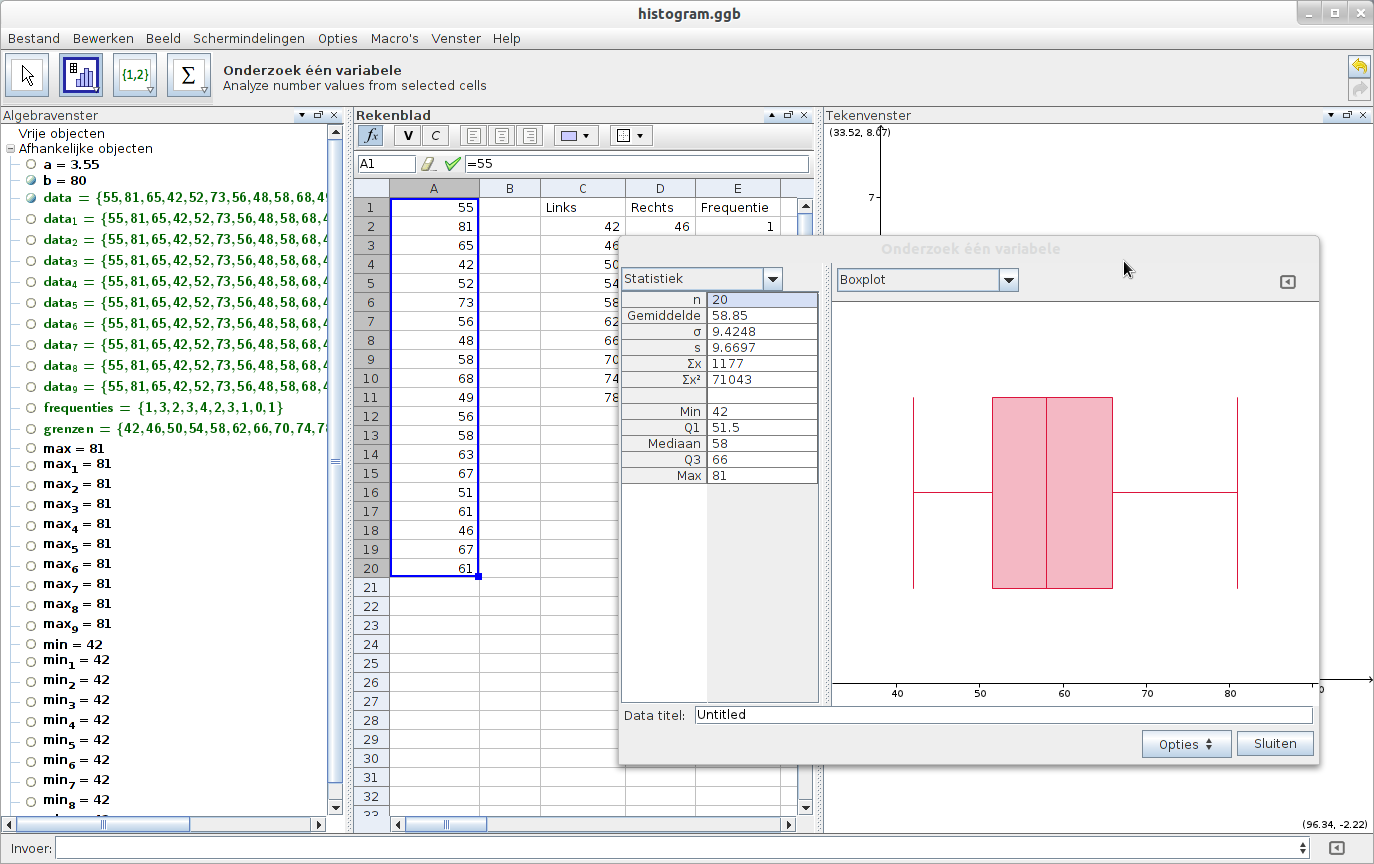
\includegraphics[width=14cm]{gg-boxplot}  
\end{center}

\subsection{Wat heb je gevonden? Hoever kan je gaan in je conclusie?}

\subsubsection{De variabiliteit van steekproefresultaten}

Je bent er nu al mee vertrouwd. Een steekproef levert toevallige resultaten op, en bij een andere
steekproef krijg je andere resultaten. Indien je de populatie van alle leerlingen van je school in
identieke omstandigheden de tijdsduur van één minuut zou laten schatten, dan zou het gemiddelde
van al die schattingen niet exact samenvallen met het gemiddelde dat jij in je steekproef hebt
gevonden. Dat is niet erg. De statistiek is er juist om je te helpen om goede uitspraken over de
populatie te doen. Als er tenminste geen andere problemen opduiken... .

In dit onderzoek heb je elke leerling aan een kleine test onderworpen. De manier waarop die test
moet worden afgenomen heb je vooraf heel precies vastgelegd, en je hebt je aan die procedure strikt
gehouden bij elke leerling die je hebt getest. Maar er is nog iets anders dat voor fouten kan zorgen.
Je werkt met meetapparatuur, en is die wel goed geijkt? Als je een chronometer gebruikt die start bij
2 in plaats van bij 0, dan heb je in al je opmetingen een systematische fout van 2 seconden. Je krijgt
dan een vertekend beeld van de werkelijkheid.

Als al je opmetingen op een systematische manier te klein (of te groot) zijn dan heb je {\bf vertekening}.
Vertekening in metingen kan je met statistiek niet opsporen. Je moet vooraf controleren of je
apparatuur wel juist geijkt is. Doe dit vooraleer je aan je onderzoek begint!

\begin{oefening}
Je moet de lengte van 20 planken meten en je doet dat met een rolmeter. Op welke manier
zou hier vertekening kunnen optreden?
\arules{3}
\end{oefening}

\begin{center}
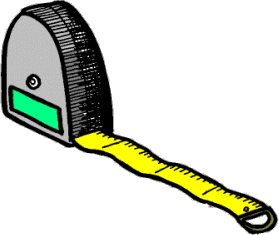
\includegraphics[width=5cm]{rolmeter}
\end{center}

\begin{oefening}
Soms kan je op een spitsvondige manier vertekening in opmetingen neutraliseren. Als je een
weegschaal moet gebruiken waarvan je vermoedt dat zij systematisch een te laag gewicht
aangeeft, hoe zou jij dan een boekentas daarop wegen, als je met die weegschaal vooraf niets
mag doen?
\ruitjes{7cm}
\end{oefening}

\subsubsection{Een uitspraak over de populatie}

Wat we in het “exploratief” onderzoek hebben gevonden is van toepassing op de dataset die we hebben
onderzocht, en dus op alle leerlingen van de klas. Als je op een goede manier een steekproef trekt, als je je
strikt houdt aan de procedure om de leerlingen te testen, en als je meetapparatuur goed geijkt is, dan
kan je met statistiek verantwoorde uitspraken doen over hoe heel de school een minuut zou schatten.
Voor deze steekproef was het gemiddelde $58.85$ seconden en de mediaan was $58$ seconden. Dat ligt
niet ver uit elkaar, en je zou kunnen vermoeden dat het gemiddelde en de mediaan van de hele
populatie ook wel in de buurt van $58$ seconden liggen. Waarschijnlijk is dat nog waar ook.

\subsection{Kernachtige samenvatting van dit onderzoek}

Je samenvatting bestaat uit twee delen
\begin{enumerate}
  \item De antwoorden op de contextvragen (de www-vragen),
  \item De besluiten over het uitgevoerde onderzoek.
\end{enumerate}

Betrek ook de kengetallen in je besluit: vermeld hun getalwaarde en ga na in hoever ze een zinvolle
karakteristiek zijn voor dit onderzoek. Vergeet ook nooit om goede grafieken te tekenen en die te
interpreteren.

\begin{stopdracht}
Formuleer nu de antwoorden op de contextvragen (de www-vragen).
\arules{8}
\end{stopdracht}

\begin{stopdracht}
Formuleer nu de besluiten over het uitgevoerde onderzoek.
\arules{8}
\end{stopdracht}

\newpage
\subsection{Zelfevaluatie}

In dit onderzoek heb je geleerd over:
\begin{itemize}
  \item vertekening bij opmetingen
  \item de continu kwantitatieve veranderlijke
  \item de frequentietabel met klassenindeling
  \item het histogram en de boxplot
  \item het gemiddelde en de mediaan
  \item de standaardafwijking en de interkwartielafstand
  \item de interpretatie van kengetallen in combinatie met grafieken
\end{itemize}

Je bent nu in staat om volgende opdrachten uit te voeren:

\begin{oefening}
Wanneer is een kwantitatieve veranderlijke continu? Zeg dat in je eigen woorden, en geef
enkele voorbeelden.
\arules{6}
\end{oefening}

\begin{oefening}
Schrijf je een continu kwantitatieve veranderlijke altijd op met kommagetallen? Motiveer je
antwoord.
\arules{6}
\end{oefening}

\begin{oefening}
Welke eigenschap probeert de standaardafwijking te beschrijven? Zeg in woorden hoe je de
standaardafwijking berekent. Kan je daaruit afleiden of de standaardafwijking gevoelig is
voor uitschieters? Kan je daarvan een eenvoudig voorbeeld geven?
\arules{6}
\end{oefening}

\begin{oefening}
Welke eigenschap probeert de interkwartielafstand te beschrijven? Zeg in woorden wat
kwartielen zijn en hoe je de interkwartielafstand berekent. Kan je daaruit afleiden of de
interkwartielafstand gevoelig is voor uitschieters? Kan je daarvan een eenvoudig voorbeeld
geven?
\arules{6}
\end{oefening}

\newpage
\section*{Voorbeeld examen}
\vraag{14}
Van de {\em sweet \& fair shop} krijg je de volgende dataset\footnote{Met dank aan de studenten van 6SETA.}:

druivensuiker aardbei; druivensuiker mango; kinderrozijnen; amandel chocolades; zure frieten; zure frieten; coco-mango reep; koban mix; kinderrozijnen; druivensuiker mango; zure frieten; kinderrozijnen;  druivensuiker mango; druivensuiker aardbei;  druivensuiker mango; druivensuiker mango; druivensuiker mango; druivensuiker aardbei; druivensuiker aardbei; druivensuiker aardbei; druivensuiker aardbei; kinderrozijnen;

Stel een frequentietabel op:
\begin{center}
  \begin{tabular}{p{4cm}|p{4cm}|p{4cm}}
    &absolute frequentie&relatieve frequentie\\
    \hline
    &&\\[6cm]
  \end{tabular}
\end{center}

Wat heb je genomen als veranderlijke? \arulefill
Dit is een kwalitatieve/kwantitatieve veranderlijke. {\tiny (schrappen wat niet past)}
Wat is de steekproefgrootte? \arulefill
Er zijn twee manieren om de data grafisch voor te stellen, welke:
\begin{itemize}
  \item \arule{6cm}
  \item \arule{6cm}
\end{itemize}

\newpage
Stel je data grafisch voor (op twee manieren)

\ruitjes{20cm}

\newpage
\vraag{16}
Aan een aantal studenten uit het eerste jaar hoger onderwijs werd gevraagd hoeveel auto's er bij hen in het gezin waren. De data die we terugkregen was als volgt:
2; 0; 3; 1; 1; 1; 3; 1; 1; 1; 2; 1; 0; 0; 2; 0; 0; 0; 7; 1; 2; 2; 2; 2; 1; 1; 1; 2; 2; 3

Wat zijn de elementen in dit onderzoek?
\arules{1}

Welke veranderlijke wordt hier onderzocht?
\arules{1}

Waarom mag je zeggen dat de veranderlijke in dit onderzoek kwantitatief is?
\arules{2}

Is de kwantitatieve veranderlijke discreet of continue?
\arules{1}

Vervolledig de frequentietabel (het is niet nodig om de data in klassen op te delen):
\begin{center}
  \setlength{\tabcolsep}{7pt}
  \renewcommand{\arraystretch}{1.5}
  \begin{tabular}{p{4cm}|p{4cm}|p{4cm}}
    &&\\
    \hline
    0&&\\
    1&&\\
    2&&\\
    3&&\\
    4&&\\
    5&&\\
    6&&\\
    7&&\\
    &n=&\\
  \end{tabular}
\end{center}

Maak een histogram waarin je absolute frequenties gebruikt.

\begin{center}
\definecolor{cqcqcq}{rgb}{0.65,0.65,0.65}
\begin{tikzpicture}[xscale=1,yscale=0.3,line cap=round,line join=round,>=triangle 45,x=1.0cm,y=1.0cm]
\draw [color=cqcqcq,dash pattern=on 1pt off 1pt, xstep=1.0cm,ystep=1.0cm] (-1,-1) grid (12,12);
\draw[->,color=black] (-1,0) -- (12,0);
\draw[shift={(1,0)},color=black] (0pt,2pt) -- (0pt,-2pt) node[below] {\footnotesize $1$};
\draw[color=black] (0.25,12.07) node [anchor=south west] { x};
\draw[->,color=black] (0,-1) -- (0,12);
\draw[shift={(0,1)},color=black] (2pt,0pt) -- (-2pt,0pt) node[left] {\footnotesize $1$};
\draw[color=black] (12.09,-1.25) node [anchor=west] { y};
\draw[color=black] (0pt,-10pt) node[right] {\footnotesize $0$};
\end{tikzpicture}
\end{center}

Is het belangrijk de grootste absolute frequentie vooraan wordt geplaatst?
\arules{1}

In hoeveel gezinnen zijn er $4$ auto's? \arulefill
Waarom staat de waarde $4$ dan toch in de frequentietabel?
\arules{3}

Is het nuttig om ook in het histogram een plaatsje op de $x$-as te voorzien voor $4$ auto's, hoewel er daar geen staaf getekend is?
\arules{2}

Bereken het gemiddeld aantal auto's per gezin:
%\vspace*{1cm}
$$\bar{x}=\arule{5cm}$$

Voor wat is het gemiddelde gevoelig?
\arules{1}

Wat is de oplossing hierop?
\arules{1}

Geef deze voor ons voorbeeld:
\arules{1}

\newpage
\vraag{10}
Tijdens de opendeurdag laat de afdeling hout de leerlingen uit het zesde leerjaar planken zagen op 180 cm. Na tien planken meten we de reeds gezaagde planken en we vinden de volgende lengtes:\\
177; 178; 178; 179; 179; 180; 181; 181; 183; 184 cm\\

{\em Bereken of bepaal en geef ook steeds het correcte symbool!}

Steekproefgrootte:\arulefill

Gemiddelde:\arulefill

Standaard afwijking\footnote{$s = \sqrt{\frac{\mbox{som van alle gekwadrateerde afwijkingen t.o.v. het gemiddelde}}{n-1}} = \sqrt{\frac{\sum_{i=0}^n(\bar{x}-x_i)^2}{n-1}}$}:\arulefill

Maximum:\arulefill

Minimum:\arulefill

Eerste kwartiel:\arulefill

Mediaan:\arulefill

Derde kwartiel:\arulefill

Interkwartielafstand:\arulefill

Teken de boxplot:

\ruitjes{3cm}

\end{document}

\newpage
\section{Projecten}

Kies één van volgende projecten om zelf een onderzoek rond uit te voeren:

\vraag{Je wenst als dierenarts te beginnen in een stad. Om te kunnen inschatten hoeveel
'klanten' je zal hebben wil je weten hoeveel huisdieren er ongeveer zijn in het dorp. Je
kan uiteraard niet bij iedereen langs gaan. Zet een onderzoek op om het totaal aantal
huisdieren in te schatten.}{1cm}


\vraag{Een fietsenmaker wenst voor de nieuwe collectie 20 MTB te kopen. Hij weet alleen
niet goed welke kleuren hij zou nemen. Hij weet dat jij reeds statistiek hebt gevolgd en vraagt
je raad. Hoe zul je dit aanpakken. Wat is de populatie, wat is een goede steekproef? Zal de
data bestaan uit kwantitatieve of kwalitatieve gegevens?}{1cm}

\vraag{De leesbaarheid van een tekst hangt onder meer af van de lengte van de zinnen. Korte zinnen
lezen gemakkelijker dan lange zinnen. Als je aanneemt dat zowat elke nieuwe zin met een
hoofdletter begint, en dat er verder niet te veel afkortingen in hoofdletters voorkomen, dan is
de verhouding van het aantal hoofdletters ten opzichte van het totale aantal letters een goede
maat voor de lengte van de zinnen. Het is nu aan jou om voor deze werktekst een goede schatting te
maken van de proportie hoofdletters. Hoe ga je dat doen? Is er een mogelijkheid om een getrapte
steekproef te nemen?}{1cm}

\vraag{Stel zelf een onderzoek op naar iets dat je interesseert. Bepaal eerst een goede
onderzoeksvraag. Bepaal daarna pas de populatie en geef dan een methode om een steekproef
te nemen.}{1cm}

Kijk steeds eerst wat je wilt weten en hoe je gaat meten. Onderzoek dan de dataset en trek je
conclusies. Geef op het einde een samenvatting van het onderzoek.

\end{document}

\begin{thebibliography}{1}
\bibitem{1}\label{1} Prof. dr. Herman Callaert, Hans Bekaert, Celine Goethals, Lies Provoost, Marc Vancaudenberg, \textit{Exploratieve statistiek, Werktekst voor de leerling}, Centrum voor statistiek, Universiteit Hasselt, 2005\\
\bibitem{2}\label{2} J.-P. Daems, E. Jennekens, \textit{Argument, Algebra - Meetkunde - Driehoeksmeting}, Uitgeverij de boeck, 2003\\
\end{thebibliography}

%Deze bundel is grotendeels gebaseerd op \cite{1}. Hiervoor werd toestemming verleend. Voor correcties, meer informatie of een nieuwere versie kan ik gecontacteerd worden op \href{mailto:pieter.pareit@ugent.be}{pieter.pareit@ugent.be}.


\end{document}


\begin{wrapfigure}[13]{r}{0.3\textwidth}
  \includegraphics[width=0.3\textwidth]{figuur}
\end{wrapfigure}

\begin{center}
  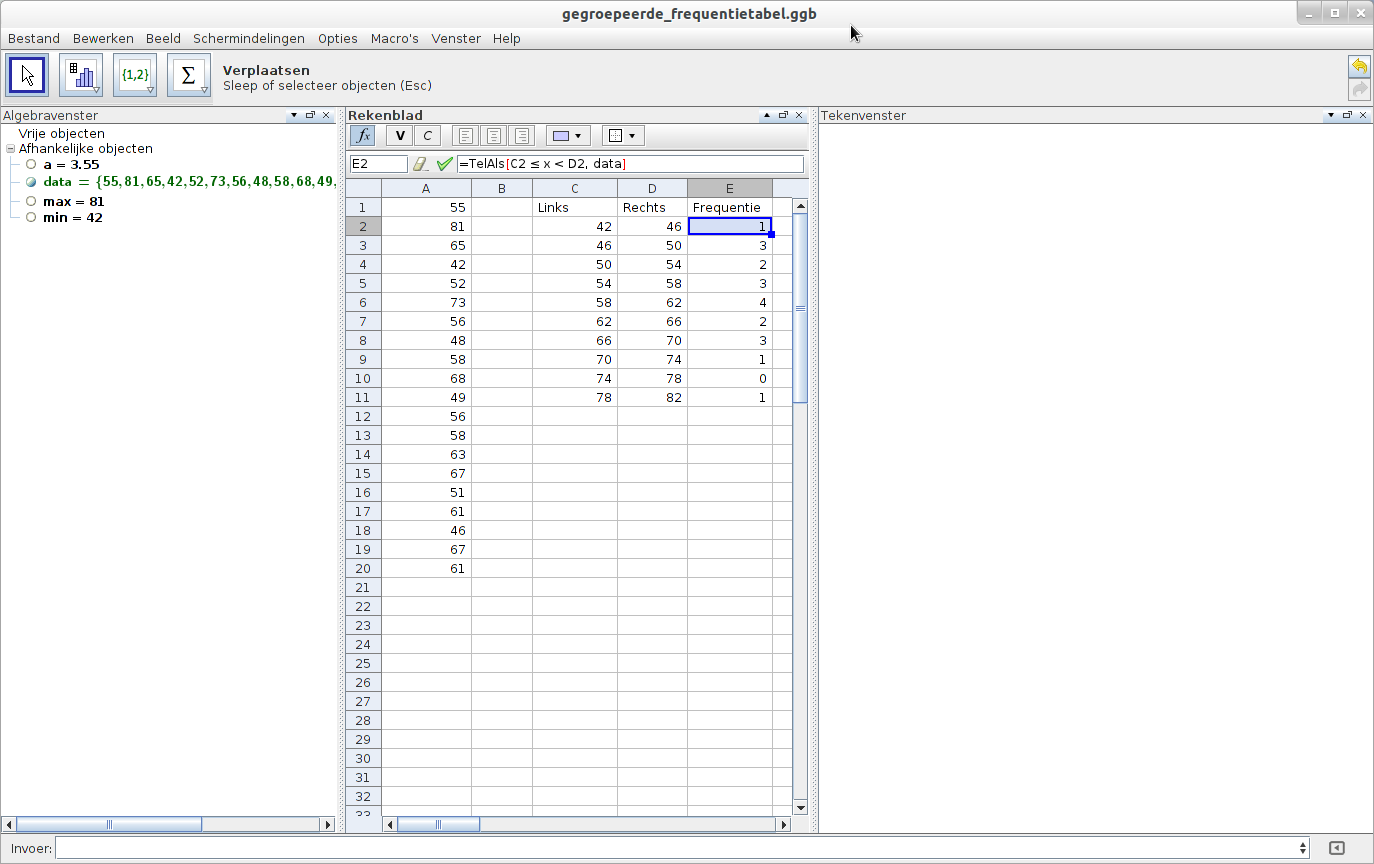
\includegraphics[width=14cm]{gg-gegroepeerde_frequentietabel}
\end{center}































